\documentclass[11pt]{book}
\usepackage{geometry}                % See geometry.pdf to learn the layout options. There are lots.
\usepackage{graphicx}
\usepackage{epstopdf}
\usepackage{amssymb,amsmath}
\usepackage[charter]{mathdesign}
\usepackage{multirow}
\DeclareGraphicsRule{.tif}{png}{.png}{`convert #1 `dirname #1`/`basename #1 .tif`.png}

\usepackage[colorlinks=true,linkcolor=blue]{hyperref}

\textwidth6.5in
\textheight9.0in
\topmargin-0.5in
\oddsidemargin0in
\evensidemargin0in

\title{Material Models Used in NairnMPM and NairnFEA}
\author{John Nairn}
\date{\today} 

\font\tenbsf=cmssbx10 at 11pt
\font\bfsym=cmmib10 at 11pt

\renewcommand{\vec}[1]{\boldsymbol{#1}}
\newcommand{\tens}[1]{\boldsymbol{\mathsf{#1}}}

% definitions
%\def\C{{\fam=9 C}}
\def\A{\hbox{\tenbsf A}}
\def\a#1{\alpha_{#1}}  
\def\B{\hbox{\tenbsf B}}
\def\b#1{\beta_{#1}}  
\def\C{\hbox{\tenbsf C}}
\def\D{\hbox{\tenbsf D}}
\def\E{\hbox{\tenbsf E}}
\def\dev{\hbox{\tenbsf s}}
\def\ndev{\hbox{\tenbsf n}}
\def\cex{\vec{c}_{excess}}
\def\code#1{{\small\tt #1}}
\def\del{d \vec{\varepsilon}_{e}}
\def\dpl{d \vec{\varepsilon}_{p}}
\def\deff{d \vec{\varepsilon}_{tot}}
\def\df{d \vec{f}}
\def\dfa{d \vec{f}^\alpha}
\def\dfq{d \vec{f}^q}
\def\da{d\vec{\alpha}}
\def\dfW{{\partial f\over \partial W_p}}
\def\dsig{d \vec{\sigma}}
\def\DT{\Delta T}
\def\dq{d\vec q}
\def\dWp{dW_p}
\def\e#1{\varepsilon_{#1}}
\def\ee{\varepsilon}
\def\er#1{\varepsilon_{#1}^{(res)}}
\def\err#1{\varepsilon_{#1}^{(res,r)}}
\def\f{\hbox{\tenbsf f}}
\def\F{\hbox{\tenbsf F}}
\def\dF{\hbox{\tenbsf dF}}
\def\fvvec#1#2#3#4#5#6{\left(\begin{array}{ccc} #1 \\ #2 \\ #3 \\ #4 \\ #5 \\ #6 \end{array}\right)}
\def\g#1{\gamma_{#1}}  
\def\I{\hbox{\tenbsf I}}
\def\P{\hbox{\tenbsf P}}
\def\Q{\hbox{\tenbsf Q}}
\def\R{\hbox{\tenbsf R}}
\def\dR{\hbox{\tenbsf dR}}
\def\S{\hbox{\tenbsf S}}
\def\s#1{\sigma_{#1}}  
\def\symmat#1#2#3#4#5#6{\left(\begin{array}{ccc} #1 & #2 & #3 \\ #2 & #4 & #5 \\
                                                      #3 & #5 & #6 \end{array}\right)}
\def\t#1{\tau_{#1}}  
\def\v#1{\nu_{#1}}  
\def\vvec#1#2#3{\left(\begin{array}{ccc} #1 \\ #2 \\ #3 \end{array}\right)}
\def\w#1{\omega_{#1}} 

\def\Jeff{J_{eff}}
\def\Jres{J_{res}} 
\def\V{\hbox{\tenbsf V}}
\def\dV{\hbox{\tenbsf dV}}
\def\U{\hbox{\tenbsf U}}
\def\dU{\hbox{\tenbsf dU}}

\font\bfsym=cmmib10 at 10pt
\def\st{{\hbox{\bfsym\char'033}}}
\def\et{{\hbox{\bfsym\char'042}}}
\def\wt{{\hbox{\bfsym\char'041}}} 

\begin{document}
\maketitle

\tableofcontents

\chapter{Linear Elastic Hypoelastic Materials}

\section{Introduction}

The \code{Isotropic}, \code{TransIsotropic}, and \code{Orthotropic} classes all inherit from the \code{Elastic} class and implement linear elastic materials. The constitutive law is in the \code{Elastic} class and implemented for an orthotropic material. The isotropic and transversely isotropic materials are special cases of the orthotropic material. In MPM, isotropic materials have a separate constitutive law to enhance efficiency by ignoring terms that only apply to anisotropic materials. For such a material, the 3D stiffness equation in the material axis system is
\begin{equation}
     \left(\begin{array}{c} \s{xx} \\ \s{yy} \\ \s{zz} \\ \t{xz} \\ \t{yz} \\ \t{xy} \end{array}\right)
       =  \left(\begin{array}{cccccc}
      C_{11} & C_{12} & C_{13} & 0 & 0 & 0 \\
      C_{12} & C_{22} & C_{23} & 0 & 0 & 0 \\
      C_{13} & C_{23} & C_{33} & 0 & 0 & 0 \\
      0 & 0 & 0 & C_{44} & 0 & 0 \\
      0 & 0 & 0 & 0 & C_{55} & 0  \\
      0 & 0 & 0 & 0 & 0 &  C_{66}  \end{array}\right)
     \left(\begin{array}{c} \e{xx} -\er{xx} \\ \e{yy} -\er{yy} \\ \e{zz} -\er{zz}\\ 
                   \g{xz} \\ \g{yz} \\ \g{xy} \end{array}\right)
\end{equation}
The elements of the $\C$ matrix can be found from all engineering properties. Where $\er{ii}$ are  residual strains in the normal directions. Here they may be caused by either thermal expansion or moisture expansion:
\begin{equation}
\left(\begin{array}{c} \er{xx} \\ \er{yy} \\ \er{zz} \end{array}\right)
       =  \left(\begin{array}{c}
	\a{xx}\DT + \b{xx}\Delta c \\
	\a{yy}\DT + \b{yy}\Delta c \\
	\a{zz}\DT + \b{zz}\Delta c  \end{array}\right)
\end{equation}
where $\a{ii}$ and $\b{ii}$ are thermal and moisture expansion coefficients, and $\DT$ and $\Delta c$ are temperature and moisture change from reference conditions. FEA has only thermal expansion while MPM may have both thermal and moisture expansion.

\section{Plane Stress Equations}

The plane stress stiffness equations for in-plane stresses are
\begin{equation}
      \vvec{\s{xx}}{\s{yy}}{\t{xy}} = \symmat{Q_{xx}}{Q_{xy}}{0}{Q_{yy}}{0}{Q_{xyxy}}
          \vvec{\e{xx} - \er{xx}}{\e{yy} - \er{yy}}{\g{xy}}
 \end{equation}
The elements of the $\Q$ matrix are found from
\begin{eqnarray}%
   Q_{xx} &  = &  {E_{xx}\over 1 - \v{xy}\v{yx}} \\
   Q_{yy} & = & {E_{yy}\over 1 - \v{xy}\v{yx}} \\
   Q_{xy} &  = & {E_{xx}\v{yx}\over 1 - \v{xy}\v{yx}}  =  {E_{yy}\v{xy}\over 1 - \v{xy}\v{yx}}\\
   Q_{xyxy} & = &  G_{xy} 
\end{eqnarray}%
These elements are calculated in \code{SetAnalysisProps()} as \code{C11} = $Q_{xx}$, \code{C12} = $Q_{xy}$, \code{C22} = $Q_{yy}$, and \code{C66} = $Q_{xyxy}$. The thermal  and moisture expansion coefficients are equal to the material thermal  and moisture expansion coefficients and set as \code{CTE1} $=\a{xx}$, \code{CTE2} $=\a{yy}$, \code{CME1} $=\b{xx}$, and \code{CME2} $=\b{yy}$, also in \code{SetAnalysisProps()}.

In plane stress analysis, $\s{zz}=0$, but $\e{zz}\ne0$. The out-of-plane strain is found from the 3D stiffness matrix by solving the $\s{zz}$ equation for $\e{zz}$:
\begin{equation}
            \e{zz} = -{C_{13}\over C_{33}}(\e{xx} -\er{xx}) - {C_{23}\over C_{33}}(\e{yy} -\er{yy}) 
                     + \er{zz}
\end{equation}
The new terms are set in \code{SetAnalysisProps()} as \code{C13} $=-C_{13}/C_{33}$, \code{C23} $=-C_{23}/C_{33}$, \code{CTE3} $=\a{zz}$, and \code{CME3} $=\b{zz}$.

\section{Plane Strain Equations}

The plane strain stiffness equations for in-plane stresses are
\begin{equation}
      \vvec{\s{xx}}{\s{yy}}{\t{xy}} = \symmat{C_{11}}{C_{12}}{0}{C_{22}}{0}{C_{66}}
          \vvec{\e{xx} -\err{xx}}{\e{yy} - \err{yy}}{\g{xy}}
 \end{equation}
 where residual strains now depend on reduced residual strains
\begin{equation}
\left(\begin{array}{c} \err{xx} \\ \err{yy}  \end{array}\right)
       =  \left(\begin{array}{c}
	 \er{xx} + \v{zx}\er{zz} \\
	\er{yy} + \v{zy}\er{zz} \end{array}\right)
\end{equation}
which is equivalent to using reduced expansion properties
\begin{equation}
\left(\begin{array}{c} \err{xx} \\ \err{yy}  \end{array}\right)
       =  \left(\begin{array}{c}
	 \a{xx}^{(r)}\DT + \b{xx}^{(r)}\Delta c \\
	\a{yy}^{(r)}\DT + \b{xx}^{(r)}\Delta c \end{array}\right)
\end{equation}
The reduced expansion coefficients are
\begin{eqnarray}%
   \a{xx}^{(r)} = \a{xx} + \v{zx}\a{zz}, \ \ 
   \a{yy}^{(r)} = \a{yy} + \v{zy}\a{zz}, \ \ 
   \b{xx}^{(r)} = \b{xx} + \v{zx}\b{zz}, \ \ 
   \b{yy}^{(r)} = \b{yy} + \v{zy}\b{zz}
\end{eqnarray}%
These elements are calculated in \code{SetAnalysisProps()} as \code{C11} $=C_{11}$, \code{C12}  $=C_{12}$, \code{C22} $=C_{22}$, and \code{C66} $=C_{66}$. The reduced expansion coefficients are set as \code{CTE1} $=\a{xx}^{(r)}$, \code{CTE2} $=\a{yy}^{(r)}$, \code{CME1} $=\b{xx}^{(r)}$, and \code{CME2} $=\b{yy}^{(r)}$, also in \code{SetAnalysisProps()}.

In plane strain analysis, $\e{zz}=0$, but $\s{zz}\ne0$. The out-of-plane stress is found from the 3D stiffness matrix by setting $\e{zz}=0$:
\begin{eqnarray}
            \s{zz} & = & C_{13}\bigl(\e{xx} -(\a{xx}^{(r)}-\v{zx}\a{zz})\DT - (\b{xx}^{(r)}-\v{zx}\b{zz})\Delta c\bigr)
 \nonumber\\
 &&\qquad\mbox{}
                     +C_{23}\bigl(\e{yy} -(\a{yy}^{(r)}-\v{zy}\a{zz})\DT-(\b{yy}^{(r)}-\v{zy}\b{zz})\Delta c\bigr) 
                     -C_{33} \er{zz}
\end{eqnarray}
The new terms are set in \code{SetAnalysisProps()} as \code{C13} $=C_{13}$, \code{C23} $=C_{23}$, and \code{C33} $=C_{33}$. Notice that this equation needs actual residual expansion coefficients and thus the reduced expansion coefficients must be {\em unreduced} by subtracting terms. For these calculations (more details in next section), the following expansion properties are set as \code{CTE3} $=\a{zz}$, \code{CME3} $=\b{zz}$, \code{prop1} $=\v{zx}$, and \code{prop2} $=\v{zy}$.

\section{Rotated Stiffness Equations in 2D MPM}

For orthotropic materials with material angle not zero, the stiffness equations must be rotated counter-clockwise by the material point angle to transpose to the analysis coordinate systems. The initial material point angle is stored for anisotropic materials. To account for large rotations, the total angle from material axes to current axes must be found by polar decomposition of $\F$ (which can find $\sin\theta$ and $\cos\theta$ easily in 2D). Thus prior to calling \code{MPMConstitutiveLaw()}, the equations are rotated (if needed) to obtain:
\begin{equation}
      \vvec{\s{xx}}{\s{yy}}{\t{xy}} = \symmat{\code{C[1][1]}}{\code{C[1][2]}}
                      {\code{C[1][3]}}{\code{C[2][2]}}{\code{C[2][3]}}{\code{C[3][3]}}
          \vvec{\e{xx} - \er{xx}}{\e{yy} - \er{yy}}{\g{xx}-\er{xy}}
 \end{equation}
 where the rotated residual strains (which become reduced residual strains when in plane strain) are
\begin{equation}
\left(\begin{array}{c} \er{xx} \\ \er{yy} \\ \er{xy} \end{array}\right)
       =  \left(\begin{array}{c}
	\code{alpha[1]}\DT + \code{beta[1]}\Delta c \\
	\code{alpha[2]}\DT + \code{beta[2]}\Delta c \\
	\code{alpha[3]}\DT + \code{beta[3]}\Delta c  \end{array}\right)
\end{equation}
 The rotated elements are found by standard in-plane rotation in the counter-clockwise direction in \code{FillElasticProperties2D()}. Rotation is only needed for anistotropic materials and thus this method is in the \code{TransIsotropic} class, which is parent to all anisotropic materials. For isotropic materials, the \code{C[][]}, \code{alpha[]}, and \code{beta[]} elements are calculated once for zero rotation angle in \code{FillUnrotated\-ElasticProperties()}. For MPM, the elements of \code{C[][]} are also made specific by dividing by material density. The constitutive law should only use specific properties to have the proper specific stress.
 
Calculation of out-of-plane values requires rotation of the 3D stiffness matrix counter-clockwise around the $z$ axis. The results for plane stress are
\begin{eqnarray}
     \e{zz} & = & \code{C[4][1]} (\e{xx} - \er{xx}) +  \code{C[4][2]}(\e{yy} -\er{yy}) 
     \nonumber \\
     && \qquad\qquad\mbox{}
                 + \code{C[4][3]}(\g{xy}-\er{xy})  + \er{zz}
\end{eqnarray}
where 
\begin{eqnarray}
 \code{C[4][1]} & = &-\left({C_{13}\over C_{33}}\cos^2\theta + {C_{23}\over C_{33}}\sin^2\theta\right)
        = \code{C13}\cos^2\theta + \code{C23}\sin^2\theta  \\
 \code{C[4][2]} & = &-\left({C_{13}\over C_{33}}\sin^2\theta + {C_{23}\over C_{33}}\cos^2\theta\right)
        = \code{C13}\sin^2\theta + \code{C23}\cos^2\theta  \\
 \code{C[4][3]} & = &  \left({C_{13}\over C_{33}} - {C_{23}\over C_{33}}\right)\sin\theta\cos\theta
        = -(\code{C13}-\code{C23})\sin\theta\cos\theta
\end{eqnarray}
and \code{CTE3} = \code{alpha[4]} $=\a{zz}$ and \code{CME3} = \code{beta[4]} $=\b{zz}$ hold out-of-plane thermal expansion coefficients needed to find $\er{zz}$, which was defined earlier.

The problem in plane strain is that the calculation of $\s{zz}$ requires rotated expansion coefficients while the \code{alpha[1]} to \code{alpha[3]}  and \code{beta[1]} to \code{beta[3]} have rotated {\em reduced\/} expansion coefficients. The solution is to define some new terms such that
\begin{eqnarray}
     \s{zz} & = & \code{C[4][1]} (\e{xx} -(\err{xx}-\code{alpha[5]}\er{zz}))
                         +  \code{C[4][2]}(\e{yy} -(\err{yy}-\code{alpha[6]}\er{zz})) 
     \nonumber \\
     && \qquad\qquad\mbox{}
                 + \code{C[4][3]}(\g{xx}-(\err{xy}-\code{alpha[7]}\er{zz}))  - \code{C[4][4]} \er{zz}
\end{eqnarray}
where
\begin{eqnarray}
 \rho\thinspace \code{C[4][1]} & = &C_{13}\cos^2\theta + C_{23}\sin^2\theta
            = \code{C13}\cos^2\theta + \code{C23}\sin^2\theta  \\
 \rho\thinspace \code{C[4][2]} & = &C_{13}\sin^2\theta + C_{23}\cos^2\theta
             = \code{C13}\sin^2\theta + \code{C23}\cos^2\theta  \\
 \rho\thinspace \code{C[4][3]} & = & - \left(C_{13} - C_{23}\right)\sin\theta\cos\theta
             =  -(\code{C13}-\code{C23})\sin\theta\cos\theta \\
 \rho\thinspace \code{C[4][4]} & = & C_{33}  \\
  \code{alpha[5]} & = &\v{zx}\cos^2\theta + \v{zy}\sin^2\theta
         = \code{prop1}\cos^2\theta + \code{prop2}\sin^2\theta  \\
  \code{alpha[6]} & = &\v{zx}\sin^2\theta + \v{zy}\cos^2\theta
        = \code{prop1}\sin^2\theta + \code{prop2}\cos^2\theta  \\
  \code{alpha[7]} & = & - 2\left(\v{zx} - \v{zy}\right)\sin\theta\cos\theta 
       =  -2(\code{prop1}-\code{prop2})\sin\theta\cos\theta
\end{eqnarray}
Again, \code{CTE3} = \code{alpha[4]} $=\a{zz}$ and \code{CME3} = \code{beta[4]} $=\b{zz}$ hold out-of-plane expansion coefficients needed to find $\er{zz}$, which was defined earlier.
In these terms, $\err{xx}-\code{alpha[5]}\er{zz}$ (and similarly for ($yy$, 6) and ($xy$, 7) pairs) evaluate to the rotated, but {\em unreduced\/} expansion strains.

\section{Rotated Stiffness Equations in 3D MPM}

To be added.

\section{Rotated Stiffness Equations in FEA}

To be added.

\section{Two-State Isotropic Material}

The \code{BistableIsotropic} class inherits from \code{Isotropic}. It allows two different isotropic states and transitions  between the states based on various criteria. The two options are to have a jump to a new linear stress-strain curve (\code{DILATION\_RULE}) or to simply change the slope (\code{DISTORTION\_RULE} or \code{VONMISES\_RULE}). When jumping to a new curve (\code{DILATION\_RULE}), the deformed state can additionally define a new origin by adding an offset volumetric strain. The only new calculations needed are to change properties when a transition occurs and if there is a new stress-strain curve to calculate a jump in stresses to the new curve. The 3D stiffness equations with an offset volumetric strain for an isotropic material are
\begin{equation}
     \left(\begin{array}{c} \s{xx} \\ \s{yy} \\ \s{zz} \\ \t{xz} \\ \t{yz} \\ \t{xy} \end{array}\right)
       =  \left(\begin{array}{cccccc}
      C_{11} & C_{12} & C_{12} & 0 & 0 & 0 \\
      C_{12} & C_{11} & C_{12} & 0 & 0 & 0 \\
      C_{12} & C_{12} & C_{11} & 0 & 0 & 0 \\
      0 & 0 & 0 & C_{66} & 0 & 0 \\
      0 & 0 & 0 & 0 & C_{66} & 0  \\
      0 & 0 & 0 & 0 & 0 &  C_{66}  \end{array}\right)
     \left(\begin{array}{c} \e{xx} - {\Delta\over 3} -\er{}\\ \e{yy} - {\Delta\over 3} -\er{}\\ 
                   \e{zz} - {\Delta\over 3} - \er{}\\ 
                   \g{xz} \\ \g{yz} \\ \g{xy} \end{array}\right)
\end{equation}
where $\er{}=\a{}\DT+\b{}\Delta c$.
Whenever a change in state occurs in the \code{DILATION\_RULE}, these equations must be used to recalculate all components of stress.

\subsection{Plane Stress Equations}

The plane stress stiffness equations for in-plane stresses are
\begin{equation}
      \vvec{\s{xx}}{\s{yy}}{\t{xy}} = \symmat{Q_{xx}}{Q_{xy}}{0}{Q_{xx}}{0}{Q_{xyxy}}
          \vvec{\e{xx}- {\Delta\over 3}  - \er{}}{\e{yy}- {\Delta\over 3}  - \er{}}{\g{xx}}
 \end{equation}
with out-of-plane strain given  by
\begin{equation}
            \e{zz} = -{C_{12}\over C_{11}}(\e{xx}- {\Delta\over 3} -\er{}) - {C_{12}\over C_{11}}(\e{yy} - {\Delta\over 3}-\er{}) 
                   + {\Delta\over 3}  + \er{}
\end{equation}
For the super-class \code{Isotropic} material, the needed terms are stored as \code{C[1][1]} = \code{C[2][2]} $= Q_{xx}/\rho$,  \code{C[1][2]} $= Q_{xy}/\rho$,  \code{C[3][3]} $= Q_{xyxy}/\rho$,  \code{C[4][1]} =  \code{C[4][2]}$= -C_{12}/C_{11}$,  \code{alpha[1]} = \code{alpha[2]} = \code{alpha[4]} = \code{CTE3}  $=\a{}$, \code{beta[1]} = \code{beta[2]} = \code{beta[4]} = \code{CME3}  $=\b{}$, \code{C[1][3]} = \code{C[2][3]} = \code{alpha[3]} =\code{beta[3]} $=0$, and \code{normOffset} $=\Delta/3$.

\subsection{Plane Strain Equations}

The plane strain stiffness equations for in-plane stresses are
\begin{equation}
      \vvec{\s{xx}}{\s{yy}}{\t{xy}} = \symmat{C_{11}}{C_{12}}{0}{C_{11}}{0}{C_{66}}
          \vvec{\e{xx} - {\Delta\over 3}(1+\nu) - \err{}}{\e{yy} - {\Delta\over 3}(1+\nu)  - \err{}}{\g{xx}}
 \end{equation}
 where $\err{}=\a{}^{(r)}\DT+\b{}^{(r)}\Delta c$.
 In other words, a reduced offset and residual strains are needed. The out-of-plane stress is found from 3D equation and without reduced terms:
 \begin{equation}
            \s{zz} = C_{12}\left(\e{xx} - {\Delta\over 3} -\er{}\right) 
                            +C_{12}\left(\e{yy} - {\Delta\over 3} -\er{}\DT\right) 
                            -C_{11}\left({\Delta\over 3} +\er{}\right) 
\end{equation}
For the super-class \code{Isotropic} material, the needed terms are stored as \code{C[1][1]} = \code{C[2][2]} = \code{C[4][4]} $= C_{11}/\rho$,  \code{C[1][2]} $= C_{12}/\rho$,  \code{C[3][3]} $= C_{66}/\rho$,  \code{C[4][1]} =  \code{C[4][2]} $= C_{12}/\rho$, \code{alpha[1]} = \code{alpha[2]} $=\a{}(1+\v{})$, \code{beta[1]} = \code{beta[2]} $=\b{}(1+\v{})$, \code{alpha[4]} = \code{CTE3} $=\a{}$, \code{beta[4]} = \code{CME3} $=\b{}$, \code{alpha[5]} = \code{alpha[6]} $=\nu$, \code{C[1][3]} = \code{C[2][3]} = \code{C[4][3]} = \code{alpha[3]} = \code{alpha[7]} $=0$, \code{normOffset} $=\Delta/3$, and \code{nu} = $\v{}$.

\subsection{Special Cases for $E=0$}

If either $K$ or $G$ in any state is zero then the tensile modulus $E$ is also zero. Although this state is easy to derive in theory, in practice, it rarely gives useful results in dynamic MPM (except maybe as an inclusion in a composite material). A second problem is that it requires special cases to make it work with the super \code{Isotropic} class because that class has equations requiring $E\ne 0$. For these reasons, NairnMPM does not support zero modulus states in this material. It is easy to approximate such a state simply by setting $K$ and/or $G$ to a very small number.

\chapter{Plasticity Materials}

\section{Introduction}

For general analysis, begin with an elastic stress increment, $\dsig$, given by
\begin{equation}
    \dsig = \C \deff 
\end{equation}
where $\C$ is the stiffness matrix, $\deff=d\vec\varepsilon-d\vec\varepsilon_{res}$ is total strain increment (using tensorial strains) relative to the residual strain increments. Let $f(\vec{\sigma},\vec q)$ be a plastic potential function that depends on components of stress, possibly on some collection of internal variables ($\vec q$) or other parameters. The potential function is defined such that $f=0$ is the yield surface, $f<0$ is the elastic region, and $f>0$ is not allowed.

First construct a trial update that assumes elastic deformation only or assumes that $\del=\deff$, $\dpl=0$, and $d\vec q=0$ (in other words, no plastic deformation). The trial $f$ is given by\begin{equation}
       f_{trial} = f(\vec\sigma + \dsig,\vec q) = f(\vec\sigma + \C \deff ,\vec q)
\end{equation}
If $f_{trial}<0$, the deformation is elastic, the trial increment is accepted, and the analysis is done.

If $f_{trial}>0$, the task is to partition the total strain into elastic and plastic strain, $\deff=\del+\dpl$, such that the final $f$ is zero. In other words, the task is to solve
\begin{equation}
     f(\vec\sigma + \C \deff  - \C\dpl,\vec q + \dq) = 0
\end{equation}
By the associative flow rule, the increment in tensorial plastic strain and internal variables are assumed to be 
\begin{equation}
      \dpl = \lambda\df   \qquad {\rm and}\qquad \dq = -\lambda \vec h(\sigma,\vec q)
\end{equation}
where
\begin{equation}
      df_i = {\partial f\over \partial\sigma_i}   
\end{equation}
are the derivatives of $f$ with respect to the components of stress and the internal variables and $\vec h$ is function of stress and internal variable state). Thus, the task is to solve
\begin{equation}
     f(\vec\sigma + \C \deff - \lambda\C\df,\vec q -\lambda \vec h) = 0
\end{equation}
for $\lambda$. For arbitrary $f$, this solution may require numerical analysis.

If all increments are small, and $f$ depends only on stress and internal variables, the problem can be expanded around $f_{trial}$ in a Taylor series to give
\begin{equation}
    f  = f_{trial} - \lambda\Bigl( \df \cdot \C \df + \dfq \cdot \vec h \Bigr)
\end{equation}
where
\begin{equation}
\dfq_i = {\partial f\over \partial q_i}
\end{equation}
Setting the new $f$ to zero to land on the yield surface, this equation can be solved for $\lambda$ and thus solved to partition the strain increment into elastic and plastic strain. The solution is
\begin{equation}
        \lambda = { f_{trial}   \over  \df\cdot \C\df + \dfq \cdot \vec h }     \label{lambdaInitial}
\end{equation}

For larger increments or more accurate solution, the problem can be solved iteratively by Newton's method with bracketing. The following method can be greatly simplified is the yield criterion is a function only of $J_2$, which only makes sense for isotropic materials. The $J_2$ methods are given below. The following method is a general scheme.

\begin{enumerate}

\item Set up an initial range with $\lambda^{(1)}=0$ and $f^{(1)}=f_{trial}$ and initial guess for $\lambda^{(2)}=\lambda$ from Eq.~(\ref{lambdaInitial}). The stress corresponding to $\lambda^{(2)}$ is found by solving
\begin{equation}
      {\vec\sigma}^{(2)} = {\vec\sigma_{trial}} - \lambda^{(2)}\C\df({\vec\sigma}^{(2)})
\end{equation}
and then finding $f^{(2)}$. The method to find ${\vec\sigma}^{(2)}$ is given below. It has to be done numerical because $\df$ depends on ${\vec\sigma}^{(2)}$. This issue is the main reason for the dominate use of $J_2$ plasticity because for that special case, $\df$ is independent of $\lambda$.

\item Bracket the solution. If $f^{(2)}<0$, the solution is between 0 and $\lambda^{(2)}$. If not, have to pick second limit and then expand in either direction until solution is bracketed. The algorithm looks for non-solutions, such as local minimum, as well. When done, order the brackets as needed for Newton-Raphson method with bracketing.

\item Solve for $\lambda$ using Newton-Raphson method with derivatives and bracketing following {\tt rtsafe()} in ``Numerical Recipes in C'' (page 273). Whenever needed, find $f$ and its derivative from
\begin{eqnarray}
      {\vec\sigma}^{(k)} & = & {\vec\sigma_{trial}} - \lambda^{(k)}\C\df({\vec\sigma}^{(k)}) \\
      \vec q^{(k)} & = & \vec q^{(0)} - \lambda^{(k)} \vec h({\vec\sigma}^{(k)}) \\
      f^{(k)} & = &  f({\vec\sigma}^{(k)},\vec q^{(k)})  \\
      {df^{(k)}\over d\lambda} & = & -\left( \df({\vec\sigma}^{(k)})\cdot \C\df({\vec\sigma}^{(k)}) + \dfq(\alpha^{(k)}) \cdot \vec h({\vec\sigma}^{(k)})\right) 
\end{eqnarray}

\end{enumerate}

Finding the ${\vec\sigma}^{(k)}$ requires an iterative method:

\begin{enumerate}

\item Find stress using slopes based on ${\vec\sigma_{trial}}$ and then an improved stress using slopes based on the first guess
\begin{eqnarray}
      {\vec\sigma}^{(1)} & = & {\vec\sigma_{trial}} - \lambda^{(k)}\C\df({\vec\sigma_{trial}}) \\
      {\vec\sigma}^{(2)} & = & {\vec\sigma_{trial}} - \lambda^{(k)}\C\df({\vec\sigma}^{(1)}) 
\end{eqnarray}
and set $n=1$.

\item Calculate a normalized difference step $n$:
\begin{equation}
        \Delta = {\|{\vec\sigma}^{(n+1)}-{\vec\sigma}^{(n)}\|\over \|{\vec\sigma_{trial}}\|}
\end{equation}
Use ${\vec\sigma}^{(n+1)}$ if $\Delta$ is sufficiently small ({\emph e.g.}, $<10^{-12}$).

\item if not done, increment $n$ and find
\begin{equation}
      {\vec\sigma}^{(n+1)} = {\vec\sigma_{trial}} - \lambda^{(k)}\C\df({\vec\sigma}^{(n)}) 
\end{equation}

\end{enumerate}

\section{$J_2$ Flow Theory for Isotropic Materials\label{J2ISO}}

For a special case, consider an isotropic material with isotropic hardening, a single internal variable, $\alpha$, and assume the plastic potential is a function only of $J_2= (1/2)\|\dev\|^2$ expressed as
\begin{equation}
      f = \|\dev\| - \sqrt{2\over3} K(\alpha) = \|\dev\| - \sqrt{2\over3}(\sigma_y - q)
\end{equation}
where $\dev$ is the deviatoric stress tensor and $K(\alpha)$ defines the tensile yield stress as a function of the hardening variable and possibly other variables ({\it e.g.}, plastic strain rate or temperature, but not pressure). The plastic variables $q$ and $\alpha$ are related by
\begin{equation}
      q  = \sigma_y - K(\alpha)
\end{equation}
The usual assumption is to take
\begin{equation}
        d\alpha = \lambda\sqrt{2\over3}  \quad{\rm which\ implies} 
        \quad dq = -\lambda K'(\alpha)\sqrt{2\over3}  \quad{\rm and} 
        \quad h = K'(\alpha)\sqrt{2\over3}
\end{equation}
All materials that fit this mold are handled in {\tt NairnMPM} by the {\tt IsoPlasticity} class. The implementation of hardening law ($K(\alpha)$) is handled by a separate subclass of the {\tt HardeningLawBase} class. Combining {\tt IsoPlasticity} class with various hardening laws gives a series of materials. The only materials that need to subclass {\tt IsoPlasticity} is if they need a different equation of state to handle elastic parts differently.

In terms of the deviatoric stress
\begin{equation}
     2J_2 = \|\dev\|^2 =  s_{xx}^2 + s_{yy}^2  + s_{zz}^2 + 2s_{xy}^2 + 2s_{xz}^2 + 2s_{yz}^2 \\
 \end{equation}
During plastic deformation, 
the plastic strain increment simplifies to
\begin{equation}
     \lambda \df = \lambda {\dev_{trial}\over \|\dev_{trial}\|} = \lambda \ndev
\end{equation}
where $ \dev_{trial}$ is the deviatoric stress calculated by assuming no plastic deformation.
Since $\|\dpl\| = \|\lambda \df\| = \lambda$, this assumption corresponds to
\begin{equation}
     d\alpha = \sqrt{2\over3}\thinspace \|\dpl\|
\end{equation}
where $\sqrt{2\over3}\|\dpl\|$ is known as the equivalent plastic strain increment. In other words, $\alpha$ is the cumulative equivalent plastic strain. During uniaxial plastic deformation, the equivalent plastic strain will equal the axial plastic strain ({\em i.e.} when $d\varepsilon_{xx}=d\varepsilon$ and $d\varepsilon_{yy}=d\varepsilon_{zz} = -d\varepsilon/2$, $\sqrt{2\over3}\|\dpl\| = d\varepsilon$).

Once $\lambda$ is known, the final deviatoric stress is written as
\begin{equation}
        \dev = \dev_{trial} - \lambda 2G\ndev = \left(1- {\lambda 2G\over \|\dev_{trial}\|}\right) \dev_{trial}
\end{equation}
which by using leads to $\dev_{trial}\cdot\dev_{trial} =  \|\dev_{trial}\|^2$, $\dev_{trial}\cdot\ndev =  \|\dev_{trial}\|$, and $\ndev\cdot\ndev=1$, leads to
\begin{equation}
         \|\dev\| =  \|\dev_{trial}\| - \lambda 2G \qquad {\rm and} \qquad 
         {\dev\over \|\dev\|} = {\dev_{trial}\over \|\dev_{trial}\|}
\end{equation}
The required equation for finding $\lambda$ thus simplifies to depend only on $\|\dev_{trial}\|$, $G$, and hardening law:
\begin{equation}
      f^{(k)} = \|\dev\| -  \sqrt{2\over3} K(\alpha^{(k)}) = \|\dev_{trial}\| - \lambda^{(k)} 2G -  \sqrt{2\over3} K(\alpha^{(k)}) = 0
\end{equation}
This can be solved in the iterative method above with the specific results of:
\begin{eqnarray}
        {df^{(k)}\over d\lambda} & = & -2G - \sqrt{2\over3}{dK(\alpha^{(k)})\over d\lambda}  = -2G - {2K'(\alpha^{(k)})\over 3} \\
        \alpha^{(k+1)} & = & \alpha^{0} +  \lambda^{(k+1)} \sqrt{2\over3}
\end{eqnarray}
where $K'(\alpha^{(k)})$ is the derivative with respect to $\alpha$. This solution is implemented by hardening law classes. The {\tt HardeningLawBase} class solves this equation numerically by having a subclass providing for calculation of $K(\alpha^{(k)})$ (in \code{GetYield()}) and $\sqrt{2\over3}{dK(\alpha^{(k)})\over d\lambda}$ (in \code{GetKPrime()}). The base class uses Newton's method with bracketing; the bracketing is needed because some yield functions are unstable by the unbracketed Newton's method. The solution is done in {\tt SolveForLambdaBracketed()} as follows:

\begin{enumerate}

\item The result for $\lambda=0$ is known to have $f>0$.

\item Set the plastic strain rate $d\alpha/dt$ to 1 sec$^{-1}$ where $dt$ is time step and then trial $\lambda=d\alpha/\sqrt{2/3}$.

\item Evaluate $f$; if it is negative, $\lambda$ is between current value and previous order of magnitude; if it is positive, increase the strain rate by a factor or 10 and go back to beginning of this step.

\end{enumerate}

If any subclass hardening law can bracket the solution faster (or find the solution with an unbracketed method), it can override {\tt SolveForLambdaBracketed()} and provide a new method (which may be as simple as calling the unbracketed method in {\tt SolveForLambda()} or devising a better bracketing method in {\tt BracketSolution()}). For example, for a linear hardening law, $\lambda$ can be found in a closed-form expression --- when $K(\alpha)=\sigma_Y + E_p\alpha$, the task is to solve
\begin{equation}
      f =  \|\dev_{trial}\| - \lambda 2G -  \sqrt{2\over3} \left(\sigma_Y + E_p\left(\alpha^{0}+ \lambda \sqrt{2\over3}\right)\right) = 0
\end{equation}
The analytical solution is
\begin{equation}
      \lambda = { \|\dev_{trial}\| - \sqrt{2\over3}\left(\sigma_Y + E_p\alpha^{0} \right) \over  2G +  {2E_p\over3} }
\end{equation}

\section{Plane Strain and Axisymmetric Analysis for $J_2$ Flow Theory, Isotropic Materials}

Plane strain and axisymmetric analysis can follow the above analysis. For isotropic material models, it is convenient to formulate in terms of bulk and shear moduli ($K$ and $G$) and track pressure and deviatoric stress. The stress update is
\begin{eqnarray}
       {\Delta V\over V} & = & d\varepsilon_{xx} + d\varepsilon_{yy} + d\varepsilon_{zz}  - 3d\er{} \\
       dP & = & -K {\Delta V\over V} \\
       ds_{ij}^{trial} & = & 2G \left(d\varepsilon_{ij}^{(tot)} - {\Delta V\over 3V}\right)   \qquad {\rm for\ }i=j=x,y,z\\
       d\tau_{xy} = ds_{xy} & = & G d\gamma_{xy} \\
\end{eqnarray}
where
\begin{equation}
      d\varepsilon_{xx}^{(tot)} = d\varepsilon_{xx} - d\er{}, \quad
      d\varepsilon_{yy}^{(tot)} = d\varepsilon_{yy} - d\er{}, \quad {\rm and}\quad
      d\varepsilon_{zz}^{(tot)} =  d\varepsilon_{zz} - d\er{}
\end{equation}
are the strain increments relative to the increment in residual strain (note that in plane strain, $ d\varepsilon_{zz}=0$, but it may be nonzero when axisymmetric). For isotropic materials, only normal residual strains exist and they are all equal to
\begin{equation}
      d\er{} = \a{}\DT + \b{}\Delta c
\end{equation}
If the updated stress has $f<0$, the analysis uses the new stress state.

If $f>0$, the equations in the previous section are used to find $\lambda$. Once $\lambda$ is known, the initial update is modified using
\begin{equation}
     ds_{ij} = ds_{ij}^{trial} - 2G d\varepsilon_{ij}^{p} 
\end{equation}
while the pressure update is unchanged.
By including $\s{zz}$ in the calculations, the out-of-plane stress is correctly updated. In general, the plastic strain will include plastic strain in the $z$ direction, even in plane strain. To keep zero total strain when in plane strain analysis, the out-of-plane elastic strain update will be
\begin{equation}
       d\varepsilon_{ij}^{e} = -d\varepsilon_{ij}^{p}  
\end{equation}

For the \code{IsoPlasticity} class, $K=$ \code{Kred}, $G=$ \code{Gred}, $\a{}=$ \code{CTE3}, and $\b{}=$ \code{CME3}. The default implementation assumes these are constant and they are calculated once in \code{VeriofyAndLoadProperties()}. A subclass can implement non-linear materials two ways. To let $K$, $G$, $\a{}$, and $\b{}$, depend on particle state, calculate their state-dependent values in \code{LoadMechanicalProps()} and/or \code{GetTransportProps()}. An alternative approach for more complicated materials is to replace the pressure calculation by overriding \code{UpdatePressure()} . This method is called after finding ${\Delta V/V}$, but before any other calculations. It must update the particle pressure and particle strain energy due to dilation. It should also calculate $G$ (in \code{Gred}) if it depends on particle state. It need not calculate $K$ (in \code{Kred}) because it is not needed after new pressure is found. 

\section{Plane Stress Analysis for $J_2$ Flow Theory, Isotropic Materials\label{J2PStress}}

Unfortunately, plane stress analysis requires some additional steps and always requires numerical solution for $\lambda$. First, by requiring $\s{zz}=0$, the 3D equations can be solved to show
\begin{equation}
         d\varepsilon_{zz}^{(tot)} = - {\nu\over 1-\nu}\left(d\varepsilon_{xx}^{(tot)} + d\varepsilon_{yy}^{(tot)}\right)
\end{equation}
Using this relation, the stress update for the in-plane terms only are
\begin{eqnarray}
       {\Delta V\over V} & = & d\varepsilon_{xx}^{(tot)} + d\varepsilon_{yy}^{(tot)} + d\varepsilon_{zz}^{(tot)}
                             = \left(1-2\nu\over 1-\nu\right)\left(d\varepsilon_{xx}^{(tot)} + d\varepsilon_{yy}^{(tot)}\right)      \label{psDelV} \\
       dP & = & -K {\Delta V\over V} \\
       ds_{ij}^{trial} & = & 2G \left(d\varepsilon_{ij}^{(tot)} - {\Delta V\over 3V}\right)   \qquad {\rm for\ }i=j=x,y \\
       ds_{zz}^{trial} = ds_{zz} & = & dP \\
       d\tau_{xy}^{trial} = ds_{xy}^{trial} & = & G d\gamma_{xy} \\
\end{eqnarray}
The \code{IsoPlasticity} class is based on $K$ and $G$ (in \code{Kred} and \code{Gred}). For calculation efficiency, two above terms and one term defined below are stored in variables:
\begin{eqnarray}
       \code{psRed} & = & \left(1-2\nu\over 1-\nu\right) = {1 \over {K\over 2G} + {2\over 3}} \\
       \code{psLr2G} & = & {\nu\over 1-\nu} ={{K\over 2G} - {1\over 3} \over {K\over 2G} + {2\over 3}} \\
       \code{psKred} & = & {E\over 3(1-\nu)} = K*\code{psRed} = {K \over {K\over 2G} + {2\over 3}}
\end{eqnarray}
Note that plane stress analysis assumes incrementally linear-elastic response (although the linear terms can depend on particle state) and also needs to know \code{psRed}  \emph{before} finding the pressure change. Materials that override \code{LoadMechanicaProps()} must calculate \code{psRed}, \code{psLr2G}, and \code{psKred} along with \code{Kred} and \code{Gred}. Materials that override \code{UpdatePressure()} instead will need to deal with these terms differently. For such materials, the incremental volumetric strain passed to \code{UpdatePressure()} depends on \code{psRed} (see Eq.~(\ref{psDelV})). The best approach is to set $\code{psRed}=1$ and then scale \code{delV} by the current $(1-2\nu)/(1-\nu)$ in \code{UpdatePressure()}. That method can leave $\code{psRed}=1$ (because it is no longer needed) and calculate \code{psLr2G} (for normal stress update) and \code{psKred} (for finding $\lambda$) needed in subsequent calculations. It should also calculate \code{Gred}, but \code{Kred} is not needed.

When $f>0$, the process (following Simo and Hughes), effectively (or equivalently) revises $f$ using squares to be
\begin{equation}
       f = \|\dev\|^2 - {2\over 3}K^2(\alpha) = \sigma \P\sigma - {2\over 3}K^2(\alpha)
\end{equation}
where $\P$ is a transformation matrix on the plane stress vector $\sigma = (\s{xx}, \s{yy}, \tau_{xy})$ given by
\begin{equation}
          \P = \left( \begin{array}{rrr}
                    {2\over 3} & -{1\over 3} & 0 \\ 
                    -{1\over 3} & {2\over 3} & 0 \\ 0 & 0 & 2 \end{array}\right)
\end{equation}
such that $\sigma \P\sigma = \|\dev\|^2$. The plastic strain update from this $f$, and using engineering shear strain, is
\begin{equation}
     (d\varepsilon_{xx}^p,  d\varepsilon_{yy}^p, d\gamma_{xy}^p) = \lambda \df = \lambda \P\sigma
\end{equation}
Now, in this flow theory, the total volume change due to plastic strains is zero; thus this plastic strain increment implies $d\varepsilon_{zz}^p = - (d\varepsilon_{xx}^p + d\varepsilon_{yy}^p)$. The full 3D plastic strain increment tensor using tensorial strains is
\begin{equation}
          \dpl = \lambda \left( \begin{array}{ccc}
                    {1\over 3}(2\s{xx}-\s{yy})& \tau_{xy} & 0 \\ 
                    \tau_{xy} & {1\over 3}(2\s{yy}-\s{xx}) & 0 \\ 0 & 0 & -{1\over 3}(\s{xx}+\s{yy}) \end{array}\right)
\end{equation}
This traceless tensor has inner product
\begin{eqnarray}
  \|\dpl\|^2 & = & \lambda^2 \left( {2\over 3}(\s{xx}^2 + \s{yy}^2 - \s{xx}\s{yy}) + 2\tau_{xy}^2\right) = \lambda^2 \sigma \P\sigma \\
      & = & \lambda^2 \left( s_{xx}^2 + s_{yy}^2 + s_{zz}^2 + 2s_{xy}^2\right)
\end{eqnarray}
Requiring $d\alpha$ to equal the equivalent plastic strain increment (as it does in plane strain and 3D), leads to
\begin{equation}
        d\alpha = \sqrt{2\over3}\lambda \sqrt{\sigma \P\sigma}
\end{equation}

When $f>0$, the task is to find the $(n+1)^{st}$ stress and strain state in terms of the $n^{th}$ state. In terms of the to-be-determined $\lambda$, the stress update is
\begin{eqnarray}
        \s{n+1}^{trial} & = & \sigma_n + \C (d\varepsilon_{xx}^{(tot)},  d\varepsilon_{yy}^{(tot)}, d\gamma_{xy}^{(tot)})  \\f
        \s{n+1} & = & \s{n+1}^{trial} - \C \dpl = \s{n+1}^{trial} - \C \lambda \P\s{n+1}
\end{eqnarray}
where $\C$ is the plane stress stiffness matrix:
\begin{equation}
          \C =  \left( \begin{array}{ccc}
                    {E\over 1-\nu^2} & {\nu E\over 1-\nu^2} & 0 \\ 
                    {\nu E\over 1-\nu^2} & {E\over 1-\nu^2} & 0 \\ 
                    0 & 0 & G \end{array}\right)
                   \quad {\rm with} \quad
          \C^{-1} =   \left( \begin{array}{ccc}
                    {1\over E} & -{\nu \over E} & 0 \\ 
                    -{\nu \over E} & {1\over E} & 0 \\ 
                    0 & 0 & {1\over G} \end{array}\right)
\end{equation}
Solving the second equation the required stress is:
\begin{equation}
       \s{n+1} = \left[\C^{-1} + \lambda\P\right]^{-1} \C^{-1}  \s{n+1}^{trial}
\end{equation}
This general result applied to isotropic materials leads to
\begin{eqnarray}
     \s{xx}^{(n+1)} + \s{yy}^{(n+1)} & = & {1\over 1 + { E\over 3(1-\nu)}\lambda} \left( \s{xx}^{trial} +  \s{yy}^{trial} \right) \\
     -\s{xx}^{(n+1)} + \s{yy}^{(n+1)} & = & {1\over 1 + 2 G\lambda} \left( -\s{xx}^{trial} +  \s{yy}^{trial} \right) \\
     \tau_{xy}^{(n+1)} & = & {\tau_{xy}^{trial}\over 1 + 2 G\lambda} 
\end{eqnarray}
and
\begin{equation}
    \|\dev\|^2 = \s{n+1}\P\s{n+1} = {{1\over 6}\left( \s{xx}^{trial} +  \s{yy}^{trial} \right)^2 \over \left( 1 + { E\over 3(1-\nu)}\lambda\right)^2}
             + {{1\over 2}\left( -\s{xx}^{trial} +  \s{yy}^{trial} \right)^2 + 2{\tau_{xy}^{trial}}^2 \over \left(1 + 2 G\lambda\right)^2}
\end{equation}
The task is to find $\lambda$ by Newton's method with the key equations being:
\begin{eqnarray}
        f^{(k)} & = & {1\over 2}\|\dev^{(k)}\|^2 -  {1\over 3} K^2(\alpha^{(k)}) = 0 \\
        {df^{(k)}\over d\lambda} & = & -\left[{ E\over 3(1-\nu)}{{1\over 6}\left( \s{xx}^{trial} +  \s{yy}^{trial} \right)^2 \over
                                                     \left( 1 + { E\over 3(1-\nu)}\lambda^{(k)}\right)^3}
             + 2G{{1\over 2}\left( -\s{xx}^{trial} +  \s{yy}^{trial} \right)^2 + 2{\tau_{xy}^{trial}}^2 \over \left(1 + 2 G\lambda^{(k)}\right)^3}\right]  
 \nonumber \\
 &&\qquad\mbox{}
                                       - {1\over 3}{dK^2(\alpha^{(k)})\over d\lambda}  \\
        \alpha^{(k+1)} & = & \alpha^{0} +  \lambda^{(k+1)} \sqrt{2\over3}\thinspace \|\dev^{(k+1)}\|
\end{eqnarray}
A subclass of \code{IsoPlasticity} class can implement this numerical solution simply by providing for calculation of $K(\alpha^{(k)})$ (in \code{GetYield()}) and ${1\over3}{dK^2(\alpha^{(k)})\over d\lambda}$ (in \code{GetK2Prime()}). To keep the analysis in terms of $K$ and $G$, the modulus term above can be found from
\begin{equation}
       \code{psKred} = { E\over 3(1-\nu)} = {K \over {K\over 2G} + {2\over 3}} 
\end{equation}

When material class is working in deviatoric stress ($\dev = \vec\sigma+P$), the key terms needed above are
\begin{eqnarray}
       \s{xx}^{trial} +  \s{yy}^{trial} & = & s_{xx}^{trial} + s_{yy}^{trial} - 2P_{final} \\
       -\s{xx}^{trial} +  \s{yy}^{trial}  & = & s_{yy}^{trial} - s_{xx}^{trial} \\
       s_{xx}^{(n+1)} & = & \s{xx}^{(n+1)} + P_{final} \\
       s_{yy}^{(n+1)} & = & \s{yy}^{(n+1)} + P_{final} \\
       s_{zz}^{(n+1)} & = & P_{final} \\
       s_{xy}^{(n+1)} & = &  \tau_{xy}^{(n+1)} 
\end{eqnarray}

The special hardening laws that allow a closed-form expression in plane strain will still require numerical solution in plane stress. The example given above used $K(\alpha)=\sigma_Y + E_p\alpha$. The equation for $\lambda$ will be quartic expression. The one key derivative needed, however, simplifies to:
\begin{equation}
      {1\over3}{dK^2(\alpha^{(k)})\over d\lambda} = \sqrt{8\over27}
           \left(\sigma_Y + E_p\alpha^{(k)}\right)E_p\thinspace \|\dev^{(k)}\|
\end{equation}


\section{3D Analysis for $J_2$ Flow Theory, Isotropic Materials}

This analysis follows the plane strain and axisymmetric section except includes direct updates for $\gamma_{xz}$, $\gamma_{yz}$, $\tau_{xz}$, and $\tau_{yz}$.


\section{Examples of $J_2$ Flow Theory Materials\label{HardLaws}}

From the previous sections, analysis with materials that can use $J_2$ flow theory only require code implementation of the yield stress ($K(\alpha)$) and its derivatives. For plane strain or 3D, the code only needs $\sqrt{2\over3}{dK(\alpha^{(k)})\over d\lambda}$. To handle plane stress as well, the code needs ${1\over3}{dK^2(\alpha^{(k)})\over d\lambda}$. When the yield stress depends on strain rate, that rate is $\dot{\varepsilon}_p = d\alpha/dt$ where $dt$ is the time step. When evaluating in plane strain or 3D code $\alpha'(\lambda) = \sqrt{2/3}$ and $\dot{\varepsilon}_p'(\lambda) = \sqrt{2/3}/dt$. In plane stress code $\alpha'(\lambda) = \sqrt{2/3}\|\dev\|$ and $\dot{\varepsilon}_p'(\lambda) = \sqrt{2/3}\|\dev\|/dt$.

All hardening laws are implemented as subclasses of the {\tt HardeningLawBase} class. The {\tt Isoplast\-icity} class, or any of its subclasses, can use any hardening law by picking it when defining material parameters. Those the total  number of available materials in this group is number of hardening laws $\times$ number of  {\tt Isoplasticity} classes. The following sections list the current hardening laws and the equations that are implemented.

\subsection{VonMises Material with Linear Work Hardening}

\begin{eqnarray}
   K(\alpha) & = & \sigma_y(1+\beta\alpha) =  \sigma_y + E_p\alpha \\
   \sqrt{2\over3}{dK(\alpha^{(k)})\over d\lambda} & = & {2\over 3}E_p \\
   {1\over3}{dK^2(\alpha^{(k)})\over d\lambda} & = & \sqrt{8\over27} (\sigma_y + E_p\alpha)E_p \|\dev\|
\end{eqnarray}

\subsection{VonMises Material with Non-Linear Work Hardening}

\begin{eqnarray}
   K(\alpha) & = & \sigma_y(1+\beta\alpha)^n \\
   \sqrt{2\over3}{dK(\alpha^{(k)})\over d\lambda} & = & {2\over 3} \sigma_y \beta n (1+\beta\alpha)^{n-1} \\
   {1\over3}{dK^2(\alpha^{(k)})\over d\lambda} & = & \sqrt{8\over27} \sigma_y^2 \beta n  (1+\beta\alpha)^{2n-1} \|\dev\|
\end{eqnarray}

\subsection{VonMises Material with Alternate Non-Linear Work Hardening}

\begin{eqnarray}
   K(\alpha) & = & \sigma_y(1+\beta\alpha^n) \\
   \sqrt{2\over3}{dK(\alpha^{(k)})\over d\lambda} & = & {2\over 3} \sigma_y \beta n\alpha^{n-1} \\
   {1\over3}{dK^2(\alpha^{(k)})\over d\lambda} & = & \sqrt{8\over27}\sigma_y^2\beta n\alpha^{n-1}(1+\beta\alpha^n)\|\dev\|
\end{eqnarray}

\subsection{Johnson-Cook}

\begin{eqnarray}
   K(\alpha) & = &  (A+B\alpha^n)\left(1+C\ln{\dot{\varepsilon}_p\over \dot{\varepsilon}_0}\right)\bigl(1-(T^*)^m\bigr) \\
   \sqrt{2\over3}{dK(\alpha^{(k)})\over d\lambda} & = &  {2\over 3} \left[B n \alpha^{n-1}\left(1+C\ln{\dot{\varepsilon}_p\over \dot{\varepsilon}_0}\right)
                  + {C\over \dot{\varepsilon}_p dt}(A+B\alpha^n)
              \right] \bigl(1-(T^*)^m\bigr)\\
   {1\over3}{dK^2(\alpha^{(k)})\over d\lambda} & = & \sqrt{8\over27}(A+B\alpha^n)\left(1+C\ln{\dot{\varepsilon}_p\over \dot{\varepsilon}_0}\right)
                   \bigl(1-(T^*)^m\bigr)^2  \nonumber \\
    && \qquad\qquad\mbox{}
              \left[B n \alpha^{n-1}\left(1+C\ln{\dot{\varepsilon}_p\over \dot{\varepsilon}_0}\right)
                  + {C\over \dot{\varepsilon}_p dt}(A+B\alpha^n)
              \right]  \|\dev\|
\end{eqnarray}

\noindent This law has numerical issues as $\dot{\varepsilon}_p\to 0$ because the $\ln \dot{\varepsilon}_p$ can cause the yield stress to be nonphysically negative. One solution is to truncate at $\dot{\varepsilon}_{p,min}$ within $\dot{\varepsilon}_0 e^{-1/C} < \dot{\varepsilon}_{p,min} < \dot{\varepsilon}_0$; the lower limit is when the rate term becomes zero and the upper is when it is one. Below $\dot{\varepsilon}_{p,min}$, the rate term can be taken as a constant using that minimum strain rate. The resulting yield functions are

\begin{eqnarray}
   K(\alpha) & = &  (A+B\alpha^n)\left(1+C\ln{\dot{\varepsilon}_{p,min}\over \dot{\varepsilon}_0}\right)\bigl(1-(T^*)^m\bigr) \\
   \sqrt{2\over3}{dK(\alpha^{(k)})\over d\lambda} & = &  {2\over 3} B n \alpha^{n-1}\left(1+C\ln{\dot{\varepsilon}_{p,min}\over \dot{\varepsilon}_0}\right)
                   \bigl(1-(T^*)^m\bigr)\\
   {1\over3}{dK^2(\alpha^{(k)})\over d\lambda} & = & \sqrt{8\over27}B n \alpha^{n-1}(A+B\alpha^n)\left(1+C\ln{\dot{\varepsilon}_{p,min}\over \dot{\varepsilon}_0}\right)^2
                   \bigl(1-(T^*)^m\bigr)^2   \|\dev\|
\end{eqnarray}

\section{Anisotropic 2D Plane Strain and Axisymmetric Analysis - Material Axes}

In is most convenient to implement to constitutive law in the material axes and here the material is assumed to be orthotropic.
In general plane strain or axisymmetric analysis, the matrix equation for update is:
\begin{equation}
    \dsig = \C \deff +\cex
\end{equation}
The key terms are
\begin{eqnarray}
      \C & = & \left(\begin{array}{cccc} \code{C[1][1]}  & \code{C[1][2]}  & 0  & 0   \\
                    \code{C[1][2]}  & \code{C[2][2]}  & 0  & 0 \\
                            \code{C[4][1]}  & \code{C[4][2]}  & 0  & \code{C[4][4]}  \\
                 0  & 0  & \thinspace\code{C[3][3]}  & 0 \end{array}\right)  \\
      \deff & = & \left(d\e{xx} - \err{xx}, \thinspace d\e{yy} - \err{yy}, \thinspace d\e{zz} -  \er{zz}, 
              \thinspace d\g{xy}\right) \\
      \df & = & (df_{xx}, \thinspace df_{yy}, \thinspace df_{zz}, \thinspace df_{xy})
                  = \left({\partial f\over \sigma_{xx}}, \thinspace {\partial f\over \sigma_{yy}}, \thinspace {\partial f\over \sigma_{zz}},
                                {\partial f\over \tau_{xy}}\right)  \\
\left(\begin{array}{c} \err{xx} \\ \err{yy} \\ \er{zz} \\ \gamma_{xy}^{(res)} \end{array}\right)
       & = &  \left(\begin{array}{c}
	\code{alpha[1]}\DT + \code{beta[1]}\Delta c \\
	\code{alpha[2]}\DT + \code{beta[2]}\Delta c \\
	\a{zz}\DT + \b{zz}\Delta c \\
	0  \end{array}\right) 
 \end{eqnarray}
The term $d\e{zz}$ is zero for plane strain, but incremental hoop strain of axisymmetry, while the term $\cex$ is zero for axisymmetry but is needed for plane strain analysis to compensate for use of reduced thermal and moisture expansion coefficients in the $x$-$y$ terms. The only non-zero component is:
\begin{equation}
      \cex[3] = \bigl(\code{C[4][1]}\code{alpha[5]}
              + \code{C[4][2]}\code{alpha[6]}\bigr)\er{zz} 
\end{equation}
Note that in the code, $\code{alpha[5]}$ and $\code{alpha[6]}$ hold out-of-plane Poisson ratios (or rotated ratios) and not thermal expansion coefficients.
This formulation is using engineering shear strains. 
 
 The plastic strain increments are:
\begin{equation}
       d\varepsilon_{xx}^{(p)} = \lambda df_{xx}, \quad
       d\varepsilon_{yy}^{(p)} = \lambda df_{yy}, \quad
       d\gamma_{xy}^{(p)} =  \lambda df_{xy}, \quad  {\rm and} \quad
       d\varepsilon_{zz}^{(p)} = \lambda df_{zz}
\end{equation}
where $df_{xy}$ is evaluated to give engineering plastic shear strain. The elastic strain increments are:
\begin{equation}
       d\varepsilon_{xx}^{(e)} = d\varepsilon_{xx} -\lambda df_{xx}, \quad
       d\varepsilon_{yy}^{(e)} = d\varepsilon_{yy} -\lambda df_{yy}, \quad
       d\gamma_{xy}^{(e)} = d\gamma_{xy} -  \lambda df_{xy}, \quad  {\rm and} \quad
       d\varepsilon_{zz}^{(e)} =  -\lambda df_{zz}
\end{equation}
The specific stress increments are
\begin{equation}
      \vvec{d\s{xx}}{d\s{yy}}{d\t{xy}} = \left(\begin{array}{ccc}
      		\code{C[1][1]} & \code{C[1][2]} & 0 \\
      		\code{C[1][2]} & \code{C[2][2]} &0 \\
      		0 & 0 & \code{C[3][3]} 
           \end{array}\right)
          \vvec{d\varepsilon_{xx}^{(e)}  - \err{xx}}{d\varepsilon_{yy}^{(e)}  -\err{yy}}{d\g{xx}^{(e)}}
 \end{equation}
For plane strain analysis, $d\sigma_{zz}$ is similar to an elastic material using elastic strains:
 \begin{eqnarray}
     d\s{zz} & = & \code{C[4][1]} \Bigl(d\e{xx}^{(e)} -(\err{xx}-\code{alpha[5]}\er{zz})\Bigr)
                         +  \code{C[4][2]}\Bigl(d\e{yy}^{(e)} -(\err{yy}-\code{alpha[6]}\er{zz})\Bigr) 
     \nonumber \\
     && \qquad\qquad\mbox{}
                   - \code{C[4][4]}(d\e{zz}^{(e)}-\er{})
\end{eqnarray}
The $d\e{zz}^{(e)}$ term may be non zero even though it is plane strain. The total $z$ direction strain is zero because $d\e{zz}^{(e)} = -d\e{zz}^{(p)}$.

\section{Anisotropic 2D Plane Strain and Axisymmetric Analysis - Global Axes}

In general plane strain or axisymmetric analysis, the matrix equation for update is:
\begin{equation}
    \dsig = \C \deff +\cex
\end{equation}
The key terms are
\begin{eqnarray}
      \C & = & \left(\begin{array}{cccc} \code{C[1][1]}  & \code{C[1][2]}  & \thinspace\code{C[1][3]}  & 0   \\
                    \code{C[1][2]}  & \code{C[2][2]}  & \thinspace\code{C[2][3]}  & 0 \\
                            \code{C[4][1]}  & \code{C[4][2]}  & \thinspace\code{C[4][3]}  & \code{C[4][4]}  \\
                 \code{C[1][3]}  & \code{C[2][3]}  & \thinspace\code{C[3][3]}  & 0 \end{array}\right)  \\
      \deff & = & \left(d\e{xx} - \err{xx}, \thinspace d\e{yy} - \err{yy}, \thinspace d\e{zz} -  \er{zz}, 
              \thinspace d\g{xy}-\gamma_{xy}^{(res,r)}\right) \\
      \df & = & (df_{xx}, \thinspace df_{yy}, \thinspace df_{zz}, \thinspace df_{xy})
                  = \left({\partial f\over \sigma_{xx}}, \thinspace {\partial f\over \sigma_{yy}}, \thinspace {\partial f\over \sigma_{zz}},
                                {\partial f\over \tau_{xy}}\right)  \\
\left(\begin{array}{c} \err{xx} \\ \err{yy} \\ \er{zz} \\ \gamma_{xy}^{(res,r)} \end{array}\right)
       & = &  \left(\begin{array}{c}
	\code{alpha[1]}\DT + \code{beta[1]}\Delta c \\
	\code{alpha[2]}\DT + \code{beta[2]}\Delta c \\
	\a{zz}\DT + \b{zz}\Delta c \\
	\code{alpha[3]}\DT + \code{beta[3]}\Delta c  \end{array}\right) 
 \end{eqnarray}
The term $d\e{zz}$ is zero for plane strain, but incremental hoop strain of axisymmetry, while the term $\cex$ is zero for axisymmetry but is needed for plane strain analysis to compensate for use of reduced thermal and moisture expansion coefficients in the $x$-$y$ terms. The only non-zero component is:
\begin{equation}
      \cex[3] = \bigl(\code{C[4][1]}\code{alpha[5]}
              + \code{C[4][2]}\code{alpha[6]}+\code{C[4][3]}\code{alpha[7]}\bigr)\er{zz} 
\end{equation}
Note that in the code, $\code{alpha[5]}$ to $\code{alpha[7]}$ hold out-of-plane Poisson ratios (or rotated ratios) and not thermal expansion coefficient.
This formulation is using engineering shear strains. 
 
 The plastic strain increments are:
\begin{equation}
       d\varepsilon_{xx}^{(p)} = \lambda df_{xx}, \quad
       d\varepsilon_{yy}^{(p)} = \lambda df_{yy}, \quad
       d\gamma_{xy}^{(p)} =  \lambda df_{xy}, \quad  {\rm and} \quad
       d\varepsilon_{zz}^{(p)} = \lambda df_{zz}
\end{equation}
where $df_{xy}$ is evaluated to give engineering plastic shear strain. The elastic strain increments are:
\begin{equation}
       d\varepsilon_{xx}^{(e)} = d\varepsilon_{xx} -\lambda df_{xx}, \quad
       d\varepsilon_{yy}^{(e)} = d\varepsilon_{yy} -\lambda df_{yy}, \quad
       d\gamma_{xy}^{(e)} = d\gamma_{xy} -  \lambda df_{xy}, \quad  {\rm and} \quad
       d\varepsilon_{zz}^{(e)} =  -\lambda df_{zz}
\end{equation}
The specific stress increments are
\begin{equation}
      \vvec{d\s{xx}}{d\s{yy}}{d\t{xy}} = \left(\begin{array}{ccc}
      		\code{C[1][1]} & \code{C[1][2]} & \code{C[1][3]}  \\
      		\code{C[1][2]} & \code{C[2][2]} & \code{C[2][3]}  \\
      		\code{C[1][3]} & \code{C[2][3]} & \code{C[3][3]} 
           \end{array}\right)
          \vvec{d\varepsilon_{xx}^{(e)}  - \err{xx}}{d\varepsilon_{yy}^{(e)}  -\err{yy}}{d\g{xx}^{(e)}-\gamma_{xy}^{(res,r)}}
 \end{equation}
For plane strain analysis, $d\sigma_{zz}$ is similar to an elastic material using elastic strains:
 \begin{eqnarray}
     d\s{zz} & = & \code{C[4][1]} \Bigl(d\e{xx}^{(e)} -(\err{xx}-\code{alpha[5]}\er{zz})\Bigr)
                         +  \code{C[4][2]}\Bigl(d\e{yy}^{(e)} -(\err{yy}-\code{alpha[6]}\er{zz})\Bigr) 
     \nonumber \\
     && \qquad\qquad\mbox{}
                 + \code{C[4][3]}\Bigl(d\g{xx}^{(e)}-(\gamma_{xy}^{(res,r)}-\code{alpha[7]}\er{zz})\Bigr)  - \code{C[4][4]}(d\e{zz}^{(e)}-\er{})
\end{eqnarray}
The $d\e{zz}^{(e)}$ term may be non zero even though it is plane strain. The total $z$ direction strain is zero because $d\e{zz}^{(e)} = -d\e{zz}^{(p)}$.

\section{Anisotropic 2D Plane Stress Analysis}

Plane stress analysis is currently not supported for anisotropic plastic materials.

\section{Anisotropic 3D Analysis - Material Axes}

In 3D strain analysis in orthotropic material axes, the matrix equation for update is
\begin{equation}
    \dsig = \C \deff 
\end{equation}
The key terms are
\begin{eqnarray}
      \C & = & \code{C[i][j]} \quad {\rm for\ }\code{i}=0,5\ {\rm and\ }\code{j}=0,5 \\
       \deff & = & \biggl(d\e{xx} - \err{xx}, \thinspace d\e{yy} - \err{yy}, \thinspace  d\e{yy}-  \er{zz}, 
             \thinspace d\g{yz}, \thinspace d\g{xz},  \thinspace d\g{xy}\biggr) \\
      \df & = & (df_{xx}, \thinspace df_{yy}, \thinspace df_{zz}, \thinspace df_{yz}, \thinspace df_{xz}, \thinspace df_{xy})
                  = \left({\partial f\over \sigma_{xx}}, \thinspace {\partial f\over \sigma_{yy}}, \thinspace {\partial f\over \sigma_{zz}},
                                {\partial f\over \tau_{yz}}, {\partial f\over \tau_{xz}}, {\partial f\over \tau_{xy}}\right)  \\
\left(\begin{array}{c} \err{xx} \\ \err{yy} \\ \err{zz}  \end{array}\right)
       & = &  \left(\begin{array}{c}
	\code{alpha[0]}\DT + \code{beta[0]}\Delta c \\
	\code{alpha[1]}\DT + \code{beta[1]}\Delta c \\
	\code{alpha[2]}\DT + \code{beta[2]}\Delta c \\
 \end{array}\right) 
 \end{eqnarray}
This formulation is using engineering shear strains. 
 
 The plastic strain increments are:
\begin{equation}
       d\varepsilon_{xx}^{(p)} = \lambda df_{xx}, \ 
       d\varepsilon_{yy}^{(p)} = \lambda df_{yy}, \ 
       d\varepsilon_{zz}^{(p)} = \lambda df_{zz}, \ 
\end{equation}
\begin{equation}
       d\gamma_{yz}^{(p)} =  \lambda df_{yz}, \ 
       d\gamma_{xz}^{(p)} =  \lambda df_{xz}, \ 
       d\gamma_{xy}^{(p)} =  \lambda df_{xy},
\end{equation}
where $df_{yz}$, $df_{xz}$, and $df_{xy}$ are evaluated to give engineering plastic shear strain. The elastic strain increments are:
\begin{equation}
       d\varepsilon_{xx}^{(e)} = d\varepsilon_{xx} -\lambda df_{xx}, \quad
       d\varepsilon_{yy}^{(e)} = d\varepsilon_{yy} -\lambda df_{yy}, \quad
       d\varepsilon_{zz}^{(e)} =  d\varepsilon_{yy} -\lambda df_{zz}
\end{equation}
\begin{equation}
       d\gamma_{yz}^{(e)} = d\gamma_{yz} -  \lambda df_{yz}, \quad 
       d\gamma_{xz}^{(e)} = d\gamma_{xz} -  \lambda df_{xz}, \quad  {\rm and} \quad
       d\gamma_{xy}^{(e)} = d\gamma_{xy} -  \lambda df_{xy}
\end{equation}
The specific stress increments are
\begin{equation}
      \fvvec{d\s{xx}}{d\s{yy}}{d\s{zz}}{d\t{yz}}{d\t{xz}}{d\t{xy}} = \Biggl(\code{C[i][j]} \quad {\rm for\ }\code{i}=0,5\ {\rm and\ }\code{j}=0,5\Biggr)
          \fvvec{d\varepsilon_{xx}^{(e)}  - \err{xx}}{d\varepsilon_{yy}^{(e)}  -\err{yy}}{d\varepsilon_{zz}^{(e)}  -\err{zz}}
                             {d\g{yz}^{(e)}}{d\g{xz}^{(e)}}{d\g{xy}^{(e)}}
 \end{equation}

\section{Anisotropic 3D Analysis - Global Axes}

In 3D strain analysis, the matrix equation for update is
\begin{equation}
    \dsig = \C \deff 
\end{equation}
The key terms are
\begin{eqnarray}
      \C & = & \code{C[i][j]} \quad {\rm for\ }\code{i}=0,5\ {\rm and\ }\code{j}=0,5 \\
       \deff & = & \biggl(d\e{xx} - \err{xx}, \thinspace d\e{yy} - \err{yy}, \thinspace  d\e{yy}-  \er{zz}, 
             \thinspace d\g{yz}-\gamma_{yz}^{(res,r)},  \nonumber\\
             && \qquad\mbox{} \thinspace d\g{xz}-\gamma_{xz}^{(res,r)},  \thinspace d\g{xy}-\gamma_{xy}^{(res,r)}\biggr) \\
      \df & = & (df_{xx}, \thinspace df_{yy}, \thinspace df_{zz}, \thinspace df_{yz}, \thinspace df_{xz}, \thinspace df_{xy})
                  = \left({\partial f\over \sigma_{xx}}, \thinspace {\partial f\over \sigma_{yy}}, \thinspace {\partial f\over \sigma_{zz}},
                                {\partial f\over \tau_{yz}}, {\partial f\over \tau_{xz}}, {\partial f\over \tau_{xy}}\right)  \\
\left(\begin{array}{c} \err{xx} \\ \err{yy} \\ \err{zz} \\  \gamma_{yz}^{(res,r)} \\ \gamma_{xz}^{(res,r)} \\ \gamma_{xy}^{(res,r)} \end{array}\right)
       & = &  \left(\begin{array}{c}
	\code{alpha[0]}\DT + \code{beta[0]}\Delta c \\
	\code{alpha[1]}\DT + \code{beta[1]}\Delta c \\
	\code{alpha[2]}\DT + \code{beta[2]}\Delta c \\
	\code{alpha[3]}\DT + \code{beta[3]}\Delta c \\
	\code{alpha[4]}\DT + \code{beta[4]}\Delta c \\
	\code{alpha[5]}\DT + \code{beta[5]}\Delta c 
 \end{array}\right) 
 \end{eqnarray}
This formulation is using engineering shear strains. 
 
 The plastic strain increments are:
\begin{equation}
       d\varepsilon_{xx}^{(p)} = \lambda df_{xx}, \ 
       d\varepsilon_{yy}^{(p)} = \lambda df_{yy}, \ 
       d\varepsilon_{zz}^{(p)} = \lambda df_{zz}, \ 
\end{equation}
\begin{equation}
       d\gamma_{yz}^{(p)} =  \lambda df_{yz}, \ 
       d\gamma_{xz}^{(p)} =  \lambda df_{xz}, \ 
       d\gamma_{xy}^{(p)} =  \lambda df_{xy},
\end{equation}
where $df_{yz}$, $df_{xz}$, and $df_{xy}$ are evaluated to give engineering plastic shear strain. The elastic strain increments are:
\begin{equation}
       d\varepsilon_{xx}^{(e)} = d\varepsilon_{xx} -\lambda df_{xx}, \quad
       d\varepsilon_{yy}^{(e)} = d\varepsilon_{yy} -\lambda df_{yy}, \quad
       d\varepsilon_{zz}^{(e)} =  d\varepsilon_{yy} -\lambda df_{zz}
\end{equation}
\begin{equation}
       d\gamma_{yz}^{(e)} = d\gamma_{yz} -  \lambda df_{yz}, \quad 
       d\gamma_{xz}^{(e)} = d\gamma_{xz} -  \lambda df_{xz}, \quad  {\rm and} \quad
       d\gamma_{xy}^{(e)} = d\gamma_{xy} -  \lambda df_{xy}
\end{equation}
The specific stress increments are
\begin{equation}
      \fvvec{d\s{xx}}{d\s{yy}}{d\s{zz}}{d\t{yz}}{d\t{xz}}{d\t{xy}} = \Biggl(\code{C[i][j]} \quad {\rm for\ }\code{i}=0,5\ {\rm and\ }\code{j}=0,5\Biggr)
          \fvvec{d\varepsilon_{xx}^{(e)}  - \err{xx}}{d\varepsilon_{yy}^{(e)}  -\err{yy}}{d\varepsilon_{zz}^{(e)}  -\err{zz}}
                             {d\g{yz}^{(e)}-\gamma_{yz}^{(res,r)}}{d\g{xz}^{(e)}-\gamma_{xz}^{(res,r)}}{d\g{xy}^{(e)}-\gamma_{xy}^{(res,r)}}
 \end{equation}

\section{Quadratic Hill Criterion - Material Axes}

The quadratic Hill yield criterion can implement anisotropic plasticity and hardening terms can be added to include aniostropic hardening as well. For 3D analysis, one version of Hill yield function with arbitrary hardening function (defined later) reduces to:
\begin{eqnarray}
          f & = & \sqrt{F\left({\s{yy}}- {\s{zz}}\right)^2 + G\left({\s{xx}}- {\s{zz}}\right)^2
               + H\left({\s{yy}}- {\s{xx}}\right)^2 +2L{\t{yz}}^2 +2M{\t{xz}}^2
                 +2N{\t{xy}}^2}
  \nonumber\\
 &&\qquad\mbox{}
                 - g(\vec\alpha) \\
             & = & \Bigl[(G+H){\s{xx}}^2  + (F+H){\s{yy}}^2 + (F+G)\s{zz}^2
                   -2F {\s{yy}}\s{zz} - 2G {\s{xx}}\s{zz}
 \nonumber\\
 &&\qquad\mbox{}
                    - 2H {\s{xx}}{\s{yy}}
                   +2L{\t{yz}}^2 +2M{\t{xz}}^2+2N{\t{xy}}^2\Bigr]^{1/2}  - g(\vec\alpha) \\
             & = & \sqrt{{\vec\sigma} \cdot \A {\vec\sigma}} - g(\vec\alpha) 
\end{eqnarray}
where ${\vec\sigma}$ is stress in the material axis system, $g(\vec\alpha)$ is a hardening function, and
\begin{equation}
      \A = \left( \begin{array}{cccccc}
                       G+H & -H & -G & 0 & 0 & 0 \\
                       -H & F+H & -F & 0 & 0 & 0\\
                       -G & -F & F+G & 0 & 0 & 0\\
                        0 & 0 & 0 & 2L & 0 & 0 \\
                       0 & 0 & 0 & 0 & 2M & 0 \\
                      0 & 0 & 0 & 0 & 0 & 2N
                       \end{array} \right)
\end{equation}
For 2D, plane strain, ${\vec\sigma} = ({\s{xx}}, {\s{yy}}, \s{zz}, {\t{xy}})$ and
\begin{equation}
      \A = \left( \begin{array}{cccc}
                       (G+H) & -H & -G & 0 \\
                       -H & F+H & -F & 0 \\
                       -G & -F & F+G & 0 \\
                       0 & 0 & 0 & 2N
                       \end{array} \right)
\end{equation}
Formal plasticity theory has $\A$ as fourth-rank tensor and $\vec\sigma$ as second rank tensor. To recover the same $f$, we need
\begin{equation}
  A_{xxxx} = G + H, \  A_{xxyy} = A_{yyxx} = -H, \  A_{xxzz}=A_{zzxx} = -G, \    A_{yyyy} = F+H, 
\end{equation}
\begin{equation}
  A_{yyzz} = A_{zzyy} = -F, \  A_{zzzz} = F+G, \ A_{yzyz} = {L\over 2}, \ A_{xzxz} = {M\over 2}, \ A_{xyxy} = {N\over 2}
\end{equation}
such that
\begin{equation}
      \A\vec\sigma = \left( \begin{array}{ccc}
                       (G+H)\s{xx}-H\s{yy}-G\s{zz} & N\t{xy} & M\t{xz}  \\
                       N\t{xy} & -H\s{xx} +(F+H)\s{yy} -F\s{zz} & L\t{yz} \\
                       M\t{xz} &  L\t{yz} & -G\s{xx} -F\s{yy} + (F+G)\s{zz}
                         \end{array} \right)
\end{equation}
and ${\vec\sigma} \cdot \A {\vec\sigma}$ recovers the yield criterion.

The elements of the $\A$ matrix are physically defined by directionally dependent yield stresses prior to any hardening:
\begin{eqnarray}
       &&(G+H)  =  {1\over (\s{xx}^Y)^2}   \qquad
       (F+H)  =  {1\over (\s{yy}^Y)^2}  \qquad
       (F+G)  =  {1\over (\s{zz}^Y)^2} \\
        F & = & {1\over 2}\left( {1\over (\s{yy}^Y)^2} + {1\over (\s{zz}^Y)^2} - {1\over (\s{xx}^Y)^2}\right) \qquad
       G = {1\over 2}\left( {1\over (\s{zz}^Y)^2} + {1\over (\s{xx}^Y)^2} - {1\over (\s{yy}^Y)^2}\right) \\
       H & = & {1\over 2}\left( {1\over (\s{xx}^Y)^2} + {1\over (\s{yy}^Y)^2} - {1\over (\s{zz}^Y)^2}\right) \quad
       L = {1\over 2(\t{yz}^Y)^2} \quad M = {1\over 2(\t{xz}^Y)^2} \quad N = {1\over 2(\t{xy}^Y)^2}
\end{eqnarray}
To make physical sense, the $\A$ matrix must be positive semidefinite (so square root will always be of a non-negative number). The determinant of $\A$ is zero, but it can be diagonalized using its eigenvalues and three linearly independent eigenvectors. The calculations were done separately, but show that for $\A$ to be positive semidefinite, requires both:
\begin{eqnarray}
        &&F^2+G^2+H^2-FH-GH-FG \ge 0 \\
        &&F+G+H \ge \sqrt{F^2+G^2+H^2-FH-GH-FG}
\end{eqnarray}
Substituting yield stresses, the conditions can be recast as
\begin{eqnarray}
    && \left({1\over \s{xx}^Y}- {1\over \s{yy}^Y}\right)^2 \le {1\over (\s{zz}^Y)^2} \le \left({1\over \s{xx}^Y}+ {1\over \s{yy}^Y}\right)^2 \\
    && \left({1\over \s{xx}^Y}- {1\over \s{zz}^Y}\right)^2 \le {1\over (\s{yy}^Y)^2} \le \left({1\over \s{xx}^Y}+ {1\over \s{zz}^Y}\right)^2 \\
    && \left({1\over \s{zz}^Y}- {1\over \s{yy}^Y}\right)^2 \le {1\over (\s{xx}^Y)^2} \le \left({1\over \s{zz}^Y}+ {1\over \s{yy}^Y}\right)^2 
\end{eqnarray}
Two special cases are mentioned. If one yield stress is infinite ({\em e.g.}, $\s{xx}^Y=\infty$), the other two must be equal ({\em e.g.}, $\s{yy}^Y=\s{zz}^Y$).  If two yield stresses are related by $\s{yy}^Y/\s{xx}^Y=R$ then the other is bracketed by:
\begin{equation}
         { \s{yy}^Y \over (1+R)} \le   \s{zz}^Y   \le { \s{yy}^Y \over |1-R|} 
\end{equation}
For examples: if $R=1$ then $ \s{yy}^Y/2 \le \s{zz}^Y \le \infty$; if $R=0$ or $R=\infty$ then $ \s{yy}^Y= \s{zz}^Y$.

For an isotropic material ({\em i.e.}, the Von Mises criterion), the key terms are
\begin{equation}
   (G+H) = (F+H) = (F+G) = 2F = 2G = 2H = {1\over \sigma_Y^2}, \quad L=M=N = {1\over 2\tau_Y^2} = {3\over 2\sigma_Y^2}
\end{equation}
leading to an isotropic material with $K(\alpha)=\sigma_Y + E_p\alpha$ if $g(\vec\alpha) = 1 + (E_p/\sigma_Y)\alpha$.

The derivatives with respect to material axes are found by differentiating with respect to material stress. The result is
\begin{equation}
         \df = \left(\df_{xx},\df_{yy},\df_{zz},\df_{yz},\df_{xz},\df_{xy}\right)
        = {\A {\vec\sigma}\over\sqrt{{\vec\sigma} \cdot \A {\vec\sigma}}}      \label{amateqn}
 \end{equation}
In the material axis system, the tensorial plastic strain increment is found from tensor product $\A\vec\sigma$ from above:
\begin{equation}
       {\dpl} = \lambda \df = {\lambda\A {\vec\sigma}\over\sqrt{{\vec\sigma} \cdot \A {\vec\sigma}}}
\end{equation}
This strain results in a traceless tensor ({\em i.e.}, only deviatoric plastic strains):
\begin{equation}
         \dpl = {\lambda\over \sqrt{{\vec\sigma} \cdot \A {\vec\sigma}}}
         \left( \begin{array}{ccc}
                      {{\s{xx}}\over (\s{xx}^Y)^2} - H{\s{yy}} - G{\s{zz}} & N{\t{xy}} & M{\t{xz}} \\
                       N{\t{xy}} & -H{\s{xx}} + {{\s{yy}}\over (\s{yy}^Y)^2} - F{\s{zz}} & L{\t{yz}}  \\
                       M{\t{xz}} & L{\t{yz}} & -G{\s{xx}} -F{\s{yy}} +{{\s{zz}}\over (\s{zz}^Y)^2} 
                        \end{array} \right)
\end{equation}
or by direct evaluation of matrix equation in Eq.~\ref{amateqn}, we have
\begin{equation}
         \dpl = \lambda
         \left( \begin{array}{ccc}
                      \df_{xx} & {1\over2}\df_{xy} & {1\over2}\df_{xz} \\
                       {1\over2}\df_{xy} & \df_{yy} & {1\over2}\df_{yz}  \\
                      {1\over2} \df_{xz} &{1\over2} \df_{yz} & \df_{zz} 
                        \end{array} \right)
\end{equation}
In other words, $\df_{xy}$ found from contracted form gives engineering plastic strains (as desired).

We assume hardening is a function only of equivalent plastic strain and thus $\alpha$ is cumulative plastic strain. Perhaps a general anisotropic material would have something different, but this assumption is common in metals. The update in $\alpha$ is thus
\begin{equation}
     d\alpha = \sqrt{2\over 3}\thinspace \| \dpl\| = \lambda \sqrt{{2\over 3}\left(\df_{xx}^2 + \df_{yy}^2 + \df_{zz}^2 + {1\over2}\df_{yz}^2+ {1\over2}\df_{xz}^2+ {1\over2}\df_{xy}^2\right)}
\end{equation}
The plastic internal variable is taken as $q=\alpha$ to give
\begin{equation}
    dq = d\alpha = -\lambda h
\end{equation}
which implies that
\begin{equation}
       h = - \sqrt{{2\over 3}\left(\df_{xx}^2 + \df_{yy}^2 + \df_{zz}^2 + {1\over2}\df_{yz}^2+ {1\over2}\df_{xz}^2+ {1\over2}\df_{xy}^2\right)}
\end{equation}
and 
\begin{equation}
       \dfq \cdot \vec h  = g'(\alpha) \sqrt{{2\over 3}\left(\df_{xx}^2 + \df_{yy}^2 + \df_{zz}^2 +{1\over2}\df_{yz}^2+ {1\over2}\df_{xz}^2+ {1\over2}\df_{xy}^2\right)}
\end{equation}

Some possible hardening laws are
\begin{eqnarray}
     g(\alpha)  & = & (1 + K\alpha)^n, \  g'(\alpha) =  nK(1+K\alpha)^{n-1}, \  g'(0)=nK, \  K_n={(1+K_1\alpha)^{1\over n} - 1\over \alpha}  \\
     g(\alpha)  & = & 1 + K\alpha^n, \  g'(\alpha) =  nK\alpha^{n-1} \  g'(0)=0\ (n\ne1), \ K_n = (K_1\alpha)^{1\over n}
\end{eqnarray}
These two laws are identical when $n=1$ and give linear hardening. If $K_1$ is the hardening term when $n=1$ and then a new value of $n$ is selected, the first law can preserve the initial slope, $g'(0)$, by keeping the product constant or setting $K_n = K_1/n$; the second law will always have zero slope when $n\ne1$ and thus cannot match the linear slope. The last equations for $K_n$ give the value of $K_n$ for new $n$ to match the amount of hardening that occurs up to any specified $\alpha$ between the $n=1$ and $n$ laws.

The numerical solution uses the following iterative equations
\begin{eqnarray}
       \vec\sigma^{(k)} & = & \vec\sigma^{trial} - \lambda^{(k)}\C\df(\sigma^{(k)}) \\
        h^{(k)} & = & - \sqrt{{2\over 3}\left(\df_{xx}^2 + \df_{yy}^2 + \df_{zz}^2 + {1\over2}\df_{yz}^2+ {1\over2}\df_{xz}^2+ {1\over2}\df_{xy}^2\right)} \\
        f^{(k)} & = &  f( \vec\sigma^{(k)},\vec\alpha^{(k)})  \\
        {df^{(k)}\over d\lambda} & = & -\left( \df(\vec\sigma^{(k)})\cdot \C\df(\vec\sigma^{(k)}) -g'(\alpha)h^{(k)}\right) \\
        \lambda^{(k+1)} & = & \lambda^{(k)} - {f^{(k)} \over {df^{(k)}/ d\lambda} } \\
        \alpha^{(k+1)} & = & \alpha^{0} -  \lambda^{(k+1)} h^{(k)}
\end{eqnarray}

\section{Quadratic Hill Criterion - Global Axes}

The quadratic Hill yield criterion can implement anisotropic plasticity and hardening terms can be added to include aniostropic hardening as well. For 3D analysis, one version of Hill yield function with arbitrary hardening function (defined later) reduces to:
\begin{eqnarray}
          f & = & \sqrt{F\left(\overline{\s{yy}}- \overline{\s{zz}}\right)^2 + G\left(\overline{\s{xx}}- \overline{\s{zz}}\right)^2
               + H\left(\overline{\s{yy}}- \overline{\s{xx}}\right)^2 +2L\overline{\t{yz}}^2 +2M\overline{\t{xz}}^2
                 +2N\overline{\t{xy}}^2}
  \nonumber\\
 &&\qquad\mbox{}
                 - g(\vec\alpha) \\
             & = & \Bigl[(G+H)\overline{\s{xx}}^2  + (F+H)\overline{\s{yy}}^2 + (F+G)\s{zz}^2
                   -2F \overline{\s{yy}}\s{zz} - 2G \overline{\s{xx}}\s{zz}
 \nonumber\\
 &&\qquad\mbox{}
                    - 2H \overline{\s{xx}}\overline{\s{yy}}
                   +2L\overline{\t{yz}}^2 +2M\overline{\t{xz}}^2+2N\overline{\t{xy}}^2\Bigr]^{1/2}  - g(\vec\alpha) \\
             & = & \sqrt{\overline{\vec\sigma}^T\A \overline{\vec\sigma}} - g(\vec\alpha)       \label{froteq}
\end{eqnarray}
where $\overline{\vec\sigma}^T = (\overline{\s{xx}}, \overline{\s{yy}}, \overline{\s{zz}}, \overline{\t{yz}}, \overline{\t{xz}}, \overline{\t{xy}})$, $g(\vec\alpha)$ is some hardening function of internal variables, and
\begin{equation}
      \A = \left( \begin{array}{cccccc}
                       G+H & -H & -G & 0 & 0 & 0 \\
                       -H & F+H & -F & 0 & 0 & 0\\
                       -G & -F & F+G & 0 & 0 & 0\\
                        0 & 0 & 0 & 2L & 0 & 0 \\
                       0 & 0 & 0 & 0 & 2M & 0 \\
                      0 & 0 & 0 & 0 & 0 & 2N
                       \end{array} \right)
\end{equation}
An overbar is the stress in the material coordinates. It is found from
\begin{equation}
     \overline{\vec\sigma} =  \R_\sigma^{-1}\vec\sigma = \R_\varepsilon^T\vec\sigma
\end{equation}
where $\R_\sigma$ is the current rotation matrix to rotate contracted stress vector from material axes to the current axes. $\R_\sigma^{-1}$ is derived from $\vec R_{tot}^T\vec\sigma\vec R_{tot}$ where $\vec R_{tot}$ is $3\times3$ rotation matrix derived from initial orientation and polar decomposition of current deformation gradient.
The corresponding equation in analysis axis coordinates for the yield function takes the form
\begin{equation}
     f = \sqrt{\vec\sigma^T (\R_\sigma^{-1})^T\A \R_\sigma\vec\sigma} - g(\vec\alpha) = \sqrt{\vec\sigma \A' \vec\sigma} - g(\vec\alpha)     \label{fanaleq}
\end{equation}
where $\A' = \R_\varepsilon\A\R_\varepsilon^T$ is the $\A$ matrix rotated using rotation matrix for transformation of strains in the contracted nomenclature. See the previous section for details on the elements of the $\A$ matrix in the material axis system.

The derivatives with respect to analyses axes are found by differentiating with respect to stress in the material axes and then rotating the result by strain rotation  to the analysis axes. The result is
\begin{equation}
         \df = {\R_\varepsilon\A \overline{\vec\sigma}\over\sqrt{\overline{\vec\sigma}^T\A \overline{\vec\sigma}}} \end{equation}
Substituting for $\overline{\vec\sigma}$ leads to
\begin{equation}
   \df = {\A' \vec\sigma\over\sqrt{\vec\sigma^T \A' \vec\sigma}} 
\end{equation}
as expected. The $\df_{ij}$ found in contracted notation give the engineering plastic shear strain.

We assume hardening is a function only of equivalent plastic strain and thus $\alpha$ is cumulative plastic strain. Perhaps a general anisotropic material would have something different, but this assumption is common in metals. The update in alpha is thus
\begin{equation}
     d\alpha = \sqrt{2\over 3}\thinspace \| \dpl\| = \lambda \sqrt{{2\over 3}\left(\df_{xx}^2 + \df_{yy}^2 + \df_{zz}^2 + {1\over2}\df_{yz}^2+ {1\over2}\df_{xz}^2+ {1\over2}\df_{xy}^2\right)}
\end{equation}
Thus the update vector is
\begin{equation}
      \vec h = - \sqrt{{2\over 3}\left(\df_{xx}^2 + \df_{yy}^2 + \df_{zz}^2 + {1\over2}\df_{yz}^2+ {1\over2}\df_{xz}^2+ {1\over2}\df_{xy}^2\right)}
\end{equation}
and
\begin{equation}
   \dfa \cdot \vec h =  g'(\alpha)\sqrt{{2\over 3}\left(\df_{xx}^2 + \df_{yy}^2 + \df_{zz}^2 + {1\over2}\df_{yz}^2+ {1\over2}\df_{xz}^2 + {1\over2}\df_{xy}^2\right)}
\end{equation}
Some possible hardening laws are
\begin{eqnarray}
     g(\alpha)  & = & (1 + K\alpha)^n, \  g'(\alpha) =  nK(1+K\alpha)^{n-1}, \  g'(0)=nK, \  K_n={(1+K_1\alpha)^{1\over n} - 1\over \alpha}  \\
     g(\alpha)  & = & 1 + K\alpha^n, \  g'(\alpha) =  nK\alpha^{n-1} \  g'(0)=0\ (n\ne1), \ K_n = (K_1\alpha)^{1\over n}
\end{eqnarray}
These two laws are identical when $n=1$ and give linear hardening. If $K_1$ is the hardening term when $n=1$ and then a new value of $n$ is selected, the first law can preserve the initial slope, $g'(0)$, by keeping the product constant or setting $K_n = K_1/n$; the second law will always have zero slope when $n\ne1$ and thus cannot match the linear slope. The last equations for $K_n$ give the value of $K_n$ for new $n$ to match the amount of hardening that occurs up to any specified $\alpha$ between the $n=1$ and $n$ laws.

The numerical solution uses the following iterative equations
\begin{eqnarray}
       \vec\sigma^{(k)} & = & \vec\sigma^{trial} - \lambda^{(k)}\C\df(\lambda^{(k)}) \\
        \vec h^{(k)} & = & -\sqrt{{2\over 3}\left(\df_{xx}^2 + \df_{yy}^2 + \df_{zz}^2 + {1\over2}\df_{yz}^2+ {1\over2}\df_{xz}^2+ {1\over2}\df_{xy}^2\right)}\\
        f^{(k)} & = &  f( \vec\sigma^{(k)},\vec\alpha^{(k)})  \\
        {df^{(k)}\over d\lambda} & = & -\left( \df(\vec\sigma^{(k)})\cdot \C\df(\vec\sigma^{(k)})  + \dfa \cdot \vec h^{(k)}\right) \\
        \lambda^{(k+1)} & = & \lambda^{(k)} - {f^{(k)} \over {df^{(k)}/ d\lambda} } \\
        \vec\alpha^{(k+1)} & = & \vec\alpha^{0} -  \lambda^{(k+1)} \vec h^{(k)}
\end{eqnarray}

\chapter{Small Strain Materials with Large Rotation}

\section{Introduction}

Beginning in {\tt NairnMPM}, version 11 and {\tt OSParticulas}, version 2, all small strain materials were converted to new methods that track strain better and have two options to better account for large rotations. In brief, all materials track total deformation gradient. IN the new ``large rotation'' mode, on each time step the deformation gradient is decomposed to get rotation matrix and small strain increment in material axes. After performing the constitutive law (in material axes), the result are rotated to the current analysis coordinates. The default mode is a ``small rotation'' mode which is the default mode and similar to before, but has be updated to track deformation gradient and to track strains correctly. The main difference between large and small rotation is that the small rotation method uses an approximation to the incremental rotation matrix rather the find it by polar decomposition. The small rotation mode is therefore more efficient and mauy be very close to the large rotation mode for many problems. In addition, output of strains (as global quantities or VTK archive) calculate the strain in the current coordinates). This conversion works for both elastic and plastic strains and now makes tracking of strains much better. The visualization tools also extract all strains correctly from the tracked to deformation gradient.

\section{Analysis in Current Configuration}

For isotropic materials, any axis system can be considered as material axis systems and therefore, for efficiency, the small strains increment is found in the current analysis axis system. The same approach can be used for anisotropic materials, provided the material properties are rotated as well. The deformation gradient after step $n$ can be decomposed into
\begin{equation}
   \F_n = \V_n\R_n = \dV \V_{n-1}^{(R)} \dR \R_{n-1}
\end{equation}
where $\V$ is the left stretch and $\R$ is the rotation matrix., $\dV$ is incremental stretch this time step, and $\V_{n-1}^{(R)} $ is the left stretch from previous time step rotated to current time step. If $\dR$ is the incremental rotation this time step then
\begin{equation}
    \V_{n-1}^{(R)} =  \dR \V_{n-1} \dR^T
\end{equation}
then
\begin{equation}
   \F_n =  \dV \dR \V_{n-1} \dR^T \dR \R_{n-1} = (\dV\dR)(\V_{n-1}  \R_{n-1}) = \dF \F_{n-1}
\end{equation}
where $\dF$ is the incremental deformation this time step.

The small strain in the analysis axis system is $\et = \V -\I$. The incremental strain (in current axes) is
\begin{eqnarray}
    d\et & = & (\V -\I) - ( \V_{n-1}^{(R)} -\I) = \V -  \V_{n-1}^{(R)} \\
       & = & \dV \V_{n-1}^{(R)} -  \V_{n-1}^{(R)} = (\dV-\I) \V_{n-1}^{(R)} \\
       & = & (\dV-\I) \dR \V_{n-1} \dR^T
\end{eqnarray}
The incremental stress is
\begin{equation}
   d\st =  \C(d\et - d\et_{res})
\end{equation}
where $d\et_{res}$ is the incremental residual strain. The stress update rotated previous stress to new axes and adds this stress:
\begin{equation}
   \st_n =  \dR \st_{n-1} \dR^T +  d\st 
\end{equation}

The algorithm is
\begin{enumerate}
\item Decompose current $\F_{n-1} = \V_{n-1}\R_{n-1}$ to get $\V_{n-1}$ and $\R_{n-1}$. Note that if the particle tracks its rotation matrix, this polar decomposition can be skipped and just retrieve $\R_{n-1}$ 
\item Calculate $\dF = \exp(\nabla v \Delta t)$ and decompose to get $\dV$ and $\dR$ and calculate $\R_n = \dR\R_{n-1}$.
\item Find incremental strain from
\begin{equation}
    d\et=(\dV-\I) \dR \V_{n-1} \dR^T = (\dV-\I) \dR \F_{n-1}\R_{n-1}^T \dR^T = (\dV-\I) \dR \F_{n-1} \R_n^T
\end{equation}
Use first is decomposition found $\V_{n-1}$ or use last if rotation matrix is tracked
\item Update deformation gradient to $\F_n = \dF \F_{n-1}$
\item Update stress to $\st_n =  \dR \st_{n-1} \dR^T  +  \C(d\et - d\et_{res})$. For anisotropic materials, $\C$ and $d\et_{res}$ need to be rotated into the current configuration.
\end{enumerate}

Compared to Hypoelastic correction method (see next section), this algorithm adds two polar decompositions. One of them can be eliminated by tracking $\R$ as well. For plasticity materials, the plastic strain must be rotated like the stress ($\vec\varepsilon_{p,n} =  \dR \vec\varepsilon_{p,n-1} \dR^T  +  d\vec\varepsilon_p$). It is tracked as plastic strain in the analysis coordinates.

\subsection{Hypoelastic Version}

Assuming small incremental strain and rotation, the algorithm can be approximated as a hypoelastic material using:

\begin{enumerate}
\item Calculate $\dF = \I + \nabla v \Delta t$ and decompose to get $\dV=\I+d\et$ and $\dR=\I + d\vec\omega$
\item Find incremental strain from $d\et=(\dV-\I) \dR \V_{n-1} \dR^T \approx \dV-\I$ providing both incremental terms (strain and rotation) and total strains are small. To allow for non-infinitesimal strains, we could try
\begin{eqnarray}
    d\et  & \approx & (\dV-\I) (\V_{n-1}+ d\vec\omega\V_{n-1} + \V_{n-1}d\vec\omega^T+d\vec\omega\V_{n-1}d\vec\omega^T) \\
    & \approx & (\dV-\I) (\I+\et_{n-1}) 
\end{eqnarray}
but this increment is not symmetric. Perhaps we are limited to using the zero order term or just $d\et = (\dV-\I)$.
\item Update deformation gradient to $\F_n =  \dF\F_{n-1}$. Note that full matrix method is need otherwise large rotation will deteriorate the solution.
\item The incremental stress is $d\st =  \dR \st_{n-1} \dR^T  - \st_{n-1}+  \C(d\et - d\et_{res})$, which expands to
\begin{eqnarray}
    d\st & \approx & d\vec\omega\st_{n-1} + \st_{n-1} d\vec\omega^T +  d\vec\omega\st_{n-1}d\vec\omega^T + \C(d\et - d\et_{res}) \\
      & = & d\vec\omega\st_{n-1} + (d\vec\omega\st_{n-1})^T + d\vec\omega\st_{n-1}d\vec\omega^T+ \C(d\et - d\et_{res})
\end{eqnarray}
\end{enumerate}

For 2D calculations, an expansion to second order of the $\dR$ decomposition results in
\begin{equation}
    d\vec\omega = \dR-\I = \left(\begin{array}{cc}
        -{d\omega_{xy}^2\over 8} & -\left(1-{d\varepsilon_{xx}+d\varepsilon_{yy}\over 2}\right){d\omega_{xy}\over2} \\
        \left(1-{d\varepsilon_{xx}+d\varepsilon_{yy}\over 2}\right){d\omega_{xy}\over2} & -{d\omega_{xy}^2\over 8} \end{array}\right)
\end{equation}
where $d\omega_{xy}$ is engineering rotational strain tracked in the code and equal to $2\Omega_{yx}$ where $2\tens\Omega = \nabla\vec u - \nabla\vec u^T$. Substituting into above expression and truncating at second order gives stress update of
\begin{equation}
   \left(\begin{array}{c} d\sigma_{xx} \\ d\sigma_{yy} \\ d\tau_{xy} \end{array}\right) = 
   \left(\begin{array}{c} d\sigma_{xx}^{(0)} - \left(1-{d\varepsilon_{xx}+d\varepsilon_{yy}\over 2}\right)d\omega_{xy}\tau_{xy}
                          - {d\omega_{xy}^2\over 4}(\sigma_{xx}-\sigma_{yy}) \\
                d\sigma_{yy}^{(0)} + \left(1-{d\varepsilon_{xx}+d\varepsilon_{yy}\over 2}\right)d\omega_{xy}\tau_{xy}
                          + {d\omega_{xy}^2\over 4}(\sigma_{xx}-\sigma_{yy}) \\
                d\tau_{xy}^{(0)} + {1\over 2}\left(1-{d\varepsilon_{xx}+d\varepsilon_{yy}\over 2}\right)d\omega_{xy}(\sigma_{xx}-\sigma_{yy})
                      - {d\omega_{xy}^2\over 2}\tau_{xy} \end{array}\right)
\end{equation} 
where $d\sigma_{ij}^{(0)}$ come from $\C(d\et - d\et_{res})$. The same update can be used to account for rotations of plastic strain (being sure to account for tracking of engineering plastic shear strain) as:
\begin{equation}
   \left(\begin{array}{c} d\varepsilon_{xx,p} \\ d\varepsilon_{yy,p} \\ d\gamma_{xy,p} \end{array}\right) = 
   \left(\begin{array}{c} d\varepsilon_{xx,p}^{(0)} - {1\over 2}\left(1-{d\varepsilon_{xx}+d\varepsilon_{yy}\over 2}\right)d\omega_{xy}\gamma_{xy,p}
                          - {d\omega_{xy}^2\over 4}(\varepsilon_{xx,p}-\varepsilon_{yy,p}) \\
                d\varepsilon_{yy,p}^{(0)} + {1\over 2}\left(1-{d\varepsilon_{xx}+d\varepsilon_{yy}\over 2}\right)d\omega_{xy}\gamma_{xy,p}
                          + {d\omega_{xy}^2\over 4}(\varepsilon_{xx,p}-\varepsilon_{yy,p}) \\
                d\gamma_{xy,p}^{(0)} + \left(1-{d\varepsilon_{xx}+d\varepsilon_{yy}\over 2}\right)d\omega_{xy}(\varepsilon_{xx,p}-\varepsilon_{yy,p})
                      - {d\omega_{xy}^2\over 2}\gamma_{xy,p} \end{array}\right)
\end{equation}
where $d\varepsilon_{ij,p}^{(0)}$ on calculated plastic strain increments (and may be zero when deformation is elastic).

For 3D calculations, it appears difficult to do a second order expansion of $\dR$. Instead, a first order expansion is used:
\begin{equation}
    d\vec\omega = \dR-\I = \left(\begin{array}{ccc}
        0 & -{d\omega_{xy}\over2} & -{d\omega_{xz}\over2} \\
        {d\omega_{xy}\over2} & 0 & -{d\omega_{yz}\over2} \\
        {d\omega_{xz}\over2} & {d\omega_{yz}\over2} & 0
         \end{array}\right)
\end{equation}
The first order update becomes:
\begin{equation}
   \left(\begin{array}{c} d\sigma_{xx,p} \\ d\sigma_{yy,p} \\ d\sigma_{zz,p} \\ 
   						d\tau_{yz,p} \\ d\tau_{xz,p} \\ d\tau_{xy,p} \end{array}\right) = 
   \left(\begin{array}{c} d\sigma_{xx,p}^{(0)} - d\omega_{xy}\tau_{xy,p} - d\omega_{xz}\tau_{xz,p} \\
                d\sigma_{yy,p}^{(0)} + d\omega_{xy}\tau_{xy,p} - d\omega_{yz}\tau_{yz,p} \\
                d\sigma_{zz,p}^{(0)} + d\omega_{xz}\tau_{xz,p} + d\omega_{yz}\tau_{yz,p} \\
                d\tau_{yz,p}^{(0)} + {d\omega_{yz}\over2}(\sigma_{yy,p}-\sigma_{zz,p})
                      + {d\omega_{xz}\tau_{xz}\over 2} + {d\omega_{xy}\tau_{xy}\over 2}   \\
                d\tau_{xz,p}^{(0)} + {d\omega_{xz}\over2}(\sigma_{xx,p}-\sigma_{zz,p})
                      + {d\omega_{yz}\tau_{yz}\over 2} - {d\omega_{xy}\tau_{xy}\over 2}   \\
                d\tau_{xy,p}^{(0)} + {d\omega_{xy}\over2}(\sigma_{xx,p}-\sigma_{yy,p})
                      - {d\omega_{xz}\tau_{xz}\over 2} - {d\omega_{yz}\tau_{yz}\over 2}
           \end{array}\right)
\end{equation}
The same update can be used to account for rotations of plastic strain (being sure to account for tracking of engineering plastic shear strain) as:
\begin{equation}
   \left(\begin{array}{c} d\varepsilon_{xx,p} \\ d\varepsilon_{yy,p} \\ d\varepsilon_{zz,p} \\ 
   						d\gamma_{yz,p} \\ d\gamma_{xz,p} \\ d\gamma_{xy,p} \end{array}\right) = 
   \left(\begin{array}{c} d\varepsilon_{xx,p}^{(0)} - {d\omega_{xy}\gamma_{xy,p}\over2} - {d\omega_{xz}\gamma_{xz,p}\over2} \\
                d\varepsilon_{yy,p}^{(0)} + {d\omega_{xy}\gamma_{xy,p}\over2} - {d\omega_{yz}\gamma_{yz,p}\over2} \\
                d\varepsilon_{zz,p}^{(0)} + {d\omega_{xz}\gamma_{xz,p}\over2} + {d\omega_{yz}\gamma_{yz,p}\over2} \\
                d\gamma_{yz,p}^{(0)} + {d\omega_{yz}}(\sigma_{yy,p}-\sigma_{zz,p})
                      + {d\omega_{xz}\gamma_{xz}\over 2} + {d\omega_{xy}\gamma_{xy}\over 2}   \\
                d\gamma_{xz,p}^{(0)} + {d\omega_{xz}}(\sigma_{xx,p}-\sigma_{zz,p})
                      + {d\omega_{yz}\gamma_{yz}\over 2} - {d\omega_{xy}\gamma_{xy}\over 2}   \\
                d\gamma_{xy,p}^{(0)} + {d\omega_{xy}}(\sigma_{xx,p}-\sigma_{yy,p})
                      - {d\omega_{xz}\gamma_{xz}\over 2} - {d\omega_{yz}\gamma_{yz}\over 2}
           \end{array}\right)
\end{equation}

\section{Analysis in Material Axis System}

An alternative is to do calculations in the material axis system. This approach is only used for anisotropic materials when using large rotation method with polar decompositions. For anisotropic materials, the system has to be rotated into the material axes and those axes may not line up with the initial analysis axes. Accounting for arbitrary initial orientation, the total deformation gradient from the material axes is
\begin{equation}
   \F_n^{(tot)} = \F_n\R_0
\end{equation}
where $\F_n$ is deformation from the analysis axes (and the $\F$ tracked in calculations) and $\R_0$ is initial rotation from material axes to the initial analyses axes. We decompose total deformation into:
\begin{equation}
   \F_n^{(tot)} = \R_n\R_0\U_n
\end{equation}
where $\R_n$ is rotation of initial analysis axes to the current configuration and $\U_n$ is the right stretch in the material axes. Defining strain from the right stretch (\emph{i.e.}, $\et=\U-\I$), the incremental strain is
\begin{eqnarray}
     d\et & = & \U_n - \U_{n-1} \\
     & = & \R_0^T(\R_n^T\F_n^{(tot)} - \R_{n-1}^T\F_{n-1}^{(tot)} )\\
     & = & \R_0^T(\R_n^T\F_n - \R_{n-1}^T\F_{n-1})\R_0 
\end{eqnarray}
When can decompose $\F_n$ into incremental terms using
\begin{equation}
   \F_n = \dR\R_{n-1}\dU^{(R)}\U_{n-1}
\end{equation}
where $\dR$ is incremental rotation and $\dU^{(R)}$ is incremental right stretch rotated back to the initial axes or 
\begin{equation}
   \dU^{(R)} =  \R_{n-1}^T \dU \R_{n-1}
\end{equation}
The deformation gradient becomes
\begin{equation}
   \F_n = \dR\R_{n-1} \R_{n-1}^T \dU \R_{n-1}\U_{n-1} =( \dR\dU)( \R_{n-1}\U_{n-1}) =  \dF \F_{n-1}
\end{equation}
The incremental strain in the material axes becomes
\begin{eqnarray}
     d\et & = &  \R_0^T(\R_{n-1}^T\dR^T( \dR\dU)( \R_{n-1}\U_{n-1})  - \R_{n-1}^T\R_{n-1}\U_{n-1})\R_0 \\
     	& = &  \R_0^T\bigl[(\ \R_{n-1}^T \dU \R_{n-1} - \I)\U_{n-1}\bigr]\R_0 
\end{eqnarray}

The algorithm is
\begin{enumerate}
\item Decompose current $\F_{n-1}$ to get $\U_{n-1}$ and $\R_{n-1}$.
\item Calculate $\dF = \exp(\nabla v t)$ and decompose to get $\dU$ and $\dR$
\item Find incremental strain from $\R_0$, $\R_{n-1}$, $\dU$, and $\U_{n-1}$ using $d\et=\R_0^T\bigl[(\ \R_{n-1}^T \dU \R_{n-1} - \I)\U_{n-1}\bigr]\R_0$
\item Update deformation gradient to $\F_n = \dF F_{n-1}$
\item Find incremental stress from $d\st =  \C(d\et - d\et_{res})$.
\item Rotate previous stress and incremental stress to analysis axes using
\begin{equation}
   \st_n = \dR \st_{n-1}\dR^T + \R^{(tot)}d\st{\R^{(tot)}}^T
\end{equation}
The first term rotates prior stress into new configuration and the second rotates incremental stress from material axes to new configuration. The total rotation matrix is $R^{(tot)} = \dR \R_{n-1}\R_0$.
\end{enumerate}
Compared to prior versions of the code, which used Hypoelastic correction to stress that worked OK but did not track strains well, this algorithm adds two polar decompositions and a need to rotate increments into current axes, but avoids prior need to rotate the stiffness tensor into current configuration. For plasticity materials, the plastic strain must be rotated like the stress. It is tracked as plastic strain in the analysis coordinates.

Tracking rotation matrix can improve efficiency. We track $\R^{(tot)}_n = \R_n\R_0$. It is initialized to $\R_0$ and then on each time step is updated using $\R^{(tot)}_n = \dR\R^{(tot)}_{n-1}$. Using the tracked rotation matrix and the incremental deformation gradient (decomposed to $\dF = \dR\dU$), the incremental strain is
\begin{eqnarray}
     d\et & = & ({\R^{(tot)}_n}^T\F_n - {\R^{(tot)}_{n-1}}^T\F_{n-1})\R_0 \\
     & = & ({\R^{(tot)}_n}^T\dR\dU - {\R^{(tot)}_{n-1}}^T)\F_{n-1}\R_0 \\
     & = & {\R^{(tot)}_{n-1}}^T(\dU - \I)\F_{n-1}\R_0
\end{eqnarray}
The last result may be the most efficient to find $d\et$ (although not obviously symmetric). It is also equal to
\begin{eqnarray}
     d\et & = & {\R^{(tot)}_{n-1}}^T(\dU - \I){\R^{(tot)}_{n-1}}{\R^{(tot)}_{n-1}}^T\R_{n-1}\U_{n-1}^*\R_0 \\
      & = & {\R^{(tot)}_{n-1}}^T(\dU - \I){\R^{(tot)}_{n-1}}\R_0^T\U_{n-1}^*\R_0
\end{eqnarray}
Here $\U_{n-1}^*$ is right stretch in initial analysis coordinates. The first term rotates $\dU-\I$ in $n-1$ state to material axes; the second rotates right stretch in initial analysis coordinates to material axes; the net result is $(\dU - \I)\U_{n-1} = \U_{n} - \U_{n-1}$ in the material axes. The revised algorithm is:
\begin{enumerate}
\item Calculate $\dF = \exp(\nabla v t)$ and decompose to get $\dU$ and $\dR$
\item Find incremental strain from $\R_0$, $\R^{(tot)}_{n-1}$, and $\F_{n-1}$ using $d\et={\R^{(tot)}_{n-1}}^T(\dU - \I)\F_{n-1}\R_0$
\item Update deformation gradient to $\F_n = \dF \F_{n-1}$ and total rotation $\R^{(tot)}_{n} = \dR\R^{(tot)}_{n-1}$
\item Find incremental stress from $d\st =  \C(d\et - d\et_{res})$.
\item Rotate previous stress and incremental stress to analysis axes using
\begin{equation}
   \st_n = \dR \st_{n-1}\dR^T + \R^{(tot)}_nd\st{\R^{(tot)}_n}^T
\end{equation}
\end{enumerate}


\chapter{Thermodynamics of Deformation}

\section{Introduction}


In MPM, all thermodynamics quantities will vary with position by depending on particle state. Work is done on the particle by stresses and strains and a particle can exchange heat with neighboring particles by conduction or with exterior by thermal boundary conditions. {\tt NairnMPM} can run in four different modes. The entire system can be ``isolated'' or ``nonisolated'' where an isolated system has no thermal boundary condition that cause heat input or temperature changes on any particles. A nonisolated system has thermal boundary conditions. Similarly, the particles can be ``isolated'' or ``nonisolated,'' which refer to conduction being off (isolated) or on (nonisolated). For each of these modes, the particles can be locally adiabatic or locally isothermal, where adiabatic means all heat generated by material mechanisms causes a temperature change and isothermal means all heat generated by material mechanisms is lost to the global exterior.

In MPM, we can treat each particle as a ``system'' with all other particles and boundary conditions being the ``exterior.''
The differential in particle internal energy per unit mass, $U$, with dissipative and irreversible processes is:
\begin{equation}%
      dU = dw + dq = {1\over \rho}\thinspace \st\cdot d\et + T \thinspace d_eS
\end{equation}%
where $dw$ is work and $dq$ is heat exchanged with the ``exterior.'' The second form associates work with stress power or work energy, where $d\et$ is the incremental total strain tensor, and heat flow with $dq = T \thinspace d_eS$ where $d_eS$ is the change in entropy (per unit mass) due to exchange of energy with the exterior. The full change in entropy per unit mass is
\begin{equation}%
      dS = d_eS + d_iS = {C_V dT\over T} - {\tens{M}\cdot d\et\over \rho} + d_iS
\end{equation}%
where $C_V$ is per unit mass, $\tens{M}$ is the stress-temperature tensor, and $d_iS\ge0$ is entropy change per unit mass due to internal irreversible processes that do not exchange energy with the exterior. The second term is entropy production due to expansion or compression (and occurs in elastic materials). If all particles were the system (instead of just one particle), exchange of heat by conduction between particles would be part of the irreversible $d_iS$, but when each particle is its owns system, conduction heat flow is in $C_VdT/T$. Certain material mechanisms, such as plasticity, might also contribute to heat and entropy.

The Helmholtz free energy per unit mass is
\begin{equation}%
     A = U - TS
\end{equation}%
with differential
\begin{equation}%
    dA = dU - TdS - SdT = {1\over \rho}\thinspace \st\cdot d\et + T d_eS - TdS - SdT
              = {1\over \rho}\thinspace \st\cdot d\et  - SdT - T d_iS
\end{equation}%

The goal of {\tt NairnMPM} is to track the most appropriate energies (see below). The challenge is dealing with material-specific dissipation or other isoentropic temperature changes while also allowing for external heating through thermal boundary conditions and heat conduction ({\em i.e.}, dealing with all simulation modes described above).

\section{Locally Adiabatic}

For a locally adiabatic process, $dq=0$ on each particle for any material-specific mechanisms, but the temperature might increase. Let $dT_{ad}$ be the temperature change that happens during an adiabatic process in the material model. From above energy flow and adiabatic term for expansion and compression (even when elastic) is:
\begin{equation}
    dT_{ad}^0 = T {\tens{M}\cdot d\et\over \rho C_V}
\end{equation}
For an isotropic material, $\tens{M}\cdot d\et = - 3K\alpha \Delta V/V$ leading to
\begin{equation}
    dT_{ad}^0 = -T {3K\alpha\over \rho C_V}{\Delta V\over V} = -T J {K\over K_0} \gamma_0 {\Delta V\over V} = -T {K\over K_0} \gamma_0 {\Delta V\over V_0}
\end{equation}
where $J = V/V_0 = \rho_0/ \rho$ and
\begin{equation}
    \gamma_0 = {3K_0\alpha\over \rho_0 C_V}      \label{gamzdef}
\end{equation}
This result assume thermal expansion coefficient and $C_V$ are constant.

In general problems, $T$ might also increase due to exchange of heat with the exterior (conduction or thermal loading). Let those temperature changes be $dT_{ext}$. The change in internal energy becomes
\begin{equation}
    dU = {1\over \rho}\thinspace \st\cdot d\et + C_V dT_{ext}
\end{equation}
But in MPM, the $dT$ on one particle for any given time step will be $dT_{ad}+dT_{ext}$ and there is no way to separate them in the $dT$ calculated in each time step. The solution is to separate them in the particle strain update where $dT_{ad}$ is known:
\begin{equation}
    dU = {1\over \rho}\thinspace \st\cdot d\et - C_V dT_{ad} + C_V (dT_{ad}+dT_{ext}) = {1\over \rho}\thinspace \st\cdot d\et + C_V(dT-dT_{ad})
\end{equation}
Note that this incremental $dU$ is the correct internal energy update when thermodynamics of deformations is done completely (see personal notes for more).
In a simulation, $dT_{ad}$ can be calculated for a given time step and subtracted from $U$. It will be added back on the next time step through the contribution of $dT_{ad}$ to $dT$ and this results in net $dq=0$ due to material mechanisms. Besides $dT_{ad}^0$ defined above, plasticity or viscoelastic materials might dissipate energy $d\Phi$ that causes temperature change. If it all causes heating than $dT_{ad}^{(disp)} = d\Phi/C_V$. Alternatively, we could say a fraction $f$ induces heating and the rest is irreversible energy loss (with no exchange of heat). This dissipated energy is handled by writing:
\begin{equation}
    dT_{ad} = dT_{ad}^0 + {fd\Phi\over C_V}   \qquad {\rm and} \qquad d_iS = (1-f)\Phi
\end{equation}
In other words, the total $C_V dT_{ad}$ is sum of adiabatic temperature change due to expansion or compression and dissipated energy by any material mechanisms that causes heat rise. The term $d_iS$ is irreversible entropy production.

\section{Locally Isothermal}

For a locally isothermal process, $dT=0$ due to material processes, although $dT_{ext}$ may still be nonzero if the system is nonisolated. As expected, the incremental internal energy equation is the same (because $U$) is a state function. The difference is that the $dT$ seen on each time step is always $dT_{ext}$, which means that the net heat on the particle will be sum of $C_V(dT_{ext}-dT_{ad})$ and it will include heat supplied to the particle and heat lost by the particle from dissipated energy.

\section{Energy Tracking in {\tt NairnMPM}\label{EnergyUpdates}}

Instead of tracking only total $U$ (or any other state variable), a better approach is for each material type to track total work, $w$,  heat energy, $q$, and entropy using general updates
\begin{eqnarray}
           dw & = & {1\over \rho}\thinspace \st\cdot d\et, \\
           dq & = & C_V (dT - dT_{ad})  \\
           dS & = & {C_V (dT - dT_{ad})\over T} + d_iS
\end{eqnarray}
It is also useful to track thermoelastic strain energy, $W$, whose increment is
\begin{equation}
     dW = dw - dw_{res} \qquad {\rm where} \qquad dw_{res} = {1\over \rho}\thinspace \st\cdot d\et_{res}
\end{equation}
and $d\et_{res}$ is the free residual strain for the current time step.
If each operating modes is considered, it is possible to simplify these updates (and maybe even improve their accuracy). The work and residual work updates are the same in all modes, but the heat and entropy updates can simplify.

\begin{itemize}

\item {\bf Isolated System}:
In an isolated system, $dT_{ext}=0$. If the particles are locally adiabatic then $dT=dT_{ad}$ and particle $dq=0$. If the particles are locally isothermal then $dT=0$ and all of $dT_{ad}$ results in heat and entropy production

\begin{eqnarray}
           dq & = & \left\{ \begin{array}{ll}
                0 & {\rm locally\ adiabatic} \\
                -C_VdT_{ad} & {\rm locally\ isothermal}
                \end{array} \right.\\
           dS & = & \left\{ \begin{array}{ll}
                d_iS & {\rm locally\ adiabatic} \\
                -{\displaystyle C_VdT_{ad}\over \displaystyle T} + d_iS & {\rm locally\ isothermal}
                \end{array} \right.
\end{eqnarray}

\item {\bf Nonsolated System}:
In a nonisolated system, $dT_{ext}\ne0$. If the particles are locally adiabatic, the entropy update can be improved by anticipating the compensating term on the next time step. If the particle are locally isothermal then $dT = dT_{ext}$ and the entropy update follows from heat update:

\begin{eqnarray}
           dq & = & C_V (dT - dT_{ad})  \\
           dS & = & \left\{ \begin{array}{ll}
                {\displaystyle C_VdT\over \displaystyle T}-{\displaystyle C_VdT_{ad}\over \displaystyle T+dT_{ad}} + d_iS& {\rm locally\ adiabatic} \\
                {\displaystyle C_V(dT-dT_{ad})\over \displaystyle T} + d_iS& {\rm locally\ isothermal}
                \end{array} \right.
\end{eqnarray}

\end{itemize}

Each material model's constitutive law in {\tt NairnMPM} is responsible for tracking $w$ and $w_{res}$ using the above updates. Those constitutive laws, however, should not update particle $T$, $q$, or $S$ on their own. Instead, all temperature and heat updates should be done by the constitutive law calling {\tt IncrementHeatEnergy(mptr,dT,dT$_{ad}$,0,$\Phi$)} where {\tt mptr} is pointer to the material point, {\tt dT} is total temperature change in the time step, {\tt dT$_{ad}$} is adiabatic temperature change on the particle, and $\Phi$ is dissipated heat in the time step. This function automatically updates correctly depending on the current thermodynamics mode being used.

If $w$, $w_{res}$, $q$, $S$, $T$, $\st$, and $\et$ are tracked than any other state functions can be found:
\begin{eqnarray}
           U & = & w+q \\
           A & = & U - TS = w+q-TS \\
           H & = & U + {1\over\rho} \st\cdot\et = w+q+ {1\over\rho} \st\cdot\et \\
           G & = & H-TS = w+q+ {1\over\rho} \st\cdot\et - TS \\
           W & = & w - w_{res}
\end{eqnarray}

Finally, table \ref{tdmodes} summarizes thermodynamics properties of the various {\tt NairnMPM} modes. The term $dq$ is heat change on a single particle. The global terms are defined by:
\begin{equation}
     dQ = \sum_p dq, \quad dS = \sum_p {dq\over T_p}, \quad{\rm and}\quad T = {1\over n_p}\sum_p T_p
\end{equation}
An ``isolated'' system means no thermal boundary conditions are being used, while a ``nonisolated'' system has thermal boundary conditions. ``Isolated'' particles means conduction is turned off, while ``nonisolated'' particles means conduction is on. ``Adiabatic'' means energy coupling is turned on, while ``Isothermal'' means energy coupling is off.

\begin{table}\renewcommand{\arraystretch}{1.2}
\caption{The changes in particle heat ($dq$), global heat ($dQ$), global entropy ($dS$), and average temperature ($dT$) for each {\tt NairnMPM} thermodynamics mode. For entropy, all processes other than heat conduction are assumed reversible.}
\vskip6pt
\label{tdmodes}
\centering
\begin{tabular}{|c|c|c|c|c|c|c|c|c|c|}
\hline
 &  & \multicolumn{4}{|c|}{Adiabatic} & \multicolumn{4}{|c|}{Isothermal} \\
\hline
System & Particles & dq & dQ & dS & dT & dq & dQ & dS & dT \\
\hline
Isolated & Isolated & 0$\thinspace^1$ & 0 & 0 & $\ne0$ & $\ne0$ & $\ne0$ & $\ne0$ & 0 \\
\hline
Isolated & Nonsolated & $\ne0\thinspace^2$ & 0 & $\ge0\thinspace^2$ & $\ne0$ &
          $\ne0\thinspace^3$ & $\ne0\thinspace^3$ & $\ne0\thinspace^3$ & $0\thinspace^3$ \\
\hline
Nonsolated & Isolated & \multirow{2}{*}{$\ne0$} & \multirow{2}{*}{$\ne0$} & \multirow{2}{*}{$\ne0$}
      & \multirow{2}{*}{$\ne0\thinspace^4$} & \multirow{2}{*}{$\ne0$} & \multirow{2}{*}{$\ne0$} & 
      \multirow{2}{*}{$\ne0$} & \multirow{2}{*}{$\ne0\thinspace^4$} \\
\cline{1-2}
Nonsolated & Nonsolated & & & & & & & &  \\
\hline
\end{tabular}
{\footnotesize
\begin{enumerate}
\item If any particles start with a temperature that is different then the stress free temperature, the first
time step will add $dq=C_V(dT_i-dT_0)$ to the particle heat energy. The above conditions will hold thereafter, but a
constant will be added to $dS$ and $dQ$.
\item The $dq$ will be due to conduction only and entropy will increase because conduction is irreversible.
\item This mode is identical to system and particle isolated if the initial temperature of all particles is equal to the stress-free temperature. Thus, a simulation in this mode should turn off conduction for efficiency when all particles
are at the stress free temperature.
\item When particles are isolated, the only possible thermal boundary condition is a thermal ramp that applies uniform temperature change to all particles. If there is no thermal ramp, then the system is isolated and refer to first mode instead.
\end{enumerate}
}
\end{table}

\section{$J$ Integral}

The $J$ integral can be derived from Helmholtz energy and entropy but can be reduced to only depend on $w$. Hence it is important for all {\tt NairnMPM} materials to track $w$. (note: I derived this approach several years ago and I am not sure if it is found elsewhere besides some of it in a paper by McCartney). Consider a closed contour, $\Gamma$, around a crack tip, as done in  $J$ integral analysis by Rice, and the analogous application of Green's theorem
\begin{equation}%
     \int_\Gamma \left(\thinspace A\thinspace dy
                           - {1\over\rho}\thinspace T_i {\partial u_i\over \partial x} ds\right)
     = \int_{A^*} \left[  {\partial A\over \partial x} -{1\over\rho}\thinspace
                 {\partial\over \partial x_j} \left(\sigma_{ij} {\partial u_i\over\partial x}\right)\right]dx\thinspace dy
                   \label{GreensA}
\end{equation}%
where $A^*$ is area within $\Gamma$. Working in the reverse process from Rice for static problems:
\begin{eqnarray}%
       {\partial\over\partial x_j}\left( \sigma_{ij}{\partial u_i\over\partial x}\right)
                 & = &    \sigma_{ij}  {\partial\over\partial x_j}\left({\partial u_i\over\partial x}\right)
                     +  {\partial u_i\over\partial x}{\partial\sigma_{ij}\over\partial x_j}   \\
                 & = & \sigma_{ij}  {\partial\over\partial x_j}\left({\partial u_i\over\partial x}\right) \\
                 & = & {1\over 2} \sigma_{ij}
                       \left({\partial\over\partial x}{\partial u_i\over\partial x_j}
                          + {\partial\over\partial x}{\partial u_j\over\partial x_i}\right) \\
                  & = & \st \cdot {\partial\et\over\partial x}
\end{eqnarray}%
The second step uses static equilibrium and the third step uses $\sigma_{ij}=\sigma_{ji}$. The derivative of $A$ is
\begin{equation}%
    {\partial A\over\partial x}  = {1\over \rho}\thinspace \st\cdot {\partial\et\over\partial x}
                - S {\partial T\over\partial x} - T  {\partial S_i\over\partial x}
\end{equation}%
Substituting the above two results into Eq.~(\ref{GreensA}) leads to a path-independent result (which includes path integral and area integral) of
\begin{equation}%
           \int_\Gamma \left(A\thinspace dy - {1\over\rho}\thinspace T_i {\partial u_i\over \partial x} ds\right)
                        + \int_{A^*}  \left( S {\partial T\over\partial x} + T {\partial S_i\over\partial x} 
                            \right ) dx \thinspace dy = 0
\end{equation}%
McCartney took this result for reversible processes, and suggested $J$ integral of
\begin{equation}%
           J = \int_{\Gamma^*} \left(A\thinspace dy
                     - {1\over\rho}\thinspace T_i {\partial u_i\over \partial x} ds\right)
                        + \int_{A^*}  S {\partial T\over\partial x}\thinspace dx \thinspace dy
\end{equation}%
The prior form extends it to irreversible processes (if $d_iS$ can be found).

To get to work energy, note that the area integral can be rewritten as
\begin{equation}%
           \int_\Gamma \left(A\thinspace dy - {1\over\rho}\thinspace T_i {\partial u_i\over \partial x} ds\right)
                        + \int_{A^*}  \left(  {\partial( TS)\over\partial x} - T {\partial S_e\over\partial x} 
                            \right ) dx \thinspace dy = 0
\end{equation}%
By Green's theorem
\begin{equation}%
         \int_{A^*}    {\partial( TS)\over\partial x}  dx \thinspace dy = \int_\Gamma TS\thinspace dy
\end{equation}%
leading to
\begin{equation}%
           \int_\Gamma \left(U\thinspace dy - {1\over\rho}\thinspace T_i {\partial u_i\over \partial x} ds\right)
                        - \int_{A^*}  T {\partial S_e\over\partial x}  dx \thinspace dy = 0
\end{equation}%
or
\begin{equation}%
           \int_\Gamma \left( U\thinspace dy -  {1\over\rho} T_i {\partial u_i\over \partial x} ds\right)
                        - \int_{A^*}  {dq\over dx} \thinspace  dx \thinspace dy = 0
\end{equation}%
After another Green's theorem:
\begin{equation}%
           \int_\Gamma \left( w\thinspace dy -  {1\over\rho} T_i {\partial u_i\over \partial x} ds\right)
                         = 0
\end{equation}%
where $w$ is cumulative work.
\begin{equation}%
     w = \int \st \cdot d\et
 \end{equation}%
This results seems to apply to both reversible and irreversible processe, but does require elastic (and reversible) stress strain response.

\chapter{Hyperelastic Materials}

\section{Introduction}

Constitutive laws for hyperelastic materials always involve the deformation gradient, $F$. All hyperelastic materials store the full deformation gradient using the strain and rotation variables on the particles (named $\vec\ee=${\tt ep} and $\vec\omega=${\tt wrot}) as follows:
\begin{equation}
   \F = \left(\begin{array}{ccc}
          1 + \e{xx} & {1\over2}(\g{xy}-\w{xy}) & {1\over2}(\g{xz}-\w{xz})   \\
         {1\over2}(\g{xy}+\w{xy})  & 1 + \e{yy} & {1\over2}(\g{yz}-\w{yz})   \\
        {1\over2}(\g{xz}+\w{xz}) & {1\over2}(\g{yz}+\w{yz}) & 1 + \e{zz}
        \end{array}\right)
\end{equation}
and should store the updated gradient back on strain and rotation tensors on each time step.

Hyperelastic materials with plasticity, still store full deformation gradient as above and thus unlike small-strain plasticity materials, the strain variables describe the total strain and not just the elastic deformation. To have information about elastic and plastic deformation, these materials use the plastic strain variable on the particles ($\vec\ee^{(p)}=${\tt eplast}) to store the symmetric, {\em elastic}, left Cauchy-Green tensor ($\B = \F\F^T$). For convenience, hyperelastic materials can obtain a pointer to this variable using the particle accessor {\tt GetAltStrainTensor()}. Because this just returns a pointer to {\tt eplast}, that material cannot also use {\tt GetAltStrainTensor()} expecting an option to store different particle state information.

Large deformation MPM requires calculation of specific Cauchy stress ($\vec\sigma$) on each time step, or the Cauchy stress divided by the current density ($\rho$) accounting for volume changes. This required quantity is equivalent to
\begin{equation}
              {\vec\sigma\over\rho} = {\vec\sigma J\over\rho_0} =  {\vec\tau\over\rho_0}
\end{equation}
where $J$ is $\det \F$ and equal to the relative volume change ($J = V/V_0$), $\vec\tau$ is the Kirchoff stress, and $\rho_0$ is the initial volume ({\em i.e.}, $\rho_0 = J\rho$). In other words, all hyperelastic materials track the Kirchoff stress normalized to the initial density, which is done by dividing all constitutive law properties by $\rho_0$ at the start of the calculation and then finding Kirchoff stress in constitutive laws. The output stresses, however, are converted to true Cauchy stress using particle $J$.

\section{Incremental Deformation Gradient\label{IDG}}

Each MPM time step requires evaluation of deformation gradient rate defined by
\begin{equation}
    {d\F\over dt} = \nabla\vec v \F
\end{equation}
If velocity gradient, $\nabla \vec v$, is constant for the time step, the exact solution is
\begin{equation}
    \F(t+\Delta t) = \exp(\Delta t \nabla\vec v)\F(t) =\dF \thinspace \F(t)
\end{equation}
where
\begin{equation}
       \dF = \exp(\Delta t \nabla\vec v)= \F(t+\Delta t)\F(t)^{-1}
\end{equation}
is the incremental deformation gradient. An interesting review article on finding the exponential of a matrix is  ``Nineteen Dubious Ways to Compute the Exponential of a Matrix. Twenty Five Years Later.'' (C. Moler and C. Van Loan, {\em SIAM Review}, {\bf 46}, 2003). They conclude no single way is stable and efficient for all problems, but in MPM with sufficiently small time steps, an expansion method should work well
\begin{equation}
    \exp(\Delta t \nabla\vec v) = \sum_{k=0}^{k_{max}} {(\nabla u)^k \over k!} 
            = \I + \nabla u + \sum_{k=2}^{k_{max}} {(\nabla u)^k \over k!}
\end{equation}
where $\nabla u = \Delta t \nabla\vec v$ is the incremental displacement gradient. The first two terms are trivial, but have been noticed to have issues in rotational deformation fields. The question is how to evaluate extra terms as efficiently as possible.

Method 8 of the ``Nineteen Dubious Ways'' uses the Cayley-Hamilton theorem to find $(\nabla u)^k$ without any matrix multiplications in 2D and just one in 3D. In 2D (plane stress, plain strain, or axisymmetric), the displacement gradient can be partitioned as
\begin{equation}
       \nabla u = \left(\begin{array}{cc}
               \left[\begin{array}{cc}
                      du_{xx} & du_{xy} \\
                      du_{yx} & du_{yy}
                     \end{array}\right] & \begin{array}{c} 0 \\ 0 \end{array} \\
                     0 \qquad 0  & du_{zz}
                 \end{array}\right)
\end{equation}
where $du_{ij} = \partial u_i/\partial x_j$ ($du_{zz}=0$ for plain strain, but not for plane stress or axisymmetry). If $\tens A$ is the $2\times2$ partition, then
\begin{equation}
    (\nabla u)^k = \left(\begin{array}{cc}
                \tens A^k & \begin{array}{c} 0 \\ 0 \end{array} \\
                 0 \quad 0  & du_{zz}^k
              \end{array}\right)
\end{equation}
Let the characteristic polymer of $\tens A$ (of any dimension $n$) be
\begin{equation}
    c(z) = \det(z\I - \tens A) = z^n - \sum_{k=0}^{n-1} c_k z^k
\end{equation}
Because $c(\tens A)=0$, the $n^{th}$ power of $\tens A$ can be found from lower powers of $\tens A$
\begin{equation}
     \tens A^n = \sum_{k=0}^{n-1} c_k \tens A^k
\end{equation}
For $n=2$, these reduce to
\begin{equation}
    c_0 = -\det(\tens A), \qquad c_1 = {\rm Tr}(\tens A), \qquad {\rm and} \qquad \tens A^2 = c_0\I + c_1\tens A
\end{equation}
Higher powers of $\tens A$ can be found by recursion to be
\begin{equation}
     \tens A^k = \beta_{k,0}\I + \beta_{k,1}\tens A
\end{equation}
where $\beta_{1,i} = \delta_{i1}$, $\beta_{k,0}=c_0\beta_{k-1,1}$, and $\beta_{k,1}=c_1\beta_{k-1,1} + \beta_{k-1,0}$. In other words, $\I$ and $\tens A$ are a basis for all powers of $\tens A$. Finally, we can expand the incremental deformation gradient using $k_{max}$ terms as
\begin{equation}
    \dF({k_{max}}) = \left(\begin{array}{cc}
                [\alpha_0\I + \alpha_1\tens A] & \begin{array}{c} 0 \\ 0 \end{array} \\
                 0 \quad 0  & 1 + du_{zz} + \sum_{k=2}^{k_{max}} {du_{zz}^k\over k!}
              \end{array}\right)
\end{equation}
where
\begin{equation}
      \alpha_0 = 1 + \sum_{k=2}^{k_{max}} {\beta_{k,0}\over k!} \qquad {\rm and} \qquad
      \alpha_1 = 1 + \sum_{k=2}^{k_{max}} {\beta_{k,1}\over k!}
\end{equation}
An efficient computer algorithm for all non-zero elements of the deformation gradient using $k_{max}$ terms (which eliminates as many multiplications and divides as I think are possible and the factorial terms are scaled into the {\tt beta} variables such that {\tt betai}$=\beta_{k,i}/k!$) is:
\begin{verbatim}
    double c0 = duxy*duyx - duxx*duyy, c1 = duxx + duyy;
    double beta0 = 0., beta1 = 1., alpha0 = 1., alpha1 = 1.;
    double betaz = duzz; dFzz = 1. + duzz
    int k;
    double factor, temp;;
    for(k = 2; k <= kmax; k++)
    {   factor = 1/(double)k;
        temp = beta1;
        beta1 = factor*(c1*temp + beta0);
        beta0 = factor*c0*temp;
        betaz *= factor*duzz;
        alpha0 += beta0;
        alpha1 += beta1;
        dFzz += betaz;
    }
    double dFxx = alpha0 + alpha1*duxx;
    double dFxy = alpha1*duxy;
    double dFyx = alpha1*duyx;
    double dFyy = alpha0 + alpha1*duyyl
\end{verbatim}
Each extra term included in the expansion costs 6 multiplications, 1 division, and 4 additions. Direct matrix multiplication would add 14 multiplcations/division and 13 additions for each term.

A similar approach can be done in 3D, but does require one matrix multiplication. The overall expansion is
\begin{equation}
    \exp(\Delta t \nabla\vec v) = \sum_{k=0}^{k_{max}} {(\nabla u)^k \over k!} 
            = \I + \nabla u + {1\over 2}(\nabla u)^2 + \sum_{k=3}^{k_{max}} {(\nabla u)^k \over k!}
\end{equation}
which can be reduced to
\begin{equation}
    \exp(\Delta t \nabla\vec v) = \alpha_0\I + \alpha_1\nabla u + \alpha_2(\nabla u)^2
\end{equation}
\begin{equation}
      \alpha_0 = 1 + \sum_{k=3}^{k_{max}} {\beta_{k,0}\over k!}, \qquad
      \alpha_1 = 1 + \sum_{k=3}^{k_{max}} {\beta_{k,1}\over k!}, \quad {\rm and} \quad
      \alpha_2 = {1\over 2} + \sum_{k=3}^{k_{max}} {\beta_{k,2}\over k!}
\end{equation}
The required recursion relations are $\beta_{2,i} = \delta_{i2}$, $\beta_{k,0}=c_0\beta_{k-1,2}$, $\beta_{k,1}=c_1\beta_{k-1,2} + \beta_{k-1,0}$, and $\beta_{k,2}=c_2\beta_{k-1,2} + \beta_{k-1,1}$. For a $3\times3$ matrix, $c_0 = \det(\tens M)$, $c_1 = -I_2$, and $c_2 = {\rm Tr}(\tens M)$, where $I_2$ is the second invariant. Each extra term included in the expansion adds 6 multiplications, 1 division and 5 additions. Direct matrix multiplication would add about 36 multiplications, 1 division, and 27 additions for each term.

One MPM user suggested loading a single particle in tension to some value and then rotating. A plot of axial stress in the loading direction should increase linearly while loading and then oscillate around a constant mean during rotation. In 2D calculations with $k_{max}=1$, the stress continues to increase while rotating, but using $k_{max}=2$ appears to make it constant. Addition of extra terms beyond $k_{max}=2$ does not seem to provide much benefit (at least in this example). A need for extra terms can be demonstrated by using a very large time step, such as 8 times the Courant-Friedrichs-Lewy (CFL) condition. Some results are in Fig.~\ref{dFCalc}. With 1 term, the calculations are immediately bad once rotation starts. Each extra term improves the result. With 5 or more terms, the result is correct. When CFL is less than 1 (as it should be), terms beyond $k_{max}=2$ might not have much benefit, but can be seen, for example, in pure shear examples.
\begin{figure}
\begin{center}
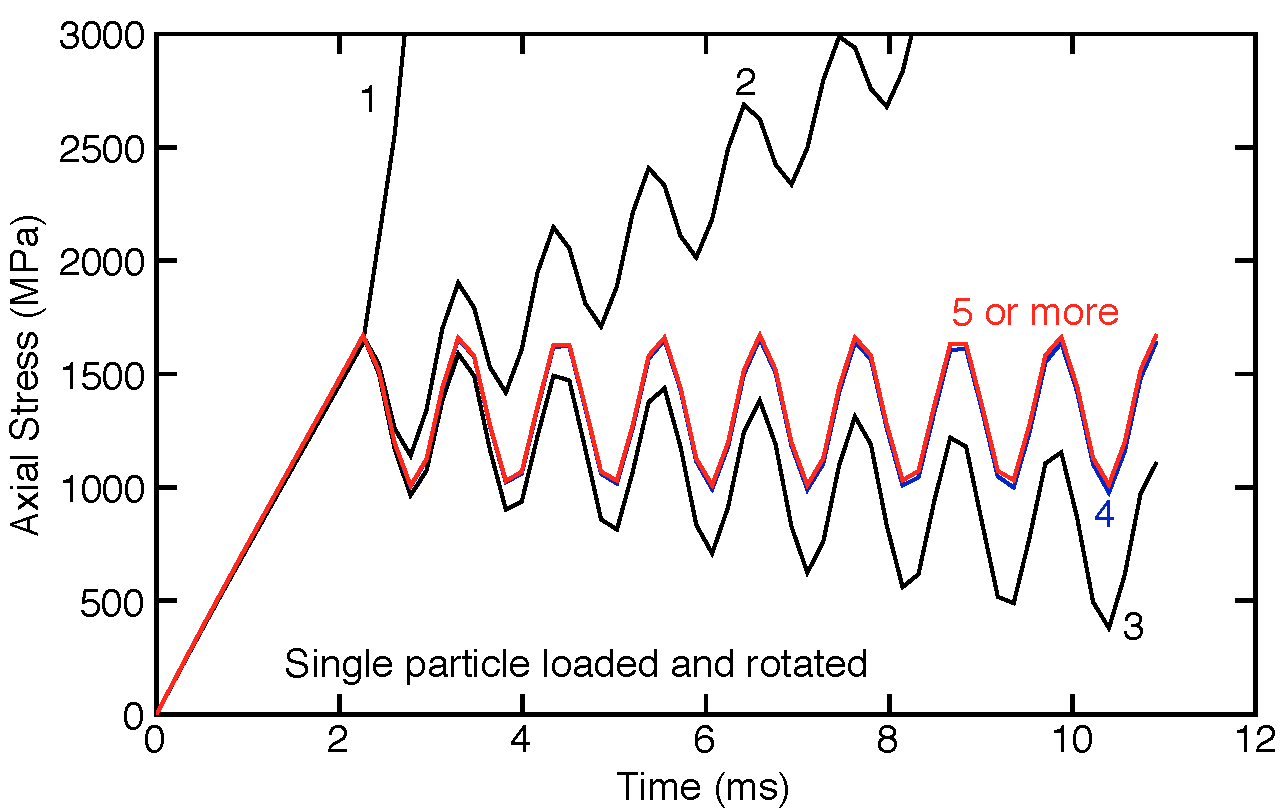
\includegraphics[width=5in]{IncrementalDef}
\caption{Calculation for a single particle loaded in tension, held, and then rotated. The different curves show $k_{max}$ or the number of terms used to expand the matrix exponential in the incremental deformation gradient.}
\label{dFCalc}
\end{center}
\end{figure}


\section{Hyperelastic 1D Membrane in a 2D Simulation}

A membrane in a 2D simulation is a 1D path through the object (this notes are plane stress and plane strain only and will need to be updated for axisymnetry). Imagine a coordinate system with the fiber direction of the membrane initially along the $x$ axis and the thickness direction along the $y$ axis. In membrane models, it is assumed there is no shear deformation in the plane of the membrane --- it has only stretches in fiber direction and thickness directions. As a result, the general deformation gradient is:

\begin{equation}
   \F = \left(\begin{array}{ccc}
          \lambda_1 \cos\theta & \lambda_2 \sin\theta & 0   \\
         -\lambda_1 \sin\theta  & \lambda_2 \cos\theta & 0   \\
        0 & 0 & \lambda_3
        \end{array}\right) = \left(\begin{array}{ccc}
         \cos\theta &  \sin\theta & 0   \\
         - \sin\theta  &  \cos\theta & 0   \\
        0 & 0 & 1
        \end{array}\right) \left(\begin{array}{ccc}
          \lambda_1 & 0 & 0   \\
         0  & \lambda_2  & 0   \\
        0 & 0 & \lambda_3
        \end{array}\right) = \tens{R}[\lambda]
\end{equation}
where $\lambda_i$ are stretches in three orthogonal membrane directions (and they remain orthogonal) and $\theta$ is the clockwise rotation of the current fiber direction from the global, positive $x$ axis direction. The first and second columns are vectors along the current fiber and thickness directions, respectively.

In an MPM time step, the membrane constitutive law will be provided an incremental deformation gradient, $\dF$ (as calculated above), but in general this deformation will not be compatible with a membrane deformation with zero shear. Instead, $\dF$ is just used to find new fiber vector:
\begin{equation}
   \vec{m} = (\dF_{11}\tens{F}_{11} + \dF_{12}\tens{F}_{21},\dF_{21}\tens{F}_{11} + \dF_{22}\tens{F}_{21})
\end{equation}
The magnitude of this vector is the new fiber stretch: $\lambda_1=||\vec{m}||$. A specific membrane material model should calculations $\lambda_2$ and $\lambda_3$ and then update the particle's deformation gradient to be:

\begin{equation}
   \F = \left(\begin{array}{ccc}
          m_x & -{\lambda_2\over\lambda_1}m_y  & 0   \\
          m_y  & {\lambda_2\over\lambda_1}m_x & 0   \\
        0 & 0 & \lambda_3
        \end{array}\right)
\end{equation}

For stresses and energy, membrane material classes find Kirchhoff stress in the unrotated membrane coordinates (which should only need the three $\lambda_i$ stretches and $\omega$). These stresses are rotated to the MPM coordinates:
\begin{equation}
    \tens\tau =  \tens{R} \tens{\tau} \tens{R}^T =  \tens{R}[\lambda]\bigl([\lambda]^{-1} \tens{\sigma}[\lambda]^{-T}\bigr)[\lambda]^T\tens{R}^T =  \F \tens{S} \F^T
\end{equation}
where $\F$ is the updated membrane deformation gradient on the particle and $\tens{S}$ is the second Poila-Kirchoff stress in the mebrane coordinates. The second Poila-Kirchoff stress will only have non-zero $\tens{S}_{11}$, $\tens{S}_{12}$, and $\tens{S}_{22}$ and it is found from $\tens{S} =  [\lambda]^{-1} \tens{\tau}[\lambda]^{-T}$ or $S_{11} = \tau_{11}/\lambda_1^2$.

Work and residual energy \hyperref[EnergyUpdates]{updates} can be done in the membrane coordinates:
\begin{equation}
         dw = \tau_{11} du_{11} \qquad {\rm and}\qquad  dw_{res} = \tau_{11} du_{11}^{res} + \tau_{33} du_{33}^{res}
\end{equation}
where $du_{11}$ is element of the displacement gradient for this step and $du_{res}^{ii}$ is incremental residual strain for this step. The displacement gradient can be found from the effective membrane incremental deformation gradient:
\begin{equation}
      \dF_{m} = \exp(\nabla \vec u) = \left(\begin{array}{ccc} {\lambda_1\over \lambda_1^{(n-1)}} & 0 & 0 \\
                                                0 & {\lambda_2\over \lambda_2^{(n-1)}} & 0 \\
                                                 0 & 0 & {\lambda_2\over \lambda_2^{(n-1)}}
                 \end{array}\right)    \quad {\rm or}\quad  du_{11} =  \ln {\lambda_1\over \lambda_1^{(n-1)}}
\end{equation}
where $\lambda_1^{(n-1)}$ are the stretches at the start of the time step.

\section{Hyperelastic 2D Membrane in a 3D Simulation}

A membrane in a 3D simulation is a 2D surface through the object. Imagine a coordinate system with the two fiber directions of the membrane initially along the $x$ and $y$ axes and the thickness direction along the $z$ axis. In membrane models, it is assumed the normal and shear stresses in the thickness direction of the membrane are zero --- the membrane has only stretches and shear in the plane defined by the two fiber directions. As a result, the general deformation gradient can be written as:

\begin{equation}
   \F = \tens{R}\left(\begin{array}{ccc}
          \lambda_1  & \lambda_2 \cos\omega & 0   \\
         0  & \lambda_2 \sin\omega & 0   \\
        0 & 0 & \lambda_3
        \end{array}\right)   = \tens{R}[\lambda\omega]
\end{equation}
where $\lambda_i$ are stretches in three initially orthogonal membrane directions and $\omega$ is the angle between the deformed, in-plane fiber directions. The rotation matrix $\tens{R}$ rotates the positive $x$ axis to the corresponding fiber axis in the deformed membrane.

In an MPM time step, the membrane constitutive law will be provided an incremental deformation gradient, $\dF$ (as calculated \hyperref[IDG]{above}), but in general this deformation will not be compatible with a membrane deformation where thickness direction should have stretch only and zero shear. Instead, $\dF$ is just used to find new fiber vectors from the first two columns of $\dF\cdot\F$. If these deformed vectors are $\vec{m_1}$ and $\vec{m_2}$ then the key deformation terms are:
\begin{equation}
     \lambda_1 = ||\vec{m_1}||, \quad \lambda_2 = ||\vec{m_2}||, \quad \cos\omega = {\vec{m_1}\cdot\vec{m_2}\over \lambda_1 \lambda_2},
     \quad {\rm and} \quad \sin\omega = {||\vec{m_1}\times\vec{m_2}||\over \lambda_1 \lambda_2}
\end{equation}
A specific membrane material model should calculate $\lambda_3$ for the thickness direction (to get zero thickness stress). The particle  deformation gradient is updated with $\vec{m_1}$, $\vec{m_2}$ left intact as first two columns, but the third column of the provisional $\dF\cdot\F$ is changed to be $\lambda_3(\vec{m_1}\times\vec{m_2})/(\lambda_1\lambda_2)$. In this approach, the membrane normal vector remains normal to both $\vec{m_1}$ and $\vec{m_2}$.

For stresses and energy, membrane material classes finds Kirchhoff stress ($\tens{\tau}$) in the unrotated membrane coordinates (which should only need the three $\lambda_i$ stretches and $\omega$). These stresses are rotated to the MPM coordinates:
\begin{equation}
    \tens\tau\ ({\rm MPM}) = \tens{R} \tens{\tau} \tens{R}^T =  \tens{R}[\lambda\omega]\bigl([\lambda\omega]^{-1} \tens{\tau}[\lambda\omega]^{-T}\bigr)[\lambda\omega]^T\tens{R}^T =  \F \tens{S} \F^T
\end{equation}
where $\F$ is the updated membrane deformation gradient on the particle and $\tens{S}$ is the second Poila-Kirchoff stress in the membrane coordinates. The second Poila-Kirchoff stress will only have non-zero $\tens{S}_{11}$, $\tens{S}_{12}$, and $\tens{S}_{22}$ and it is found from $\tens{S} =  [\lambda\omega]^{-1} \tens{\tau}[\lambda\omega]^{-T}$ or:
\begin{equation}
   \tens{S} = \left(\begin{array}{ccc}
          {1\over\lambda_1}  & -{ \cot\omega\over \lambda_1} & 0   \\
         0  & {1\over \lambda_2 \sin\omega} & 0   \\
        0 & 0 & {1\over\lambda_3}
        \end{array}\right)\left(\begin{array}{ccc}
          \tau_{11}  & \tau_{12} & 0   \\
         \tau_{12}  & \tau_{y22} & 0   \\
        0 & 0 & 0
        \end{array}\right)\left(\begin{array}{ccc}
          {1\over\lambda_1}  & 0 & 0   \\
         -{ \cot\omega\over \lambda_1}  & {1\over \lambda_2 \sin\omega} & 0   \\
        0 & 0 & {1\over\lambda_3}
        \end{array}\right)
\end{equation}
The result is
\begin{equation}
   \tens{S} = \left(\begin{array}{ccc}
          {1\over\lambda_1}  & -{ \cot\omega\over \lambda_1} & 0   \\
         0  & {1\over \lambda_2 \sin\omega} & 0   \\
        0 & 0 & {1\over\lambda_3}
        \end{array}\right)\left(\begin{array}{ccc}
          {\tau_{11}\over\lambda_1} - {\tau_{12}\cot\omega\over \lambda_1} & {\tau_{12}\over \lambda_2 \sin\omega} & 0   \\
         {\tau_{12}\over\lambda_1} - {\tau_{22}\cot\omega\over \lambda_1}  & {\tau_{22}\over \lambda_2 \sin\omega} & 0   \\
        0 & 0 & 0
        \end{array}\right)
\end{equation}
which simplifies to
\begin{eqnarray}
   S_{11} & = & {1\over\lambda_1^2}\left(\tau_{11} - 2\tau_{12}\cot\omega 
                          + \tau_{22}\cot^2\omega\right) \\
   S_{22} & = & {\tau_{22}\over\lambda_2^2\sin^2\omega} \\
   S_{12} & = & {(\tau_{12}-\tau_{22}\cot\omega)\over \lambda_1\lambda_2 \sin\omega}
\end{eqnarray}
These can be inverted to
\begin{eqnarray}
  \tau_{11} & = & S_{11}\lambda_1^2 + 2 S_{12}\lambda_1\lambda_2\cos\omega + S_{22}\lambda_2^2\cos^2\omega \\
   \tau_{22} & = & S_{22}\lambda_2^2\sin^2\omega \\
   \tau_{12} & = & S_{12}\lambda_1\lambda_2\sin\omega + S_{22}\lambda_2^2\cos\omega\sin\omega
\end{eqnarray}

The membrane deformation (or $[\lambda\omega]$) is tracked on the particle in the plastic strain. Work and residual energy \hyperref[EnergyUpdates]{updates} can be done in the membrane coordinates:
\begin{eqnarray}
         dw & = & \tau_{11} du_{11} + \tau_{12}(du_{12}+du_{21}) + \tau_{22} du_{22}  \label{memwork} \\
         dw_{res} & = & \tau_{11} du_{11}^{res} + \tau_{12} (du_{12}^{res}+(du_{12}^{res}) 
                  + \tau_{22} du_{22}^{res}
\end{eqnarray}
where $du_{ij}$ are elements of the displacement gradient for this step and $du_{res}^{ij}$ are incremental residual strains for this step. The displacement gradient can be found from the effective membrane incremental deformation gradient, which is defined by $[\lambda\omega] = \dF_{m}  [\lambda\omega]_{n-1}$ giving
\begin{eqnarray}
      \dF_{m} = \exp(\nabla \vec u) = [\lambda\omega][\lambda\omega]_{n-1}^{-1}
            & = & \left(\begin{array}{ccc} \lambda_1 & \lambda_2\cos\omega & 0 \\
                                                0 & \lambda_2\sin\omega & 0 \\
                                                 0 & 0 & \lambda_3
                 \end{array}\right)\left(\begin{array}{ccc} {1\over M_{11}} & -{M_{12}\over M_{11}M_{22}} & 0 \\
                                       0 & {1\over M_{22}} & 0 \\
                                        0 & 0 & {1\over M_{33}}
                 \end{array}\right) \\
         & = & \left(\begin{array}{ccc} {\lambda_1\over M_{11}} & {\lambda_2\cos\omega\over M_{22}} 
                                                                -{M_{12}\lambda_1\over M_{11}M_{22}}& 0 \\
                                                0 & {\lambda_2\sin\omega\over M_{22}} & 0 \\
                                                 0 & 0 & {\lambda_3\over M_{33}}
                 \end{array}\right)
\end{eqnarray}
where $[\lambda\omega]_{n-1}$ is the membrane-coordinates deformation gradient at the start of the time step and $M_{ij}$ are elements of $[\lambda\omega]_{n-1}$. Assuming that gradient of the displacement vector has non-zero elements the same places as $\dF_{m}$, the exponential can be evaluated:
\begin{equation}
        \exp(\nabla \vec u) = \left(\begin{array}{ccc} e^{du_{11}} & {du_{12}\over du_{11}}\left(e^{du_{22}}-e^{du_{11}}\right) & 0 \\
                                       0 & e^{du_{22}} & 0 \\
                                        0 & 0 & e^{du_{33}}
                 \end{array}\right)\
\end{equation}
From which
\begin{eqnarray}
   du_{11} & = &  \ln {\lambda_1\over M_{11}} \\
   du_{22} & = &  \ln {\lambda_2\sin\omega\over M_{22}} \\
   du_{33} & = &  \ln {\lambda_3\over M_{33}} \\
   du_{12} & = &   \ln {\lambda_1\over M_{11}} {{\lambda_2\cos\omega\over M_{22}}-{M_{12}\lambda_1\over M_{11}M_{22}} \over
                        {\lambda_2\sin\omega\over M_{22}} - {\lambda_1\over M_{11}} }
\end{eqnarray}

Alternatively, the incremental work can be written as
\begin{equation}
     dw = \S\cdot \dot\E \thinspace dt = {1\over 2}\S\cdot \dot\C \thinspace dt
\end{equation}
where $\E$ is Green-Lagrange strain. Evaluating $\dot\C$ and using $\dot\F = \nabla v\F$ gives
\begin{equation}
    \dot\C = \dot\F^T\F+\F^T\dot\F = \F^T\bigl(\nabla v^T+\nabla v)\F
\end{equation}
The energy increment (using tensors in the membrane coordinates) becomes
\begin{equation}
     dw = \S\cdot[\lambda\omega]^T\left({1\over 2}\bigl(\nabla u^T+\nabla u)\right)[\lambda\omega]
\end{equation}
Expansion of this expression is identical to Eq.~(\ref{memwork}) (as it must be).


\section{Membrane Material Tasks\label{MMT}}

Much of the work for membrane model is done by the {\tt MemPoint2D.cpp}, {\tt MemPointAS.cpp} and {\tt MemPoint3D.cpp} classes. These classes do the following tasks:

\begin{enumerate}
\item Use $\dF$ to find $\lambda_1$ (2D), $\lambda_1$ and $\lambda_3$ (AS), or $\lambda_1$, $\lambda_2$, and $\omega$ (3D).
\item Call the material class, which will complete these calculations
\begin{enumerate}
\item For 2D and axisymmetric simulations, find $\lambda_2$, $\lambda_3$ (plane stress only), $\tau_{11}$ and $\tau_{33} = \tau_{zz}$. For 3D simulations, find $\lambda_3$, $\tau_{11}$, $\tau_{12}$, and $\tau_{22}$ ($\tau_{33}$ is zero, which may be used in the material model when finding the other quantities).
\item Alternatively, a membrane material can find $S_{ij}$ in the membrane instead of $\tau_{ij}$ and then set {\tt isPoila} variable to {\tt true}.
\item Call method to update residual energy (it is done in the material to be able to handle anisotropic materials).
\item Call method to track temperature, entropy, and heat on the particle.
\end{enumerate}
\item Find $du_{ij}$ and increment work energy
\item Store $[\lambda]$ (2D) or $[\lambda\omega]$ (3D) in the particle plastic strain
\item Update $\F$ on the particle
\item Rotate membrane stress to MPM coordinates and store on the particle stresses.
\end{enumerate}

The material class works in a simplified deformation system. In 2D plane stress simulations with fiber stretch $\lambda_1$, $J=\lambda_1\lambda_2\lambda_3$ and $\lambda_2=\lambda_3 = \sqrt{J/\lambda_1}$ (assuming isotropic). The left Cauchy-Green deformation tensor in the membrane coordinates has non-zero elements $\tens{B}_{11} = \lambda_1^2$ and $\tens{B}_{22} = \tens{B}_{33}=J/\lambda_1$.

In 2D plane strain (or axisymmetric) simulations with fiber stretch $\lambda_1$, $J=\lambda_1\lambda_2\lambda_3$, $\lambda_3=1$ (plane strain) or is an input $\lambda_3$ (axisymmetric), and $\lambda_2=J/(\lambda_1\lambda_3)$. The left Cauchy-Green deformation tensor in the membrane coordinates has non-zero elements $\tens{B}_{11} = \lambda_1^2$, $\tens{B}_{22} = J^2/(\lambda_1^2\lambda_3^2)$, and $\tens{B}_{33}=\lambda_3^2$.

In 3D simulations with fiber stretches $\lambda_1$ and $\lambda_2$, $J=\lambda_1\lambda_2\lambda_3\sin\omega$, and $\lambda_3=J/(\lambda_1\lambda_2\sin\omega)$. The left Cauchy-Green deformation tensor in the membrane coordinates is
\begin{equation}
   \B = \F\F^T =  \left(\begin{array}{ccc}
          \lambda_1^2 + \lambda_2^2\cos^2\omega  & \lambda_2^2\sin\omega\cos\omega & 0   \\
         \lambda_2^2\sin\omega\cos\omega  & \lambda_2^2 \sin^2\omega & 0   \\
        0 & 0 & \lambda_3^2
        \end{array}\right)
\end{equation}
and the right Cauchy-Green deformation tensor in the membrane coordinates is
\begin{equation}
   \C = \F^T\F =  \left(\begin{array}{ccc}
          \lambda_1^2   & \lambda_1\lambda_2\cos\omega & 0   \\
         \lambda_1\lambda_2\cos\omega  & \lambda_2^2  & 0   \\
        0 & 0 & \lambda_3^2
        \end{array}\right)
\end{equation}

Finally, in {\tt NairnMPM}, the membrane deformation matrix ($[\lambda]$ or $[\lambda\omega]$), is tracked on the particle using the particle's plastic strain. Note that other Hyperelastic materials track $\B$ in the plastic strain and hyperelastic, plasticity materials track the elastic $\B$; plastic membranes will need an alternate method to store elastic deformation information.

\section{Isotopic, Hyperelastic Materials}

Isotropic, hyperelastic materials can be derived by defining an energy function in terms of invariants of $\F$ or other large-strain tensors. One approach is based on invariants of the left, Cauchy-Green tensor:
\begin{eqnarray}
          I_1 & = & {\rm Tr}(\B) = B_{11} + B_{22} + B_{33} = \lambda_1^2 +  \lambda_2^2 + \lambda_3^2 \\
          I_2 & = & {1\over2}\left(I_1^2 - \B\cdot \B\right) = \lambda_1^2\lambda_2^2 + \lambda_1^2\lambda_3^2 + \lambda_1^2\lambda_3^2\\
          I_3 & = & {\rm det}(\B) = J^2 = \lambda_1^2\lambda_2^2\lambda_3^2
\end{eqnarray}
where $\lambda_i$ are the principle stretches of the deformation.
Sometimes modified invariants are used instead as $\overline{I_1} = I_1/J^{2/3}$ and $\overline{I_2} = I_2/J^{4/3}$. Next the strain energy is written as a function of these invariants, with the common forms being $W(I_1,I_2,J)$, $W(\overline{I_1},\overline{I_2},J)$ and $W( \lambda_1,\lambda_2,\lambda_3)$. In these three forms, the Cauchy stress can be found from
\begin{eqnarray}
   \tens\sigma & = & {\partial W\over \partial J}\I + {2\over J}\left[ {\partial W\over \partial I_1}\B
                                             + {\partial W\over \partial I_2}\left(I_1\B- \B^2\right)
                                            \right]      \\
   \tens\sigma & = & {\partial W\over \partial J}\I + 2\left[ {1\over J^{5/3}}
                           {\partial W\over \partial \overline{I_1}}\left(\B -  {I_1\over 3}\I\right)
                           + {1\over J^{7/3}}{\partial W\over \partial \overline{I_2}}\left( I_1 \B- \B^2 - {2I_2\over 3}\I  \right)
                             \right] \\
   \tens\sigma & = & \sum_k {\lambda_k\over J} {\partial W\over\partial \lambda_k} \vec b_k\otimes\vec b_k
\end{eqnarray}
where $\vec b_k$ is the eigenvector of $\B$ associated with eigenvalue $\lambda_k^2$.
Because $\B$ is symmetric (and therefore ${\rm Tr}(\B^2) = \B\cdot\B$ and ${\rm Tr}(I_1\B-\B^2)=I_1^2-\B\cdot\B = 2I_2$), the second version can be written
\begin{equation}
           \tens\sigma = {\partial W\over \partial J}\I + 2\left[ {1\over J^{5/3}}
                                           {\partial W\over \partial \overline{I_1}}{\rm dev}(\B)
                                        + {1\over J^{7/3}}{\partial W\over \partial \overline{I_2}}{\rm dev}( I_1 \B- \B^2)
                                           \right]
\end{equation}
The pressure ($P = -{\rm Tr}(\tens\sigma)/3$) can be found (making use of ${\rm Tr}({\rm dev}(\cdot))=0$) from three results as
\begin{eqnarray}
   P & = & -{\partial W\over \partial J} - {2\over 3J}\left[ {\partial W\over \partial I_1}I_1  + {\partial W\over \partial I_2}2I_2   \right]      \\
   P & = & - {\partial W\over \partial J} \\
   P & = &  -{1\over 3}\sum_k {\lambda_k\over J} {\partial W\over\partial \lambda_k}
\end{eqnarray}
with the last one assuming orthonormal eigenvectors.
Thus the deviatoric Cauchy stresses are ($\dev = \tens\sigma + P\I$):
\begin{eqnarray}
   \dev & = &  {2\over J}\left[ {\partial W\over \partial I_1}{\rm dev}(\B)
                                             + {\partial W\over \partial I_2}{\rm dev}\left(I_1\B- \B^2\right)
                                            \right]      \\
   \dev & = &  {2\over J}\left[ {1\over J^{2/3}}{\partial W\over \partial \overline{I_1}}{\rm dev}(\B)
                                        + {1\over J^{4/3}}{\partial W\over \partial \overline{I_2}}{\rm dev}( I_1 \B- \B^2)
                                           \right] \\
   \dev & = &  \sum_k {\lambda_k\over J} {\partial W\over\partial \lambda_k} {\rm dev}(\vec b_k\otimes\vec b_k)
\end{eqnarray}

\section{Mooney-Rivlin Material\label{MRM}}

The Mooney-Rivilin material is an isotropic, elastic, hyperelastic material. It's stresses are based on a strain energy function that is assumed to be
\begin{equation}
W(\overline{I_1},\overline{I_2},J)= {G_1\over2}\left(\overline{I_1}-3\right) + {G_2\over2}\left(\overline{I_2}-3\right) + {K\over2}\left(J-1\right)^2
\end{equation}
where $G_1$, $G_2$, and $K$ are material properties.
For low strains, this material is equivalent for a linear elastic, isotropic material with shear modulus $G_1+G_2$ and bulk modulus $K$. If $G_2=0$, the material is one form or a neo-Hookean material (another form is given \hyperref[NHM]{below}). See below for alternate compressibility terms. Some hyperelastic rubber models assume incompressible materials, which corresponds to $K\to\infty$; such models do not work in dynamic code (because wave speed is infinite), although they can be used in membranes.

The Cauchy (or true stress) is found by differentiating the strain energy to get
\begin{equation}
     \tens\sigma = {G_1\over J^{5/3}}\left(\B - {I_1\over3}\I\right)
                     +  {G_2\over J^{7/3}}\left(I_1\B - \B^2 - {2I_2\over3}\I\right)   + K(J-1)\I
\end{equation}
The stress components can be divided into pressure, $P$, and deviatoric stress, $\dev = \tens\sigma+P\I$, which explicitly evaluate to:
\begin{eqnarray}
      P & = & -K (J-1) \\
     s_{xx} & = & G_1{2B_{xx}-B_{yy}-B_{zz}\over 3J^{5/3}} + G_2{B_{xx}(B_{yy}+B_{zz})-2B_{yy}B_{zz}-B_{xy}^2-B_{xz}^2+2B_{yz}^2\over 3J^{7/3} }\\
      s_{yy} & = & G_1{2B_{yy}-B_{xx}-B_{zz}\over 3J^{5/3}} + G_2{B_{yy}(B_{xx}+B_{zz})-2B_{xx}B_{zz}-B_{xy}^2+2B_{xz}^2-B_{yz}^2\over 3J^{7/3} }\\
      s_{zz} & = &  G_1{2B_{zz}-B_{xx}-B_{yy}\over 3J^{5/3}} + G_2{B_{zz}(B_{xx}+B_{yy})-2B_{xx}B_{yy}+2B_{xy}^2-B_{xz}^2-B_{yz}^2\over 3J^{7/3} }\\
      s_{xy} & = &  G_1{B_{xy}\over J^{5/3}} + G_2{B_{zz}B_{xy}-B_{xz}B_{yz}\over J^{7/3}}\\
      s_{xz} & = & G_1{B_{xz}\over J^{5/3}} + G_2{B_{yy}B_{xz}-B_{xy}B_{yz}\over J^{7/3}}\\
      s_{yz} & = & G_1{B_{yz}\over J^{5/3}} + G_2{B_{xx}B_{yz}-B_{xy}B_{xz}\over J^{7/3}}
\end{eqnarray}

\subsection{Plane Strain, Plane Stress, and Axisymmetric Analysis}

For 2D analyses, $F_{xz}=F_{yz}=F_{zx}=F_{zy}=0$, which leads to zero for corresponding terms in $\B$. The resulting stresses are $ P = -K (J-1)$ , $s_{xz}=s_{yz}=0$, and
\begin{eqnarray}
      s_{xx} & = &  G_1{2B_{xx}-B_{yy}-B_{zz}\over 3J^{5/3}}  
                    + G_2{B_{xx}(B_{yy}+B_{zz})-2B_{yy}B_{zz}-B_{xy}^2\over 3J^{7/3} }\\
      s_{yy} & = &  G_1{2B_{yy}-B_{xx}-B_{zz}\over 3J^{5/3}}   
                     + G_2{B_{yy}(B_{xx}+B_{zz})-2B_{xx}B_{zz}-B_{xy}^2\over 3J^{7/3} }\\
      s_{zz} & = &   G_1{2B_{zz}-B_{xx}-B_{yy}\over 3J^{5/3}}   
                     + G_2{B_{zz}(B_{xx}+B_{yy})-2B_{xx}B_{yy}+2B_{xy}^2\over 3J^{7/3} }\\
      s_{xy} & = &  G_1{B_{xy}\over J^{5/3}} + G_2{B_{zz}B_{xy}\over J^{7/3}}
\end{eqnarray}
For plane strain analysis $B_{zz}=1$. For axisymmetric analysis, $B_{zz}$ is provided by the input deformation. For plane stress analysis, one has to solve numerically for $B_{zz}$ to get $\s{zz}=0$ or $s_{zz}=P$ and then use that result to find $\e{zz}$ and other stresses.

In the presence of residual stresses (see \hyperref[HyperRes]{details below}), $\s{zz}=0$ is found by solving $f=0$ where
\begin{equation}
       f = -3J_{res}J_{eff}^2 P(J_{eff}) + G_1 J^{1/3} (2B_{zz}-\alpha_1)+ {G_2\over J^{1/3} }\bigl( B_{zz}\alpha_1-2\alpha_2\bigr)
\end{equation}
where $P(J_{eff})$ is the \hyperref[PTerms]{pressure model} used, $\alpha_1 = B_{xx}+B_{yy}$, $\alpha_2 = B_{xx}B_{yy}-B_{xy}^2$, $J^2 = {\rm det}(\B) = B_{zz}\alpha_2$, and $J_{eff}=J/J_{res}$. More explicitly in $B_{zz}$, the function is
\begin{equation}
       f = -3J_{res}J_{eff}^2 P(J_{eff})+ G_1 B_{zz}^{1/6} \alpha_2^{1/6}(2B_{zz}-\alpha_1)+ {G_2\over B_{zz}^{1/6} \alpha_2^{1/6} }\bigl( B_{zz}\alpha_1-2\alpha_2\bigr)
\end{equation}
For more efficient Newton's method, we need
\begin{equation}
       {df\over dB_{zz}} = -3J_{res}{d \left(J_{eff}^2 P(J_{eff})\right)\over dJ_{eff}}{dJ_{eff}\over dB_{zz}} + {G_1J^{1/3}(14B_{zz}- \alpha_1)\over 6B_{zz}} 
               + {G_2(5\alpha_1B_{zz}+2\alpha_2)\over  6 B_{zz}J^{1/3}} 
\end{equation}
where $J_{eff} = \sqrt{B_{zz}\alpha_2}/J_{res}$ and $B_{zz}(dJ_{eff}/ dB_{zz}) = \sqrt{B_{zz}\alpha_2}/(2J_{res})$. The first term simplifies to:
\begin{equation}
       {df\over dB_{zz}} = -{3J\over 2B_{zz}}{d \left(J_{eff}^2 P(J_{eff})\right)\over dJ_{eff}} + {G_1J^{1/3}(14B_{zz}- \alpha_1)\over 6B_{zz}} 
               + {G_2(5\alpha_1B_{zz}+2\alpha_2)\over  6 B_{zz}J^{1/3}} 
\end{equation}
For the pressure term above
\begin{equation}
      -{3J\over 2B_{zz}}{d \left(J_{eff}^2 P(J_{eff})\right)\over dJ_{eff}} = {3 J \over 2B_{zz}}KJ_{eff}(3J_{eff}-2)
\end{equation}
Other \hyperref[PTerms]{pressure models} are given below.

\subsection{Dealing with Thermal and Moisture Strains\label{HyperRes}}

To handle thermal and moisture strains the deformation is divided into two steps. The first is free expansion to the new stress free volume and then deformation to the final volume. The total deformation will be
\begin{equation}
      \F = \F^* \F^{res} = \F^* \lambda_{res}\I
\end{equation}
where $\lambda_{res}$ is total extension due to free thermal and moisture expansion:
\begin{equation}
    \lambda_{res} = \exp( \alpha\Delta T + \beta \Delta c) \approx  1 +\alpha\Delta T + \beta \Delta c
\end{equation}
where the approximation is for small $\Delta T$ and $\Delta x$.
The stresses and energy, however, should be found using $\F^*$ instead of $\F$, where $\F^*$ is now deformation from the current free expansion volume instead of from the initial volume. The net effects are $\F^* = \F/\lambda_{res}$, $J_{eff} = |\F^*| = J/\lambda_{res}^3$, and $\B_{eff} = \B/\lambda_{res}^2$. In the above equations, the Cauchy stress is found by replacing $J$ with $J_{eff}$ in the \hyperref[PTerms]{pressure model} and by multiplying all shear terms by $J_{res} = \lambda_{res}^3$, or explicitly by three equivalent forms:
\begin{eqnarray}
     \tens\sigma & = & {\Jres G_1\over J^{5/3}}\left(\B - {I_1\over3}\I\right)
                     +  {\Jres G_2\over J^{7/3}}\left(I_1\B - \B^2 - {2I_2\over3}\I\right)  - P(\Jeff)\I    \\
     \tens\sigma & = & {G_1\over \Jeff J^{2/3}}\left(\B - {I_1\over3}\I\right)
                     +  {G_2\over \Jeff J^{4/3}}\left(I_1\B - \B^2 - {2I_2\over3}\I\right) -  P(\Jeff)\I    \\
     \tens\sigma & = & {G_1\over \Jres^{2/3}\Jeff^{5/3}}\left(\B - {I_1\over3}\I\right)
                     +  {G_2\over \Jres^{4/3}\Jeff^{7/3}}\left(I_1\B - \B^2 - {2I_2\over3}\I\right) -  P(\Jeff)\I
\end{eqnarray}

These results reduce to the proper low-strain thermoelastic relation at small strain. In this limit
\begin{equation}
   \B \approx \I + 2\tens{\varepsilon}, \quad I_1 \approx 3 + 2{\rm Tr}(\tens\varepsilon), 
         \quad \B^2\approx \I + 2\tens\varepsilon, \quad J \approx 1 + {\rm Tr}(\tens\varepsilon), \quad {\rm and}
         \quad {1\over\Jres} \approx 1-3\alpha\Delta T 
\end{equation}
leading to
\begin{equation}
     \tens\sigma =G_1\left(2\tens{\varepsilon} - {2\over3}{\rm Tr}(\tens\varepsilon)\I\right)
                 +  G_2\left(2\tens{\varepsilon} 
                      + \left(I_1\left(1-{I_1\over3}\right)-1+{\B\cdot\B\over3}\right)\I\right) 
                       + K({\rm Tr}(\tens\varepsilon)-3\alpha\Delta T) \I
\end{equation}
Using $\B\cdot\B \approx 3 + 4{\rm Tr}(\tens\varepsilon)$ leads to
\begin{eqnarray}
     \tens\sigma & = & (G_1+G_2)\left(2\tens{\varepsilon} - {2\over3}{\rm Tr}(\tens\varepsilon)\I\right)
                       + K({\rm Tr}(\tens\varepsilon)-3\alpha\Delta T)\I   \\
         & = &   \left[\left(K-{2\over3}(G_1+G_2)\right){\rm Tr}(\tens\varepsilon) - 3K\alpha\Delta T\right]\I
                        + 2(G_1+G_2)\tens{\varepsilon}
\end{eqnarray}
which is the expected result where $G_1+G_2$ is the low-strain shear modulus.


When doing incremental deformation, $\F_{k+1} = \dF\cdot\F_k$ and incremental volume ratio is $dJ = |\dF| = V_{k+1}/ V_k$, but $J_{eff}$ is $V/V_{sf}$ where $V_{sf}$ is the current stress free volume. For incremental deformation, $J_{k+1} = dJ J_k$, but we really want to increment $J_{eff,k+1} = dJ_{eff}J_{eff,k}$, which is\begin{equation}
     J_{eff,k+1} = {V_{k+1}\over V_{sf,k+1}} = {V_{k+1}\over V_{k}}{V_{sf,k}\over V_{sf,k+1}} {V_{k}\over V_{sf,k}}
             = {V_{k+1}\over V_{k}}{V_{sf,k}\over V_{sf,k+1}} J_{eff,k} = dJ_{eff}J_{eff,k}
\end{equation}
which implies that
\begin{equation}
      dJ_{eff} = {V_{k+1}\over V_{k}}{V_{sf,k}\over V_{sf,k+1}} = dJ/d\lambda_{res}^3
\end{equation}
where
\begin{equation}
    d\lambda_{res} = \exp(\alpha dT + \beta dc) \approx 1 + \alpha dT + \beta dc
\end{equation}
where $dT$ and $dc$ are temperature and concentration changes on the current time step.

\subsection{Alternate Bulk Modulus Term\label{PTerms}}

Besides the dilation energy term used above of
\begin{equation}
W = {K\over2}(J-1)^2  \qquad{\rm with}\qquad P = -K (J-1),
\end{equation}
two alternative compressibility terms are:

\begin{equation}
W = {K\over2}(\ln J)^2  \qquad{\rm and}\qquad W = {K\over2}\left({1\over2}(J^2-1) - \ln J\right)
\end{equation}

\noindent which gives normal Cauchy pressure terms of
\begin{equation}
     P = -K {\ln J\over J}  \qquad{\rm and}\qquad P = - {K\over 2}\left(J-{1\over J}\right)
\end{equation}

\noindent Although these three compressibility terms show some significant differences when $J$ deviates significantly from 1, under most problems, $J$ will stay close to one. Two exceptions could be constrained compression or tension. Here, the only one that works well to very small or large $J$ is the second one above. This one correctly leads to inifinite positive stress as $J\to\infty$ and infinite negative stress as $J\to0$. This later one is the default for this material in {\tt NairnMPM}.

When implementing plane stress, the pressure term derivatives for these two new laws are:
\begin{eqnarray}
      {d(\Jeff^2 P(\Jeff))\over d\Jeff} & = & -K{d \left(J_{eff}\ln J_{eff}\right)\over dJ_{eff}} = -K(1+\ln J_{eff}) \\
      {d(\Jeff^2 P(\Jeff))\over d\Jeff} & = & -{K\over 2}{d \left(J_{eff}^3 - J_{eff}\right)\over dJ_{eff}} =  -{K\over 2}(3J_{eff}^2-1)
\end{eqnarray}

\subsection{Tangent Bulk Modulus}

The incremental bulk modulus is
\begin{equation}
   {1\over K(P)} = - {d\ln V\over dP} = - {d\ln \Jeff\over dP}  \qquad{\rm or} \qquad K = -\Jeff {dP\over d\Jeff}
\end{equation}
The various bulk moduli are (using $J$ for $\Jeff$):
\begin{eqnarray}
   P = -K_0(J-1) &\qquad{\rm gives}\qquad & K = K_0 J \\
   P = -K_0 {\ln J\over J} &\qquad{\rm gives}\qquad& K_0{1-\ln J \over J ^2}\\
   P = - {K_0\over 2}\left(J -{1\over J }\right) &\qquad{\rm gives}\qquad& K = {K_0\over 2}\left(J  + {1\over J }\right)
\end{eqnarray}

\subsection{Plane Stress Mooney-Rivlin Membrane}

Using the deformation state for \hyperref[MMT]{plane stress membrane} and defining $\lambda=\lambda_1)$ a Mooney-Rivlin material has the normal Cauchy stresses:
\begin{eqnarray}
      \sigma_{11} & = & -P(\Jeff) + 2\Jres G_1{\lambda^2-{J\over\lambda}\over 3J^{5/3}} + 2\Jres G_2{\lambda-{J\over\lambda^2}\over 3J^{4/3}} \\
      \sigma_{22} = \sigma_{33} & = & -P(\Jeff) +  \Jres G_1{{J\over\lambda}-\lambda^2\over 3J^{5/3}} + \Jres G_2{{J\over\lambda^2}-\lambda\over 3J^{4/3}}
\end{eqnarray}
where the $P(\Jeff)$ is the \hyperref[PTerms]{pressure model}. The stress state is found by numerically solving $\sigma_{22}=0$ for $J$ or solving:
\begin{equation}
	-P(\Jeff) =  \Jres G_1{\lambda^2-{J\over\lambda}\over 3J^{5/3}} + \Jres G_2{\lambda-{J\over\lambda^2}\over 3J^{4/3}}
\end{equation}
For Newton's method, solve $f=0$ for $J$ using
\begin{eqnarray}
	f & = & 3\Jres \Jeff^2 P(\Jeff) + (J^{1/3}G_1+J^{2/3}G_2)\left(\lambda^2-{J\over\lambda}\right) \\
	{df\over dJ} & = & 3 {d(\Jeff^2 P(\Jeff))\over d\Jeff} + {J^{1/3}G_1\over 3}\left({\lambda^2\over J}-{4\over\lambda}\right)
	+ {J^{2/3}G_2\over 3}\left({2\lambda\over J}-{5\over\lambda^2}\right)
\end{eqnarray}

Given this $J$, the final Kirchhoff stress results are
\begin{equation}
     \tau_{11} =  {1\over \Jeff}\left(J^{1/3}G_1 + {J^{2/3}G_2\over \lambda}\right)\left(\lambda^2-{J\over\lambda}\right) \quad{\rm and}\quad
     \tau_{33} = 0 
\end{equation}
and   $ \lambda_2 = \lambda_3 = \sqrt{J/\lambda}$.
Normally dynamic code cannot model an incompressible material, but an incompressible membrane material can be modeled by setting $J=\Jres$ and $\Jeff = 1$ or:
\begin{equation}
     \tau_{11} = \left(\Jres^{1/3}G_1 + {\Jres^{2/3}G_2\over \lambda}\right)\left(\lambda^2-{\Jres\over\lambda}\right) \quad{\rm and}\quad
     \tau_{33} = 0 
\end{equation}
and $ \lambda_2 = \lambda_3 = \sqrt{\Jres/\lambda}$.
Note that during free thermal expansion, $\Jres=\lambda^3$ and all stresses are zero.

\subsection{Plane Stress Mooney-Rivlin Membrane --- Alternate Approach}

In this alternate approach, the new fiber stretch is found by conserving the imposed incremental volume change, $dJ$, and then finding the new fiber stretch to keep the thickness stress equal to zero.

In 2D plane stress simulations with incremental fiber stretch $d\lambda$, $J = J_n=d\lambda d\lambda_2 d\lambda_3 J_{n-1}$ and $d\lambda_2=d\lambda_3 = \sqrt{dJ/d\lambda}$. The left Cauchy-Green deformation tensor current membrane coordinates has non-zero elements $\tens{B}_{11} = \lambda_n^2$, $\tens{B}_{22} = \tens{B}_{33}=J/\lambda_n$, where $\lambda_n = d\lambda\lambda$ is the new fiber stretch in the $n^{th}$ step. For a Mooney-Rivlin material (here neo-hookean only with $G_1=G$ and $G_2=0$) the normal Cauchy stresses are:
\begin{eqnarray}
      \sigma_{11} & = & -P(\Jeff) + 2\Jres G{\lambda_n^2-{J\over \lambda_n}\over 3J^{5/3}}  \\
      \sigma_{22} = \sigma_{33} & = & -P(\Jeff) +  \Jres G{{J\over \lambda_n}-\lambda_n^2\over 3J^{5/3}}
\end{eqnarray}
where the $P(\Jeff)$ is the \hyperref[PTerms]{pressure model}. The stress state is found by solving $\sigma_{yy}=0$ for $d\lambda=\lambda_n/\lambda_{n-1}$, which is a cubic equation:
\begin{equation}
	 \lambda_n^3+{3J^{2/3}\Jeff P(\Jeff)\over G} \lambda_n - J = 0
\end{equation}
This depressed cubic can be found analytically. When this approach was tried, the resulting membrane seemed too stiff and the stiffness was a strong function of the Poisson's ratio. This approach is not recommended for MPM membrane analysis.

\subsection{Plane Strain and Axisymmetric Mooney-Rivlin Membrane}

Using the deformation state for \hyperref[MMT]{plane strain or axiymmetric membranes} and defining $\lambda=\lambda_1$, a Mooney-Rivlin material has the normal Cauchy stresses:
\begin{eqnarray}
      \sigma_{11} & = & -P(\Jeff) + \Jres G_1{2\lambda^2-{J^2\over\lambda^2\lambda_3^2}-\lambda_3^2\over 3J^{5/3}} 
                                  + \Jres G_2{\lambda^2\lambda_3^2 + {J^2\over \lambda_3^2} -2{J^2\over\lambda^2}\over 3J^{7/3}} \\
      \sigma_{22} & = & -P(\Jeff) + \Jres G_1{2{J^2\over\lambda^2\lambda_3^2}-\lambda^2-\lambda_3^2\over 3J^{5/3}}
                                  + \Jres G_2{{J^2\over\lambda_3^2} + {J^2\over\lambda^2}-2\lambda^2\lambda_3^2\over 3J^{7/3}}  \\
      \sigma_{33} & = & -P(\Jeff) + \Jres G{2\lambda_3^2-\lambda^2-{J^2\over\lambda^2\lambda_3^2}\over 3J^{5/3}} 
                                  + \Jres G_2{\lambda^2\lambda_3^2 + {J^2\over\lambda^2}-2{J^2\over \lambda_3^2}\over 3J^{7/3}}
\end{eqnarray}
where the $P(\Jeff)$ is the \hyperref[PTerms]{pressure model}. The stress state is found by numerically solving $\sigma_{22}=0$ for $J$ or solving:
\begin{equation}
	-P(\Jeff) =  \Jres G_1{\lambda_3^2+\lambda^2-2{J^2\over\lambda^2\lambda_3^2}\over 3J^{5/3}} + 
	             \Jres G_2{2\lambda^2\lambda_3^2 - {J^2\over \lambda_3^2} - {J^2\over\lambda^2}\over 3J^{7/3}}
\end{equation}
For Newton's method, solve $f=0$ for $J$ using
\begin{eqnarray}
	f & = & 3 \Jres \Jeff^2 P(\Jeff) + J^{1/3} G_1\left(\lambda_3^2+\lambda^2-2{J^2\over\lambda^2\lambda_3^2}\right)
	                         + {G_2\over J^{1/3}}\left(2\lambda^2\lambda_3^2 - J^2\left({1\over \lambda_3^2}
	                         +{1\over\lambda^2}\right)\right)     \nonumber \\
	{df\over dJ} & = & 3 {d(\Jeff^2 P(\Jeff))\over d\Jeff} + {J^{1/3}G_1\over3}\left({\lambda_3^2+\lambda^2\over J}-{14J\over\lambda^2\lambda_3^2}\right)
	          - {G_2\over3J^{1/3}}\left({2\lambda^2\lambda_3^2\over J}+5J\left({1\over \lambda_3^2}+{1\over\lambda^2}\right)\right)
	          \nonumber \\
\end{eqnarray}

Given this $J$, the final Kirchhoff stress results are
\begin{eqnarray}
     \tau_{11} & = & {1\over \Jeff}\left(J^{1/3}G_1 + {G_2\lambda_3^2\over J^{1/3}}\right)
                       \left(\lambda^2-{J^2\over\lambda^2\lambda_3^2}\right) \\
     \tau_{33} & = & {1\over \Jeff}\left(J^{1/3}G_1 + {G_2\lambda^2\over J^{1/3}}\right)\left(\lambda_3^2-{J^2\over\lambda^2\lambda_3^2}\right)
\end{eqnarray}
and $\lambda_2 = J/(\lambda\lambda_3)$. Normally dynamic code cannot model an incompressible material, but a plane strain incompressible membrane material can be modeled by setting $J=\Jres$ and $\Jeff=1$ or:
\begin{eqnarray}
     \tau_{11} & = & \left(\Jres^{1/3}G_1 + {G_2\lambda_3^2\over \Jres^{1/3}}\right)
                       \left(\lambda^2-{\Jres^2\over\lambda^2\lambda_3^2}\right) \\
     \tau_{33} & = & \left(\Jres^{1/3}G_1 + {G_2\lambda^2\over \Jres^{1/3}}\right)
                          \left(\lambda_3^2-{\Jres^2\over\lambda^2\lambda_3^2}\right)
\end{eqnarray}
and $\lambda_2 = \Jres/(\lambda\lambda_3)$. Note that during free plane strain thermal expansion, $\Jres=\lambda^2$ and $\lambda_3=1$ such that in-plane stress will be zero but $\tau_{33}$ will be non-zero due to restraint in that direction. For axisymmetric free thermal expansion, $\Jres=\lambda^3$ and $\lambda_3=\lambda$ such that all stresses are zero.

\subsection{3D Mooney-Rivlin Membrane}

Using the deformation state for \hyperref[MMT]{3D membranes}, a Mooney-Rivlin material has the normal Cauchy stresses:
\begin{eqnarray}
      \sigma_{11} & = & -P(\Jeff) + {\Jres G_1\over 3J^{5/3}}\left(2\lambda_1^2 + \lambda_2^2(2\cos^2\omega-\sin^2\omega) - {J^2\over \lambda_1^2\lambda_2^2\sin^2\omega}\right)
\nonumber\\
&&\mbox{}
          + {\Jres G_2\over 3J^{7/3}}\left(\lambda_1^2\lambda_2^2 \sin^2\omega   
          + \bigl(\lambda_1^2+\lambda_2^2\bigl(\cos^2\omega - 2\sin^2\omega\bigr)\bigr){J^2\over \lambda_2^2\lambda_1^2\sin^2\omega} \right) 
\end{eqnarray}
\begin{eqnarray}
      \sigma_{22} & = & -P(\Jeff) + {\Jres G_1\over 3J^{5/3}}\left(\lambda_2^2(2\sin^2\omega-\cos^2\omega) - \lambda_1^2 - {J^2\over \lambda_1^2\lambda_2^2\sin^2\omega}\right)  \\
\nonumber\\
&&\mbox{}
          + {\Jres G_2\over 3J^{7/3}}\left(\lambda_1^2\lambda_2^2 \sin^2\omega   
          - \bigl(2\lambda_1^2+\lambda_2^2\bigl(2\cos^2\omega - \sin^2\omega\bigr)\bigr){J^2\over \lambda_2^2\lambda_1^2\sin^2\omega} \right) 
\end{eqnarray}
\begin{eqnarray}
      \sigma_{33} & = & -P(\Jeff) + {\Jres G_1\over 3J^{5/3}}\left({2J^2\over \lambda_1^2\lambda_2^2\sin^2\omega} - \lambda_1^2 - \lambda_2^2\right)  \\
\nonumber\\
&&\mbox{}
          + {\Jres G_2\over 3J^{7/3}}\left({\bigl(\lambda_1^2+\lambda_2^2\bigr)J^2\over \lambda_2^2\lambda_1^2\sin^2\omega}
          -2\lambda_1^2\lambda_2^2 \sin^2\omega    \right) 
\end{eqnarray}
\begin{eqnarray}
      \sigma_{12} & = &  {\Jres G_1\over J^{5/3}}\lambda_2^2\sin\omega\cos\omega
            + {\Jres G_2\over J^{1/3}}{\cos\omega\over \lambda_1^2\sin\omega}
\end{eqnarray}
where the $P(\Jeff)$ is the \hyperref[PTerms]{pressure model}. The stress state is found by numerically solving $\sigma_{33}=0$ for $J$ or solving:
\begin{equation}
	-P(\Jeff) =  {\Jres G_1\over 3J^{5/3}}\left(\lambda_1^2 + \lambda_2^2 - {2J^2\over \lambda_1^2\lambda_2^2\sin^2\omega}\right)
	       + {\Jres G_2\over 3J^{7/3}}\left(2\lambda_1^2\lambda_2^2 \sin^2\omega
	       - {\bigl(\lambda_1^2+\lambda_2^2\bigr)J^2\over \lambda_2^2\lambda_1^2\sin^2\omega}
          \right)
\end{equation}
For Newton's method, solve $f=0$ for $J$ using
\begin{eqnarray}
	f & = & 3 \Jres \Jeff^2 P(\Jeff) + J^{1/3}G_1\left(\lambda_1^2 + \lambda_2^2 - {2J^2\over \lambda_1^2\lambda_2^2\sin^2\omega}\right)
\nonumber\\
&&\mbox{}
	  + {G_2\over J^{1/3}}\left(2\lambda_1^2\lambda_2^2 \sin^2\omega
	       - {\bigl(\lambda_1^2+\lambda_2^2\bigr)J^2\over \lambda_2^2\lambda_1^2\sin^2\omega}\right) \\
	{df\over dJ} & = & 3 {d(\Jeff^2 P(\Jeff))\over d\Jeff} +  {J^{1/3}G\over3}\left({\lambda_1^2 + \lambda_2^2\over J}-{14J\over\lambda_1^2\lambda_2^2\sin^2\omega}\right)
\nonumber \\
&&\mbox{}
	  - {G_2\over 3J^{1/3}}\left({2\lambda_1^2\lambda_2^2 \sin^2\omega\over J}
	       + {5\bigl(\lambda_1^2+\lambda_2^2\bigr)J\over \lambda_2^2\lambda_1^2\sin^2\omega}\right) 
\end{eqnarray}

Given this $J$, the final results for Kirchhoff stresses are:
\begin{eqnarray}
     \tau_{11} & = & {J^{1/3} G_1\over\Jeff}\left(\lambda_1^2 + \lambda_2^2\cos^2\omega - {J^2\over \lambda_1^2\lambda_2^2\sin^2\omega}\right) 
     + 	  {G_2\over \Jeff J^{1/3}}\left(\lambda_1^2\lambda_2^2\sin^2\omega - {J^2\over \lambda_1^2}\right) \\
     \tau_{22} & = & {J^{1/3}G_1\over\Jeff}\left(\lambda_2^2\sin^2\omega - {J^2\over \lambda_1^2\lambda_2^2\sin^2\omega}\right)
\nonumber\\
&&\mbox{}
     + {G_2\over \Jeff J^{1/3}}\left(\lambda_1^2\lambda_2^2\sin^2\omega 
            - {\bigl(\lambda_1^2 + \lambda_2^2\cos^2\omega\bigr)J^2\over \lambda_1^2\lambda_2^2\sin^2\omega}\right) \\
     \tau_{12} & = &  {J^{1/3} G_1\over\Jeff}\lambda_2^2\sin\omega\cos\omega 
               + {G_2\over \Jeff J^{1/3}}{J^2\cos\omega\over \lambda_1^2\sin\omega} 
\end{eqnarray}
and $\lambda_3 = J/(\lambda_1\lambda_2\sin\omega)$.
Normally dynamic code cannot model an incompressible material, but a 3D incompressible membrane material can be modeled by setting $J=\Jres$ and $\Jeff=1$ or:
\begin{eqnarray}
     \tau_{11} & = & \Jres^{1/3} G_1\left(\lambda_1^2 + \lambda_2^2\cos^2\omega - {\Jres^2\over \lambda_1^2\lambda_2^2\sin^2\omega}\right) 
     + { G_2\over \Jres^{1/3}}\left(\lambda_1^2\lambda_2^2\sin^2\omega - {\Jres^2\over \lambda_1^2}\right) \\
     \tau_{22} & = & \Jres^{1/3} G_1\left(\lambda_2^2\sin^2\omega - {\Jres^2\over \lambda_1^2\lambda_2^2\sin^2\omega}\right)
\nonumber\\
&&\mbox{}
     + { G_2\over \Jres^{1/3}}\left(\lambda_1^2\lambda_2^2\sin^2\omega 
            - {\bigl(\lambda_1^2 + \lambda_2^2\cos^2\omega\bigr)\Jres^2\over \lambda_1^2\lambda_2^2\sin^2\omega}\right) \\
     \tau_{12} & = &  \Jres^{1/3}G_1\lambda_2^2\sin\omega\cos\omega 
               + {G_2\over \Jres^{1/3}}{\Jres^2\cos\omega\over \lambda_1^2\sin\omega}
\end{eqnarray}
and $\lambda_3 = \Jres/(\lambda_1\lambda_2\sin\omega)$.
Note that during free thermal expansion, $\Jres=\lambda^3$, $\lambda_1=\lambda_2=\lambda$ and $\cos\omega=0$, which leads to all stresses equal to zero.

\section{Neo-Hookean Material\label{NHM}}

Although using $G_2=0$ is a special case of a \hyperref[MRM]{Mooney-Rivlin material} is a neo-Hookean material, some literature results define a different neo-Hookean material using the strain energy function:
\begin{equation}
W(I_1,I_2,J)= {G\over2}\left(I_1-3-2\ln J\right)  + {\lambda\over2}(\ln J)^2
\end{equation}
where $G$ is shear modulus and $\lambda$ is the Lam\'e constant. The Cauchy stress (after accounting for \hyperref[HyperRes]{residual stresses}) is
\begin{equation}
\tens\sigma = {\lambda \ln \Jeff\over \Jeff}\I + {G\over \Jeff}\left({\B\over \Jres^{2/3}} - \I\right) 
\end{equation}
In the low strain limit, $J= 1+{\rm Tr}(\tens\varepsilon)$, $\Jres=1+3\alpha\Delta T$, and $\B = \I + 2\tens\varepsilon$. The stress simplifies to
\begin{equation}
\tens\sigma = \bigl(\lambda{\rm Tr}(\tens\varepsilon)- (3\lambda+2G)\alpha\Delta T\bigr)\I + 2G \tens\varepsilon \qquad\qquad {\rm low\ strain} 
\end{equation}
which is the expected result using low-strain shear and Lam\'e properties and accounting for residual thermal stresses (note that $3\lambda+2G = 3K$ where $K$ is the low strain bulk modulus). 

The stress components can be divided into pressure, $P$ and deviatoric stress, $\vec s = \vec\sigma+P\I$, which explicitly evaluate to:
\begin{eqnarray}
     P & = & P(\Jeff) - {G\over \Jeff}\left({B_{xx}+B_{yy}+B_{zz}\over 3\Jres^{2/3}}-1\right) \\
     s_{xx} & = & {\Jres^{1/3}G\over 3J}\bigl(2B_{xx}-B_{yy}-B_{zz}\bigr) \\
     s_{yy} & = & {\Jres^{1/3}G\over 3J}\bigl(2B_{yy}-B_{zz}-B_{zz}\bigr)  \\
     s_{zz} & = & {\Jres^{1/3}G\over 3J}\bigl(2B_{zz}-B_{xx}-B_{xx}\bigr)  \\
     s_{ij} & = & {\Jres^{1/3}G\over J}B_{ij} \qquad {\rm for}\ i\ne j
\end{eqnarray}
where $P(\Jeff)$ uses any pressure \hyperref[PTerms]{above} except that $K$ is replaced by $\lambda$.
When doing plane stress calculations, one task is to solve for $\sigma_{zz}=0$, which is equivalent to solving numerically for $f=0$ give
\begin{eqnarray}
     f & = & -  \Jres^{2/3}\Jeff P(\Jeff) + G\left(B_{zz}-\Jres^{2/3}\right) \\
     {df\over dB_{zz}} & = & G - {\Jres^{2/3}\Jeff\over 2B_{zz}}{d(\Jeff P(\Jeff))\over d\Jeff}
\end{eqnarray}
which used $J_{eff} = \sqrt{B_{zz}\alpha_2}/J_{res}$ with $\alpha_2 = B_{xx}B_{yy}-B_{xy}^2$ leading to $(dJ_{eff}/ dB_{zz}) = \Jeff/(2B_{zz})$. This equation can be solved analytically for two \hyperref[PTerms]{pressure models}, but requires numerical solution for the third. The two analytical solutions are
\begin{equation}
     B_{zz} = \Jres^2{ \lambda + 2G \over  \lambda \alpha_2 + 2G \Jres^{4/3}}     \qquad {\rm when} \quad \Jeff P(\Jeff) = -{\lambda\over2}\left(\Jeff^2 - 1\right)
\end{equation}
and
\begin{equation}
     \sqrt{B_{zz}} =  \Jres {\lambda\sqrt{\alpha_2}+\sqrt{\lambda^2\alpha_2 + 4G\left(\lambda\alpha_2 + G\Jres^{4/3}\right)} 
                  \over 2\left(\lambda\alpha_2 + G\Jres^{4/3}\right)}
\end{equation}
when $P(\Jeff) = -\lambda\left(\Jeff - 1\right)$. A third pressure law has $P(\Jeff) = -\lambda \ln \Jeff/\Jeff$ leading to
\begin{eqnarray}
     f & = & G \left(B_{zz} - \Jres^{2/3}\right) + \lambda \Jres^{2/3}\ln\Jeff   \\
     {df\over dB_{zz}} & = & G + {\lambda\Jres^{2/3}\over 2B_{zz}}
\end{eqnarray}

\subsection{Tangent Bulk Modulus}

To support adiabatic heating (or state dependent wave speeds), we need $K$ as a function of deformation. Using $K = -\Jeff dP/d\Jeff$ gives
The various bulk moduli are (using $J$ for $\Jeff$):
\begin{eqnarray}
   P(\Jeff) = -\lambda(J-1) &\qquad{\rm gives}\qquad & K = \lambda J + G\left(1 - {I_1\over 3} + {1\over 3}{dI_1\over dJ}\right)\\
   P(\Jeff) = -\lambda {\ln J\over J} &\qquad{\rm gives}\qquad& K = \lambda{1-\ln J \over J ^2} + G\left(1 - {I_1\over 3}+ {1\over 3}{dI_1\over dJ}\right) \\
   P(\Jeff) = - {\lambda\over 2}\left(J -{1\over J }\right) &\qquad{\rm gives}\qquad& K =  {\lambda\over 2}\left(J + {1\over J}\right) + G\left(1 - {I_1\over 3}+ {1\over 3}{dI_1\over dJ}\right)
\end{eqnarray}
For hydrostatic compression in all models, $K_0$ is found by substituting $I_1=3J^{2/3}$ and then $J=1$ to get the result of $K_0 = \lambda + 2G/3$. For $J\ne1$, the shear term becomes
\begin{equation}
       G\left(1 - J^{2/3} + {2\over 3 J^{1/3}}\right)
\end{equation}
which appears to be the only way to evaluate $K$ for a fixed particle state.

\subsection{Plane Stress Neo-Hookean Membrane}

Using the deformation state for \hyperref[MMT]{plane stress membrane}, a neo-Hookean material has the normal Cauchy stresses:
\begin{eqnarray}
      \sigma_{11} & = & -P(\Jeff) + {G\over\Jeff}\left({\lambda_1^2\over\Jres^{2/3}}-1\right) \\
      \sigma_{22} = \sigma_{33} & = & -P(\Jeff) + {G\over\Jeff}\left({J\over\lambda_1\Jres^{2/3}}-1\right)\end{eqnarray}
where the $P(\Jeff)$ is the \hyperref[PTerms]{pressure model} (using $\lambda$ instead of $K$). The stress state is found by numerically solving $\sigma_{22}=0$ for $J$ or solving:
\begin{equation}
	-P(\Jeff) =  {G\over\Jeff}\left(1-{J\over\lambda_1\Jres^{2/3}}\right)
	\quad{\rm or}\quad {\Jeff P(\Jeff)\over  G} - {\Jres^{1/3}\Jeff\over\lambda_1} +1 = 0
\end{equation}
For two \hyperref[PTerms]{models}, this can be solved analytically:
\begin{eqnarray}
   \Jeff & = & -{\Jres^{1/3}G\over \lambda\lambda_1} + \sqrt{1 +  {2G\over\lambda} + \left({\Jres^{1/3}G\over \lambda\lambda_1}\right)^2 } 
                                    \quad{\rm for}\ P(\Jeff) = -{\lambda\over2}\left(\Jeff - {1\over\Jeff}\right) \\
   \Jeff & = & {1\over2}\left(1 - {\Jres^{1/3}G\over \lambda\lambda_1} + \sqrt{{4G\over \lambda} + \left(1 - {\Jres^{1/3}G\over \lambda\lambda_1}\right)^2} \right)
                                    \quad{\rm for}\ P(\Jeff) = -\lambda\left(\Jeff - 1\right) 
\end{eqnarray}
Notice for incompressible ($\lambda\to\infty$), undeformed ($\Jres^{1/3}=\lambda_1=1$), and free thermal expansion ($\Jres^{1/3}=\lambda_1$) that $\Jeff = 1$.
The last model (with $\Jeff P(\Jeff) = -\lambda \ln \Jeff$) must be solved numerically for $J$ using Newton's method with:
\begin{eqnarray}
	f & = & \lambda_1\Jres^{2/3}\Jeff P(\Jeff) +  G\left(\lambda_1\Jres^{2/3}-J\right) = -\lambda\lambda_1\Jres^{2/3}\ln \Jeff +  G\left(\lambda_1\Jres^{2/3}-J\right) \\
	{df\over dJ} & = &{ \lambda_1\over \Jres^{1/3}}{d(\Jeff P(\Jeff))\over d\Jeff} - G = -{ \lambda\lambda_1\Jres^{2/3}\over J} - G
\end{eqnarray}

Given this $J$, the final Kirchhoff stress results are
\begin{equation}
     \tau_{11} =  \Jres^{1/3}G\left(\lambda_1^2 - {J\over\lambda_1}\right) \qquad{\rm and}\qquad
     \tau_{33} = 0 
\end{equation}
with $\lambda_2 = \lambda_3 = \sqrt{J/\lambda_1}$.
Normally dynamic code cannot model an incompressible material, but an incompressible membrane material can be modeled by setting $J=\Jres$ and $\Jeff = 1$ or:
\begin{equation}
     \tau_{11} =  {G\over \Jres^{2/3}}\left(\lambda_1^2 - {\Jres\over\lambda_1}\right) \qquad{\rm and}\qquad
     \tau_{33} = 0 
\end{equation}
with $\lambda_2 = \lambda_3 = \sqrt{\Jres/\lambda_1}$.
Note that during free thermal expansion, $\Jres=\lambda_1^3$ and all stresses are zero.

\subsection{Plane Strain and Axisymmetric Neohookean Membrane}

Using the deformation state for \hyperref[MMT]{plane strain or axiymmetric membranes}, a Neohookean material has the normal Cauchy stresses:
\begin{eqnarray}
      \sigma_{11} & = & -P(\Jeff) + {G\over\Jeff}\left({\lambda_1^2\over\Jres^{2/3}}-1\right) \\
      \sigma_{22} & = & -P(\Jeff) + {G\over\Jeff}\left({J^2\over\Jres^{2/3}\lambda_1^2\lambda_3^2}-1\right) \\
      \sigma_{33} & = & -P(\Jeff) + {G\over\Jeff}\left({\lambda_3^2\over\Jres^{2/3}}-1\right)
\end{eqnarray}
where the $P(\Jeff)$ is the \hyperref[PTerms]{pressure model}. The stress state is found by numerically solving $\sigma_{22}=0$ for $J$ or solving:
\begin{equation}
	-P(\Jeff) =  {G\over\Jeff}\left(1 - {J^2\over\Jres^{2/3}\lambda_1^2\lambda_3^2}\right) 
	\quad{\rm or}\quad {\Jeff P(\Jeff)\over  G} - {\Jres^{4/3}\Jeff^2\over\lambda_1^2\lambda_3^2} +1 = 0
\end{equation}
For two \hyperref[PTerms]{models}, this can be solved analytically:
\begin{eqnarray}
   \Jeff & = & \sqrt{\lambda+2G\over \lambda + 2G{\Jres^{4/3}\over\lambda_1^2\lambda_3^2}}
                                    \quad{\rm for}\ P(\Jeff) = -{\lambda\over2}\left(\Jeff - {1\over\Jeff}\right) \\
   \Jeff & = & {1\over 2}\left({1+\sqrt{1+{4G\over\lambda}\left(1 + {G\over\lambda}{\Jres^{4/3}\over\lambda_1^1\lambda_3^2}\right)} 
                           \over 1 + {G\over\lambda}{\Jres^{4/3}\over\lambda_1^1\lambda_3^2} } \right)
                                    \quad{\rm for}\ P(\Jeff) = -\lambda\left(\Jeff - 1\right) 
\end{eqnarray}
Notice for incompressible ($\lambda\to\infty$), undeformed ($\Jres^{1/3}=\lambda_1=\lambda_3=1$), and free thermal expansion ($\Jres^{1/3}=\lambda_1=\lambda_3$) that $\Jeff = 1$.
The last model (with $\Jeff P(\Jeff) = -\lambda \ln \Jeff$) must be solved numerically for $J$ using Newton's method with:
\begin{eqnarray}
	f & = & \lambda_1^2\lambda_3^2\Jres^{2/3}\Jeff P(\Jeff) +  G\left(\lambda_1^2\lambda_3^2\Jres^{2/3}-J^2\right) \\
	       & = & -\lambda\lambda_1^2\lambda_3^2\Jres^{2/3}\ln\Jeff +  G\left(\lambda_1^2\lambda_3^2\Jres^{2/3}-J^2\right)\\
	{df\over dJ} & = & {\lambda_1^2\lambda_3^2\over\Jres^{1/3}}{d(\Jeff P(\Jeff))\over d\Jeff} - 2GJ
	           = -{\lambda\lambda_1^2\lambda_3^2\Jres^{2/3}\over J} - 2GJ
\end{eqnarray}

Given the solved $J$, the final Kirchhoff stress results are
\begin{equation}
      \tau_{11} =  \Jres^{1/3}G \left(\lambda_1^2-{J^2\over\lambda_1^2\lambda_3^2}\right) \quad{\rm and}\quad
     \tau_{33} = \Jres^{1/3}G \left(\lambda_3^2-{J^2\over\lambda_1^2\lambda_3^2}\right)
\end{equation}
and $\lambda_2 = J/(\lambda_1
\lambda_3)$. Normally dynamic code cannot model an incompressible material, but a plane strain incompressible membrane material can be modeled by setting $J=\Jres$ and $\Jeff=1$ or:
\begin{equation}
      \tau_{11} =  \Jres^{1/3}G \left(\lambda_1^2-{\Jres^2\over\lambda_1^2\lambda_3^2}\right) \quad{\rm and}\quad
     \tau_{33} = \Jres^{1/3}G \left(\lambda_3^2-{\Jres^2\over\lambda_1^2\lambda_3^2}\right)
\end{equation}
and $\lambda_2 = \Jres/(\lambda_1\lambda_3)$. Note that during free plane strain thermal expansion, $\Jres=\lambda_1^2$ and $\lambda_3=1$ such that in-plane stress will be zero but $\tau_{33}$ will be non-zero due to restraint in that direction. For axisymmetric free thermal expansion, $\Jres=\lambda_1^3$ and $\lambda_3=\lambda_1$ such that all stresses are zero.

\subsection{3D Neo-Hookean Membrane}

Using the deformation state for \hyperref[MMT]{3D membranes}, a Neohookean material has the normal Cauchy stresses:
\begin{eqnarray}
      \sigma_{11} & = & -P(\Jeff) + {G\over\Jeff}\left({\lambda_1^2+\lambda_2^2\cos^2\omega\over\Jres^{2/3}}-1\right) \\
      \sigma_{22} & = & -P(\Jeff) + {G\over\Jeff}\left({\lambda_2^2\sin^2\omega\over\Jres^{2/3}}-1\right) \\
      \sigma_{33} & = & -P(\Jeff) + {G\over\Jeff}\left({J^2\over\Jres^{2/3}\lambda_1^2\lambda_2^2\sin^2\omega}-1\right)  \\
      \sigma_{12} & = & {G\over\Jeff}{\lambda_2^2\sin\omega\cos\omega\over \Jres^{2/3}}
\end{eqnarray}
where the $P(\Jeff)$ is the \hyperref[PTerms]{pressure model}. The stress state is found by solving $\sigma_{33}=0$ for $J$ or solving:
\begin{equation}
	-P(\Jeff) =  {G\over\Jeff}\left(1 - {J^2\over\Jres^{2/3}\lambda_1^2\lambda_2^2\sin^2\omega}\right) 
	\quad{\rm or}\quad {\Jeff P(\Jeff)\over  G} - {\Jres^{4/3}\Jeff^2\over\lambda_1^2\lambda_2^2\sin^2\omega} +1 = 0
\end{equation}
For two \hyperref[PTerms]{models}, this can be solved analytically:
\begin{eqnarray}
   \Jeff & = & \sqrt{\lambda+2G\over \lambda + 2G{\Jres^{4/3}\over\lambda_1^2\lambda_2^2\sin^2\omega}}
                                    \quad{\rm for}\ P(\Jeff) = -{\lambda\over2}\left(\Jeff - {1\over\Jeff}\right) \\
   \Jeff & = & {1\over 2}\left({1+\sqrt{1+{4G\over\lambda}\left(1 + {G\over\lambda}{\Jres^{4/3}\over\lambda_1^2\lambda_2^2\sin^2\omega}\right)} 
                           \over 1 + {G\over\lambda}{\Jres^{4/3}\over\lambda_1^2\lambda_2^2\sin^2\omega} } \right)
                                    \quad{\rm for}\ P(\Jeff) = -\lambda\left(\Jeff - 1\right) 
\end{eqnarray}
Notice for incompressible ($\lambda\to\infty$), undeformed ($\Jres^{1/3}=\lambda_1=\lambda_3=\sin\omega =1$), and free thermal expansion ($\Jres^{1/3}=\lambda_1=\lambda_3$ and $\sin\omega=1$) that $\Jeff = 1$.
The last model (with $\Jeff P(\Jeff) = -\lambda \ln \Jeff$) must be solved numerically for $J$ using Newton's method with:
\begin{eqnarray}
	f & = &\Jres^{2/3} \lambda_1^2\lambda_2^2\sin^2\omega(\Jeff P(\Jeff)) +  G\left(\Jres^{2/3}\lambda_1^2\lambda_2^2\sin^2\omega-J^2\right) \\
	       & = & -\lambda\Jres^{2/3} \lambda_1^2\lambda_2^2\sin^2\omega(\ln\Jeff) +  G\left(\Jres^{2/3}\lambda_1^2\lambda_2^2\sin^2\omega-J^2\right)\\
	{df\over dJ} & = & { \lambda_1^2\lambda_2^2\sin^2\omega\over\Jres^{1/3}}{d(\Jeff P(\Jeff))\over d\Jeff} - 2GJ
	           = -{\lambda \Jres^{2/3}\lambda_1^2\lambda_2^2\sin^2\omega\over J} - 2GJ
\end{eqnarray}

Given the solved $J$, the final Kirchhoff stress results are
\begin{eqnarray}
      \tau_{11} & = &  \Jres^{1/3}G \left(\lambda_1^2 + \lambda_2^2\cos^2\omega-{J^2\over\lambda_1^2\lambda_2^2\sin^2\omega}\right) \\
      \tau_{22} & = & \Jres^{1/3}G \left( \lambda_2^2\sin^2\omega-{J^2\over\lambda_1^2\lambda_2^2\sin^2\omega}\right) \\
      \tau_{12} & = & \Jres^{1/3}G \lambda_2^2\sin\omega\cos\omega
\end{eqnarray}
and $\lambda_3 = J/(\lambda_1\lambda_2\sin\omega)$. Normally dynamic code cannot model an incompressible material, but a 3D incompressible membrane material can be modeled by setting $J=\Jres$ and $\Jeff=1$ or:
\begin{eqnarray}
      \tau_{11} & = &  \Jres^{1/3}G \left(\lambda_1^2 + \lambda_2^2\cos^2\omega-{\Jres^2\over\lambda_1^2\lambda_2^2\sin^2\omega}\right) \\
      \tau_{22} & = & \Jres^{1/3}G \left( \lambda_2^2\sin^2\omega-{\Jres^2\over\lambda_1^2\lambda_2^2\sin^2\omega}\right) \\
      \tau_{12} & = & \Jres^{1/3}G \lambda_2^2\sin\omega\cos\omega
\end{eqnarray}
and $\lambda_3 = \Jres/(\lambda_1\lambda_2\sin\omega)$. Note that during free thermal expansion, $\Jres=\lambda_1^3$, $\lambda_2=\lambda_1$, $\cos\omega=0$, and $\sin\omega=1$ such that all stresses are zero.

\section{Mie-Gr\"{u}niesen Equation of State}

The Mie-Gr\"{u}niesen Equation of State defines the pressure only and the Cauchy pressure is
\begin{equation}
       P = {\rho_0 C_0^2 \eta \left(1 - {1\over 2}\gamma_0 \eta\right) \over (1 - S_1\eta - S_2\eta^2 - S_3 \eta^3)^2} + \rho_0\gamma_0 U
\end{equation}
where $\eta$ is fraction compression and given by
\begin{equation}
    \eta = 1 - {\rho_0\over \rho} = 1 - {V\over V_0} = 1 - J
\end{equation}
and $\gamma_0$, $C_0$, and $S_i$ are material properties and $U$ is total internal energy. The above equation applies only in compression ($\eta>0$). In tension, the pressure uses on of the Mooney-Rivlin \hyperref[PTerms]{pressure laws}:
\begin{equation}
      P = -\rho_0 C_0^2(\Jeff-1)
\end{equation}
The Kirchhoff pressure needed by MPM is
\begin{equation}
   {\tens\tau\over\rho_0} = {JP\over\rho_0}
\end{equation}

This material model also causes a temperature change of
\begin{equation}
     dT = - T \gamma_0 {\rho_0\over \rho} {V(t+\Delta t)-V(t)\over V} + {dq \over C_V}
\end{equation}
where $dq$ is dissipated energy that is converted to heat. The first term simplifies to an isentropic temperature change of
\begin{equation}
     dT_{dq=0} = - JT \gamma_0  {V(t+\Delta t)-V(t)\over V} 
\end{equation}
The volume change relative to current volume can be found from
\begin{equation}
     {V(t+\Delta t)-V(t)\over V(t+\Delta t)} =1 - {1\over |dF|}
\end{equation}
The temperature rise here, which is
\begin{equation}
     dT_{dq=0} = - J T\gamma_0 {\Delta V\over V}    \qquad vs. \qquad  dT_{dq=0} = JT  {K\over K_0} \gamma_0 {\Delta V\over V}     \label{mgdt}
\end{equation}
from above. The result here differs by a factor $(K/K_0)$. In tension, this material use the full law with $(K/K_0) = \Jeff$.

Noticing that
\begin{equation}
     {dT_{dq=0}\over T} =   \gamma_0  d\eta
\end{equation}
The temperature due to isoentropic heating alone can be integrated to
\begin{equation}
     T = T_0\exp( \gamma_0  \eta)
\end{equation}
Thus the total temperature rise (assuming $C_V$ is constant) is
\begin{equation}
      dT = T_0(\exp( \gamma_0  \eta)-1)\bigr) + {\Phi\over C_V}
\end{equation}
where $\Phi$ is the cumulative dissipated energy due to plasticity.

Rather then calculate temperature changes, which are needed for internal energy, {\tt NairnMPM} tracks total work, $w$, and heat, $q$, to find internal energy as $U = w+q$. The details are given above in the section on ``Thermodynamics of Deformation.''

In compression, $J$ is physically limited to be between 0 and 1, which means $\eta$ is also between 0 and 1. But for most materials that have been fit to this equation of state, the denominator in pressure will be come zero before $eta$ reaches 1. For example, Tungsten has $S_1=1.24$ and $S_2=S_3=0$. The denominator becomes zero when
\begin{equation}
     \eta = 1/1.24 = 0.806
\end{equation}
If the time step is too large in dynamic code, the compression could potentially pass this value. If that happens for any particle, the results will likely be poor; {\tt NairnMPM} prints a warning labeling states beyond the physical limit as ``excessive compression.'' It is good practice to use an adjustable time step when using this material so the time step can get smaller if the compression gets high.

\subsection{Residual Stresses}

This equation of state has no thermal expansion coefficient, but thermal expansion occurs naturally with proper tracking of heat flow and temperature. The volumetric thermal expansion coefficient from input properties is:
\begin{equation}
     3\alpha = {\rho_0 \gamma_0 C_V\over K_0} \qquad{\rm or}\qquad \gamma_0 = {3K_0\alpha\over \rho_0 C_V}
\end{equation}
which is same as defined above in Eq.~(\ref{gamzdef}).

Under free thermal expansion, $U = C_V\Delta T$. In small strain compression
\begin{equation}
      P = -K_0{\Delta V\over V_0} + 3K_0\alpha \Delta T
\end{equation}
which leads to:
\begin{equation}
   {\Delta V\over V_0} = 3\alpha \Delta T
\end{equation}

\section{Isotropic Hyperelastic-Plastic Material}

The {\tt HEIsotropic} material is an anisotropic material with plasticity. The elastic part of this material uses the \hyperref[MRM]{Mooney-Rivlin material} but restricts it to $G_2=0$ ({\em i.e.}, a neo-Hookean material). For 3D (with plane strain and axisymmetry as easy special cases, but plane stress not handled), the Kirchhoff stress update, including residual stresses is is
\begin{eqnarray}
      P & = & J P(\Jeff) \\
     s_{xx}^{trial} & = & {\Jres G_1\over 3 J^{2/3}}\bigl(2B_{xx}^{trial}-B_{yy}^{trial}-B_{zz}^{trial}\bigr) \\
      s_{yy}^{trial} & = & {\Jres G_1\over 3 J^{2/3}}\bigl(2B_{yy}^{trial}-B_{xx}^{trial}-B_{zz}^{trial}\bigr)  \\
      s_{zz}^{trial} & = &  {\Jres G_1\over 3 J^{2/3}}\bigl(2B_{zz}^{trial}-B_{xx}^{trial}-B_{yy}^{trial}\bigr)  \\
       s_{ij}^{trial} & = & {\Jres G_1\over J^{2/3}} B_{ij}^{trial} \qquad {\rm for\ }i \ne j
\end{eqnarray}
where $P(\Jeff)$ is any \hyperref[PTerms]{hyperelaastic pressure model}, $J$ is relative volume change, $\Jres$ is the volume change related to \hyperref[HyperRes]{residual stresses}, and $\Jeff = J/\Jres$. Here the deviatoric Kirchoff stresses are trial stresses based on trial, elastic, left Cauchy-Green strain in $\B^{trial}$. This material tracks the elastic $\B$. At the start of the update, $\B^{trial}$ is found from:
\begin{equation}
     \B_{n+1}^{trial}=  \dF \B_n\dF^T
\end{equation}
where $\dF$ is the \hyperref[IDG]{incremental deformation gradient} for this time step and $\B_n$ is the elastic $\B$ from previous step. Notice that the deviatoric Kirchoff stresses can be rewritten more concisely as
\begin{equation}
      \dev = \Jres G_1 {\rm dev}\thinspace \overline\B        \label{HEdev}
\end{equation}
where $\overline\B =  \B/J^{2/3}$.

The yielding criterion is handled by methods nearly identical to \hyperref[J2ISO]{$J_2$ plasticity for isotropic materials} (and can use any available \hyperref[HardLaws]{hardening law}).  The first step is to find
\begin{equation}
      f_{trial} =   \|\dev\| - \sqrt{2\over3} K(\alpha)
\end{equation}
if $\f_{trial}$ is less than zero, the trial stresses and $\B_{n+1}^{trial}$ are copied to the particle and the update is done. If yielding is occurring, the task is to solve for $\lambda$ such that $f=0$ and thereby determine the amount of yielding. The key equations for final results are:
\begin{eqnarray}
        \B & = & \B^{trial} - {2\over 3}\lambda \overline{I_1} \ndev \\
        \dev & = & \dev^{trial} - 2 \lambda \left({\Jres G\overline{I_1}\over 3}\right) \ndev \\
        \|\dev\| & = & \|\dev^{trial}\| - 2\lambda  \left({\Jres G\overline{I_1}\over 3}\right)
\end{eqnarray}
where $\ndev$ is normal defined from deviatoric stress tensor and
\begin{equation}
    \overline{I_1} = {B_{xx} + B_{yy} + B_{zz}\over J^{2/3}}
\end{equation}
Notice that the updates for the deviatoric stress and its magnitude are identical to low-strain \hyperref[J2ISO]{$J_2$ plasticity theory} provided we replace shear modulus $G$ in that theory with $\overline\mu$ defined by
\begin{equation}
    \overline\mu = {\Jres G\overline{I_1}\over 3}
\end{equation}
After this substitution, any hardening law available in the code can solve for plasticity in this hyperelastic material as well (this mapping relies on constitutive law in Eq.~(\ref{HEdev}) and therefore is specific to this material model). This modification works for plane strain, axisymmetric, and 3D, but not for plane stress, because \hyperref[J2PStress]{$J_2$ plane stress analysis} makes use of low-strain constitutive laws. For this reason, the {\tt HEIsotropic} material cannot do plane stress calculations. Once the hardening law finds $\lambda$, the above equations are used to update $\dev$ and $\B$ on the particle.

\section{Ideal Gas}

The ideal gas material implements ideal gas law as a large deformation, hyperelastic material. It seems to work well for gas confined within a solid or constrained by rigid particles. It does not handle gas dynamics such as irreversible free expansion, but does handle reversible processes including coupled conversion of energy into heat ({\em i.e.}, cooling on expansion and heating on compression).

The ideal gas law is
\begin{equation}
    PV = nRT
\end{equation}
The ideal gas properties are defined by picking any reference pressure, $P_0$, reference temperature, $T_0$, and reference density, $\rho_0$. If $M$ is the molecular weight of the gas molecules, the reference density can be found from:
\begin{equation}
    \rho_0 = {P_0\over T_0} {M\over R}
\end{equation}
We can now eliminate $n$ and $R$ to derive
\begin{equation}
    P = P_0{V_0\over V}{T\over T_0} = P_0 {T\over T_0} {1\over J} \label{geniglaw}
\end{equation}
where $J = \det \F = V/V_0$. The Cauchy stress due to this pressure is $-P\I$, which implies hyperelastic energy function determined from:
\begin{equation}
    \vec\sigma = - P_0 {T\over T_0} {1\over J}\I = {dU(J)\over dJ}\I
        \qquad{\rm or}\qquad
         U(J) = - P_i \ln J
\end{equation}
where $P_i = P_0T/T_0$ is the initial pressure (when $J=1$). This energy is equal to the energy per unit initial volume for isothermal compression or expansion of an ideal gas:
\begin{equation}
    U(J) = - {1\over V_0} \int_{V_0}^V P\thinspace dV = - {P_0T\over T_0} \int_{V_0}^V {1\over V}\thinspace dV = - P_i \ln {V\over V_0} = - P_i \ln J
\end{equation}

For MPM calculations, the code needs a specific Kirchoff stress normalized to $\rho_0$ or
\begin{equation}
    \vec\tau^{(s)} = -{PJ\over \rho_0}\I  = - {P_0\over \rho_0} {T\over T_0}\I
\end{equation}
In coding, an incremental approach is preferred. 
If $\tau_n^{(s)}$ is any diagonal element of the specific Kirchoff stress tensor for time step $n$, then
\begin{equation}
   \tau_{n+1}^{(s)} = - {P_0\over \rho_0} {T_{n+1}\over T_0}  = - {P_0\over \rho_0} {T_n\over T_0} {T_{n+1}\over T_n}
       = \tau_n^{(s)} {T_{n+1}\over T_n}
\end{equation}
Note that the Kirchoff stress remains constant for isothermal expansion and compression.

The energy increment associated with this stress change is $dU = -P\thinspace dV$ work. The energy per unit mass using midpoint rule between initial and final pressure is therefore
\begin{equation}
    {dU\over \rho_0 V_0} = - {1\over2} {P_n+P_{n+1}\over \rho_0} 
         {V_{n+1} - V_n\over V_0} = - {1\over2} {P_n+P_{n+1}\over \rho_0} {V_{n+1}\over V_0}
         \left(1 - {V_n\over V_{n+1}}\right)
\end{equation}
Let deformation gradient for step $n+1$ be
\begin{equation}
       \F_{n+1} = \f\cdot\F_n  \quad{\rm where}\quad \f = \exp(\Delta t\nabla\vec v)
       \quad{\rm and}\quad J_{n+1} = \det \f \thinspace J_n
\end{equation}
which leads to
\begin{equation}
    {dU\over \rho_0 V_0} = - {J_{n+1}\over2} {P_n+P_{n+1}\over \rho_0} 
         \left(1 - {1\over\det f}\right) = - {1\over2}
         \left({P_n\over \rho_{n}}\det f+{P_{n+1}\over \rho_{n+1}} \right)
         \left(1 - {1\over\det f}\right)
\end{equation}
But, $P/\rho$ is $-\tau^{(s)}$ leading to
\begin{equation}
    {dU\over \rho_0 V_0} =  {1\over2}
         \left(\tau_n^{(s)}\det f+\tau_{n+1}^{(s)} \right)
         \left(1 - {1\over\det f}\right)
\end{equation}

In {\tt NairnMPM}, the cumulative work, $w$, is tracked in the particle's strain energy and cumulative heat, $q$, in the heat energy (heat energy will be zero for adiabatic or $-w$  for isothermal). The internal energy is $U = w + q$. The incremental work is $dw = dU/(\rho_0 V_0)$ term above. This material tracks the change in entropy using
\begin{equation}
      dS =\left\{ \begin{array}{ll}
                d_iS + {C_V dT\over T} - {C_V dT_{ad}\over T + dT_{ad}} & {\rm locally\ adiabatic} \\
                d_iS + {C_V dT-d\Phi\over T} & {\rm locally\ isothermal}
                \end{array} \right. \\
\end{equation}
where $dT_{ad} = dU/C_V$ is the temperature rise that would occur if the process was adiabatic and the irreversible entropy, $d_iS$, is assumed to be zero. The reason that $dS\ne0$ for adiabatic case is because there might be temperature changes due to external conditions or conduction. The Helmholtz free energy can be found post analysis using $A = U - TS = w + q - TS$.

When gas particles are present, they have to be initialized to the pressure (or stress) of
\begin{equation}
     \tau_i^{(s)} =  - {P_i\over \rho_0} = - {P_0\over \rho_0} {T\over T_0}
\end{equation}
where $T$ is the simulation reference temperature (need not be the gas reference temperature, which can be any desired reference condition). All simulations with gas particles must therefore specify a reference temperature in degrees Kelvin.

This material always needs heat capacity and needs thermal conductivity when doing conduction. Heat capacity is calculated using ideal gas law theory ($C_V=(3/2)nR/(\rho_0 V_0)$ for monotonic gas and $C_V=(5/2)nR/(\rho_0 V_0)$ for diatomic gas in J/(kg-K)). To find heat capacity from input parameters, substitute $nR = P_0V_0/T_0$ at reference conditions to get
\begin{equation}
     C_V =  {3\over 2} {P_0 \over \rho_0T_0}
\end{equation}
for monatomic gas (or replace $3/2$ with $5/2$ for diatomic gas). For conduction, the current code assumes conductivity is a temperature-independent property (as entered), although conductivity of a gas does vary with temperature. If simulations with large temperature changes of the gas are important, this material will need to be improved to allow temperature-dependent thermal conductivity.

For wave speed calculations, the bulk modulus for adiabatic conditions is
\begin{equation}
   K = -{{V\over V_0} \over {d(V/V_0)\over dP}} = \gamma P = {\gamma\rho R T\over M}
\end{equation}
In terms of defined material properties, the wave speed reduces to
\begin{equation}
   C = \sqrt{K\over\rho} = \sqrt{{5\rho_0P_0T\over 3T_0}}
\end{equation}
where $T$ is particle temperature.


\subsection{Verification Examples}

A simple gas problem is to confine all sides by rigid particles and move one wall for compression or expansion. If the movable wall is in the $x$ direction, the volume will be $V = V_0(1+\e{xx})$. For isothermal compression and expansion:
\begin{eqnarray}
    P & = & {P_i\over 1+\e{xx}} \\
    U & = & 0 \\
    w & = & -P_iV_0\ln(1+\e{xx}) \\
    q & = & -w \\
    S & = & nR\ln(1+\e{xx}) = {P_0 V_0\over T_0}\ln(1+\e{xx})
\end{eqnarray}
For adiabatic compression and expansion
\begin{eqnarray}
    P & = & {P_i\over (1+\e{xx})^\gamma} \\
    T & = & {T_i\over (1+\e{xx})^{\gamma-1}} \\
    U & = & C_V(T - T_i) 
               = {3P_0V_0\over 2T_0}T_i\left({1\over (1+\e{xx})^{\gamma-1}}-1\right) \\
    w & = & U \\
    q & = & 0 \\
    S & = & -(\gamma-1)C_V\ln(1+\e{xx}) + {P_0 V_0\over T_0}\ln(1+\e{xx}) = 0
\end{eqnarray}
where $\gamma=C_P/C_V=5/3$. An undocumented custom task in {\tt NairnMPM} can subject an ideal gas to a Carnot cycle and recover an efficiency close to the theoretical maximum of:
\begin{equation}
       \eta = 1 - {T_2\over T_1}
\end{equation}
where $T_1$ is the hot reservoir and $T_2$ is the cold one.

\subsection{Isothermal {\em vs.} Adiabatic {\em vs.} General Constitutive Law}

Equation (\ref{geniglaw}) can be rewritten as an increment in pressure from initial pressure $P_0$ at temperature $T_0$:
\begin{equation}
    P - P_0 = \kappa_0\left[\left(J_{res}\over J\right)-1\right]
\end{equation}
where $\kappa_0$ is the bulk modulus at $P_0$:
\begin{equation}
   {1\over \kappa_0} = -{1\over V_0} \left({\partial V_0\over \partial P}\right)_T = {1\over P_0}
\end{equation}
and
\begin{equation}
    J = {V(P,T)\over V(P_0,T_0)}={V\over V_0} \qquad{\rm and}\qquad J_{res} = {V(P_0,T)\over V(P_0.T_0)} = {T\over T_0}
\end{equation}
Here $J_{res}$ is the volume ratio for free thermal expansion at reference pressure $P_0$. For an isothermal process $J_{res}=1$. For a (reversible) adiabatic compression or expansion, the temperature change is:
\begin{equation}
       T = {T_0\over J^{\gamma-1}} \qquad{\rm and}\qquad J_{res} = {1\over J^{\gamma-1}}
\end{equation}
Two special cases of the general law, therefore, are:
\begin{eqnarray}
   P - P_0 & = & \kappa_0\left[\left(1\over J\right)-1\right]  \qquad{\rm isothermal} \\
   P - P_0 & = & \kappa_0\left[\left(1\over J\right)^\gamma-1\right]  \qquad{\rm adiabatic}
\end{eqnarray}
But if code implements either of these laws, it will be restricted to either isothermal or adiabatic conditions only. The preferred approach is to implement the general law because it includes both these limits as special cases and can be used for nonisothermal, nonadiabatic simulations as well. When using a general law, however, each  material point must correctly change its temperature according to how much energy should be converted into heat for a given increment in deformation. For an ideal case undergoing in increment in volume of $dV$, the temperature change is
\begin{equation}
    dT = -{P dV\over C_V} = -{nRT \over C_V}{dV \over V} = -{nRT \over C_V}{\rho\over\rho_0}{dV \over V_0}
\end{equation}
In other words, all the work is converted into heat. Also notice that this result can be written
\begin{equation}
    {dT\over T} = {nR \over C_V}{1\over J}d\eta = {\gamma_0\over J}d\eta = -\gamma_0{dJ\over J} \qquad{\rm where}\qquad \eta = 1 - {\rho_0\over \rho} = 1 - J
\end{equation}
For a monatoic ideal gas $\gamma_0=2/3$; for a diatomic gas $\gamma_0=2/5$; for both $\gamma_0=\gamma-1$. This result is identical to the Mie-Gr\"{u}niesen theory in Eq.~(\ref{mgdt}) by using $K=P$, $3\alpha=1/T$ and $C_V = (3/2)nR/(\rho V)$ (or 5/2 for diatomic gas).

\subsection{Van der Waals Gas Law}

The van der Wasls gas material implements a non-ideal gas law as a large deformation, hyperelastic material. It seems to work well for gas confined within a solid or constrained by rigid particles. It does not handle gas dynamics such as irreversible free expansion, but does handle reversible processes including coupled conversion of energy into heat ({\em i.e.}, cooling on expansion and heating on compression).

The van der Wasls gas law is
\begin{equation}
    \left(P-{an^2\over V^2}\right)\left({V\over n}-b\right) = RT
\end{equation}
The nonideal gas properties are defined by picking any reference pressure, $P_0$, reference temperature, $T_0$, and reference density, $\rho_0$, along with $a$ and $b$. The law can then be transformed to
pressure of
\begin{equation}
    P = \left(P_0-a'\right)\left(1-b'\over J-b'\right){T\over T_0} + {a'\over J^2}
\end{equation}
where $J = V/V_0$, $V_0$ is initial particle volume, $a'=an^2/V_0^2$, and $b'=nbV_0$. Writing $P = - dU(J)/dJ$ implies a hyperelastic energy function of
\begin{equation}
    U(J) = \left(P_i-a'\right)\left(1-b'\right)\ln (J-b') - {a'\over J}
\end{equation}
where $P_i$ is the initial particle pressure (when $J=1$) of
\begin{equation}
    P_i = \left(P_0-a'\right){T\over T_0} + {a'}
\end{equation}
This energy is equal to the energy per unit initial volume for isothermal compression or expansion of a van der Waals gas:
\begin{equation}
    U(J) = - {1\over V_0} \int_{V_0}^V P\thinspace dV = -  \int_{1}^J \left(\left(P_i-a'\right)\left(1-b'\over J-b'\right) + {a'\over J^2}\right)\thinspace dJ
    \end{equation}

In {\tt NairnMPM}, the cumulative work is tracked in the particle's plastic energy (which is $=PdV$ work and can tracked the same as for an ideal gas). The particle's strain energy tracks total internal energy in the gas per unit mass, which for a van der Waals gas is
\begin{equation}
   U = C_V(T-T_0) - {a'\over  \rho_0 J}
\end{equation}
In hyperelastic code, an incremental form is
\begin{equation}
   U = C_V dT + {a'\over \rho_0 J^2} dJ
\end{equation}

For a van der Waals gas, the heat capacity is same as for ideal gas, $C_V=(3/2)nR/(\rho_0 V_0)$ for monatomic (or 5/2 for diatomic gas), the the $n$ is found differently from reference conditions. It can be found as root to
\begin{equation}
     {ab\over V_0^2} n^3 - {a\over V_0} n^2 - (P_0b+RT_0)n + P_0V_0 = 0
\end{equation}
This $n$ is needed to find $a'$, $b'$ and $C_V$.

\section{Disney Snow Model\label{DSM}}

According to a paper on Disney snow animation, MPM was used to model snow in the movie {\em Frozen}. The constitutive model for snow was based on a hyperelastic-plastic model. The strain energy function is
\begin{equation}
   W=G(J_P) || \F_E - \tens R_E ||_F^2 + {\lambda(J_p)\over 2}(J_E-1)^2
\end{equation}
where $G(J_P)$ and $\lambda(J_p)$ are shear and Lam\'e moduli and $J_P$ is the plastic dilation, The mechanical properties undergo hardening according to
\begin{equation}
   G(J_P) = G_0 e^{\xi(1-J_P)} \qquad \rm and \qquad \lambda(J_P) = \lambda_0 e^{\xi(1-J_P)}
\end{equation}
where $\xi$ is a hardening parameter and $\mu_0$ and $\lambda_0$ are the initial Lam\'e coefficients. Note the plastic stretch ($J_P>1)$ causing softening that leads to contitutitive law-based fracture. The $\F_E$, $\tens R_E$, and $J_E$ in strain energy are for the elastic part of the loading. The first term, which is Frobenius norm squared of a matrix, can be written as
\begin{eqnarray}
   || \F - \tens R ||_F^2 & = & {\rm Tr}\bigl((\F - \tens R)^T(\F - \tens R)\bigr) = {\rm Tr}\bigl((\tens U - \I)^T R^TR(\tens U - \I)\bigr)
                      = || \tens U - \I ||_F^2 \\
         & = & || \tens Q^T(\tens\Lambda - \I)\tens Q ||_F^2 = || \tens\Lambda-\I ||_F^2 = (\lambda_1-1)^2 + (\lambda_2-1)^2 + (\lambda_3-1)^2 
\end{eqnarray}
The energy function is more practically written as
\begin{equation}
   W(\lambda_1,\lambda_2,\lambda_3)=G(J_P) \sum_i (\lambda_i-1)^2+ {\lambda(J_p)\over 2}(\lambda_1\lambda_2\lambda_3-1)^2
\end{equation}
where $\lambda_i$ are the stretches of the elastic part of the deformation. The Cauchy stress and pressure are
\begin{eqnarray}
   \tens\sigma & = & \sum_k  \left( {2G(J_P)\over J_E} \lambda_k(\lambda_k-1)+ \lambda(J_p)(J_E-1)\right) \vec b_k\otimes\vec b_k \\
   P & = & - \lambda(J_p)(J_E-1) - {2G(J_P)\over 3J_E} \bigl( \lambda_1^2+\lambda_2^2+\lambda_3^2-\lambda_1-\lambda_2-\lambda_3\bigr)
\end{eqnarray}
To account for residual stress, replace $J_E$ by $J_E/J_{res}$ and $\lambda_k$ by $\lambda_k/\lambda_{res}$.

This material clamps the elongations to a range of $[1-\theta_c,1+\theta_s]$ where $\theta_c$ and $\theta_s$ are critical strains in compression and tension, respectively. The material is implemented as follows:

\begin{enumerate}

\item Track total $\F$ and elastic $\B$ on the particles and track $J$ and $J_P$ as two history variables. On each time step, update $\F$ and $J$ and find a trial elastic $\B$:
\begin{equation}
    \F_{n+1} = d\F\thinspace \F_n , \qquad J_{n+1} = |d\F| J_n  , \qquad {\rm and} \qquad  \B_{n+1}^{trial} =  \dF \B_n\dF^T
\end{equation}

\item Find eigenvalues and eigenvectors of $\B_{n+1}^{trial}$ as $(\lambda_{1,trial}^2,\lambda_{2,trial}^2,\lambda_{2,trial})$ and the matrix $\tens Q$ with eigenvectors on the columns.

\item If all $\lambda_{i,trial}^2$ are within the range $[(1-\theta_c)^2,(1+\theta_s)^2]$, then $\B_{n+1}=\B_{n+1}^{trial}$, $J_P$ is unchanged, and $J_E=J_{n+1}/J_P$.

\item If any $\lambda_{i,trial}^2$ exceeds the range, clamp them to that range and find $\B_{n+1}=\tens Q^T\tens\Lambda\tens Q$ where $\tens\Lambda$ is diagonal matrix with the clamped values of $\lambda_i$ on the diagonal, $J_E = \lambda_1\lambda_2\lambda_3$, and update $J_P$ to $J_P=J/J_E$.

\item Calculate new mechanical properties $\lambda(J_p)$ and $G(J_p)$.

\item Find the Kirchoff stress from $\tens\tau = J\tens\sigma(\B_{n+1})$. Here $J$ is total $J$ and the stress depends only on elastic $\B_{n+1}$ (and its determinant, eigenvalues, and eigenvectors).

\end{enumerate}

\subsection{Deformation Examples}

This material is not commonly documented in the literature on large deformation materials. Here are some special case deformation examples.For uniform dilation ($\lambda_i=1+\varepsilon$, and eigenvectors = $\hat{\vec x}$, $\hat{\vec y}$, and $\hat{\vec z}$) the pressure is:
\begin{eqnarray}
   P  = -\left[ \lambda(J_p)\left(1+\varepsilon+{1\over3}\varepsilon^2\right) - {2G(J_P)\over 3(1+\varepsilon)^2}\right]3 \varepsilon
\end{eqnarray}
For small $\varepsilon$, this result reduces to
\begin{eqnarray}
   P  = - \left(\lambda(J_p) + {2G(J_P)\over 3} \right) 3\varepsilon = - K {\Delta V\over V}
\end{eqnarray}
as expected for small-strain, isotropic materials.

For constrained, uniaxial tension ($\lambda_1=1+\varepsilon$, $\lambda_2=\lambda_3=1$, and eigenvectors = $\hat{\vec x}$, $\hat{\vec y}$, and $\hat{\vec z}$):
\begin{equation}
      \sigma_{xx} =  \left(\lambda(J_p) + 2G(J_P) \right)\varepsilon \qquad{\rm and}\qquad \sigma_{yy}=\sigma_{zz}=\lambda(J_p)\varepsilon
\end{equation}
This result is the same as for small-strain, isotropic materials (\emph{i.e.}, linear at all deformations and a weakness of this material).

For linear shear ($F_{ii}=1$. $F_{xy}=\gamma$, rest zero, and $J=1$), the eigenvalues and eigenvectors of $\B$ are
\begin{eqnarray}
      \lambda_1^2 & = & {1\over2}\left(2+\gamma^2+\gamma\sqrt{4+\gamma^2}\right)  \\
      \lambda_2^2 & = & {1\over2}\left(2+\gamma^2-\gamma\sqrt{4+\gamma^2}\right)  \\
      \lambda_3^2 & = & 1  \\
      \vec b_1 & = &{1\over \sqrt{1+{1\over4}\left(\gamma+\sqrt{4+\gamma^2}\right)^2}} \left({1\over2}\left(\gamma+\sqrt{4+\gamma^2}\right),1,0\right) \\
      \vec b_2 & = &{1\over \sqrt{1+{1\over4}\left(\gamma+\sqrt{4-\gamma^2}\right)^2}} \left({1\over2}\left(\gamma-\sqrt{4+\gamma^2}\right),1,0\right) \\
      \vec b_3 & = & \left(0,0,1\right) 
\end{eqnarray}
The Cauchy stress reduces to
\begin{equation}
   \tens\sigma = 2G(J_P)  \left(  \lambda_1(\lambda_1-1) \vec b_1\otimes\vec b_1 + \lambda_2(\lambda_2-1) \vec b_2\otimes\vec b_2\right) \\
\end{equation}
The algebra is messy. With the help of Mathematica, the stress terms reduce too
\begin{eqnarray}
    \sigma_{xx} & = & G(J_P)\left(2(1+\gamma^2)+{k_1(\gamma-\sqrt{4+\gamma^2})-k_2(\gamma+\sqrt{4+\gamma^2})\over \sqrt{8+2\gamma^2}}\right) \\
    \sigma_{yy} & = & G(J_P)\left(2-{k_1(\gamma+\sqrt{4+\gamma^2})-k_2(\gamma-\sqrt{4+\gamma^2})\over \sqrt{8+2\gamma^2}}\right) \\
    \tau_{xy} & = & 2G(J_P) \left(\gamma+{k_1-k_2\over \sqrt{8+2\gamma^2}}\right) \\
    \sigma_{zz} & = & 0
\end{eqnarray}
where
\begin{equation}
    k_1 = \sqrt{2+\gamma^2-\gamma\sqrt{4+\gamma^2}} \qquad {\rm and} \qquad
    k_2 = \sqrt{2+\gamma^2+\gamma\sqrt{4+\gamma^2}}
\end{equation}
Expanding in $\gamma$ and keeping only linear terms reduces to small strain result of $\tau_{xy} =G\gamma$ with all other stresses zero.


\section{Tait Liquid}

The Tait liquid uses the Tait equation for the pressure response and assumes the shear term follows Newtonian viscosity. The Tait equation for volume of a liquid at any temperature and pressure is:
\begin{equation}
    V(P,T) = V(0,T)\left[1-C\ln\left(1+{P\over B(T)}\right)\right]
\end{equation}
where $C=0.894$ is the universal Tait constant. The volume is expressed in terms of the zero pressure volume, which can be fit (for a given liquid) to various equations. Two common approaches are
\begin{eqnarray}
      V(0,T) & = & A_0 + A_1T + A_2 T^2 +\cdots \\
      V(0,T) & = & V(0,T_{0})e^{\beta(T-T_{0})}
\end{eqnarray}
The first is simply a polynomial fit to volume data with fitting parameters $A_i$. The second assumes constant volumetric thermal expansion coefficient ($\beta$) around some reference temperature $T_{0}$. {\tt NairnMPM} uses the second fit where $V(0,T_{0})$ is found from input density, $T_{0}$ is from stress free temperature, and $\beta = 3\alpha$. A common fit for $B(T)$ is
\begin{equation}
     B(T) = B_0 e^{-B_1T}
\end{equation}
Note that bulk modulus from the Tait equation is
\begin{equation}
    {1\over K(P,T)} = -{1\over V}\left({dV\over dP}\right)_T = {C\over P+B(T)} {1\over \left[1-C\ln\left(1+{P\over B(T)}\right)\right]} = {C\over P+B(T)} { V(P,T)\over  V(0,T)}
\end{equation}
which shows that $B(T)$ is proportional to the temperature dependence of the zero-pressure bulk modulus:
\begin{equation}
     B(T) = C K(0,T) 
\end{equation}
{\tt NairnMPM} currently assumes temperature independent bulk modulus or assumes $B_1=0$. The pressure dependence to the thermal expansion coefficient is
\begin{equation}
   \beta(P,T) =  {1\over V}\left({dV\over dT}\right)_P= \beta(0,T) - {PB_1\over K(P,T)}
\end{equation}
When bulk modulus is independent of pressure ($B_1=0$), the thermal expansion coefficient is also independent of pressure.

For implementation as a hyperelastic material, we define
\begin{equation}
 J = {V(P,T)\over V(0,T_0)} \qquad {\rm and} \qquad J_{res} = {V(0,T)\over V(0,T_0)} = e^{\beta_0(T-T_0)}
\end{equation}
as relative volumes. The constitutive law is rewritten as
\begin{equation}
     {J\over J_{res}} = 1-C\ln\left(1+{P\over CK_0}\right)
\end{equation}
where $K_0$ is the zero-pressure bulk modulus. This equation can be solved for pressure:
\begin{equation}
    P = CK_0\left[\exp\left(1 - J^*\over C\right)-1\right]
\end{equation}
where $J^*=J/J_{res}$. This material is equivalent to a hyperelastic material with volumetric strain energy function of
\begin{equation}
        U(J^*) = C K_0\left[ C \exp\left({1-J^*\over C}\right) + J^*\right]
\end{equation}
This energy function equals the energy per unit initial volume for isothermal compression or expansion of a Tait liquid.

For shear stress calculations, this material is assumed to be a Newtonian fluid, which means that the shear stress is proportional to deviatoric, symmetrized velocity gradient:
\begin{equation}
    \tau = \eta \left(\nabla \mathbf{v} + \nabla \mathbf{v}^T - {2\over 3}{\rm Tr}(\nabla \mathbf{v})\mathbf{I}\right)
\end{equation}
where $\nabla \mathbf{v}$ is the velocity gradient and $\eta$ is the viscosity. The total stress is given by $ \mathbf{\sigma} = -P \mathbf{I}  + \tau$.

When the low-pressure bulk modulus is independent of temperature, the pressure dependent bulk modulus is
\begin{equation}
       K(P,T) = {P+CK_0\over C} {J\over J_{res}}
\end{equation}
This results can be used to adjust time step as a function of current pressure.

\chapter{Viscoelastic Materials}

\section{Introduction}

The stress-strain relation for an isotropic viscoelastic material in which bulk modulus is independent of time, but shear modulus depends on time and the analysis is 3D (or plane strain by setting $\e{zz}=0$ and ignoring $\t{xz}$ and $\t{yz}$ or axisymmetric by ignoring $\t{xz}$ and $\t{yz}$) can be written as
\begin{eqnarray}
      P & = & -K(\e{xx} + \e{yy} + \e{zz} - 3\er{})  \\
      s_{ij} & = & \int_0^t 2G(t-\tau) {de_{xy}\over d\tau} d\tau
\end{eqnarray}
where $P$ is pressure, $s_{ij} = \sigma_{ij}+\delta_{ij}P$ and $e_{ij} = \varepsilon_{ij} - (\delta_{ij}/3){\rm Tr}( \tens\varepsilon)$ are elements of the deviatoric stress and strain tensors, and $\er{} = \a{}\DT + \b{}\Delta c$.
The pressure is straightforward, but the deviatoric stress terms require more work. The only form of $G(t)$ the permits efficient evaluation of all strain history effects is when it is a sum of exponentials or
\begin{equation}
        G(t) = G_0 + \sum_{k=1}^n G_k e^{-t/\tau_k}
\end{equation}
Each element of deviatoric stress (with $e(0)=0$) becomes:
\begin{equation}
     s = 2G_0 e(t) + \sum_{k=1}^n 2 G_k \int_0^t e^{-(t-\tau)/\tau_k} {de(\tau)\over d\tau} d\tau
\end{equation}
where subscripts $ij$ on $s$ and $e$ have been dropped for simplicity,

\section{Small Strain, Internal Variables Analysis}

Following Simo and Hughes, we introduce the internal variables, $\alpha_k$ (with implied subscript $ij$ for each component of stress), that satisfy
\begin{equation}
       {d\alpha_k\over dt} + {\alpha_k\over \tau_k} = {e(t)\over \tau_k}
\end{equation}
This first order differential equations (with $\alpha_k(0)=0$) can be solved and integrated by parts to get
\begin{equation}
      \alpha_k = \int_0^t e^{-(t-\tau)/\tau_k} {e(\tau)\over \tau_k}d\tau = e(t) - \int_0^t e^{-(t-\tau)/\tau_k} {de(\tau)\over d\tau}d\tau
\end{equation}
Substitution into stress give
\begin{equation}
     {s(t)\over2} = G_0 e(t) + \sum_{k=1}^n G_k (e(t) - \alpha_k )= G_e e(t) -  \sum_{k=1}^n G_k \alpha_k
\end{equation}
where
\begin{equation}
     G_e = \sum_{k=0}^n G_k
\end{equation}
is the modulus at $t=0$. In numerical implementation, the internal variable increment, $d\alpha_k = \alpha_k(t+\Delta t)-\alpha_k(t)$, can be found from
\begin{eqnarray}
      d\alpha_k  & = & e^{-\Delta t/\tau_k} \int_0^{t+\Delta t} e^{-(t-\tau)/\tau_k} {e(\tau)\over \tau_k}d\tau -  \int_0^t e^{-(t-\tau)/\tau_k} {e(\tau)\over \tau_k}d\tau \\
      & = & \left(e^{-\Delta t/\tau_k}-1\right)\alpha_k(t) + e^{-\Delta t/\tau_k} \int_t^{t+\Delta t} e^{-(t-\tau)/\tau_k} {e(\tau)\over \tau_k}d\tau 
\end{eqnarray}
Evaluating the second term by midpoint rule gives
\begin{eqnarray}
    d\alpha_k & = & \left(e^{-\Delta t/\tau_k}-1\right)\alpha_k(t) +  {\Delta t\over 2\tau_k}\left(e(t+\Delta t) +e^{-\Delta t/\tau_k}e(t)\right) \\
         & = & \left(e^{-\Delta t/\tau_k}-1\right)\alpha_k(t) +  {\Delta t\over 2\tau_k}\left(\left(e^{-\Delta t/\tau_k}+1\right)e(t) + de\right) 
\end{eqnarray}
where $de$ is the increment in deviatoric strain in the time step. Note that $\alpha_k$ can be updated on each time step without needing a sum of strain history, thereby avoiding the need to store strain history. This ability to track strain history without storing strain history is only possible because of properties of exponentials used in $G(t)$.

\section{Final, Small Strain, Incremental Results}

The pressure change is
\begin{equation}
     dP = -K(d\e{xx} + d\e{yy} + d\e{zz} - 3d\er{})
\end{equation}
The deviatoric stress updates using
\begin{equation}
     ds_{ij} = 2\left( G_e de_{ij} -   \sum_{k=1}^n G_k d\alpha_{ij,k} \right)
\end{equation}
where $d\alpha_{ij,k}$ is the $ij^{th}$ element of $d\alpha_k$.
The dissipated energy (by midpoint rule) is
\begin{equation}
     \Phi = \sum_{ij} \sum_{k=1}^n 2G_k\left(e_{ij}+{de_{ij}\over 2}-\alpha_{ij,k}+{d\alpha_{ij,k}\over 2}\right) d\alpha_{ij,k}
\end{equation}
where $\alpha_{ij,k}$ is $\alpha_k(t+\Delta t)$ for the $ij^{th}$ element of deviatoric strain at the end of the time step.



\chapter{Manufactured Solutions}

\section{Introduction}

Brannon (and several coworkers) have proposed manufacture solutions as a method to valid material modeling. In brief, a deformation gradient is imposed on a material and substituted into constitutive law and equilibrium equations. The exact stresses in the material are determined along with boundary conditions and body forces required to create the solution. This chapter has some particular manufacture solutions used in testing {\tt NairnMPM} and easily adapted to testing new material models.

\section{Constrained Uniaxial Tension}

If an object is deformed on one direction at a constant rate while being constrained to no motion in the other two directions, the deformation gradient will be
\begin{equation}
    \F = \left(\begin{array}{ccc} 1+(\Lambda-1){t\over t_f} & 0 & 0 \\
               0 & 1 & 0 \\
               0 & 0 & 1 \end{array} \right)
\end{equation}
Here $\Lambda$ is the final extension, which is reached at $t=t_f$. The initial particle velocities are $\vec v = \bigl((\Lambda-1)X/t_f,0,0\bigr)$, where $X$ is the initial particle position. This deformation can be applied in 2D plane strain or in 3D calculations. Because $F$ is independent of position, the stress in the object will be independent of position and determined by the material model being used.

When using velocity conditions implemented using a function of current position and time, the condition can use:
\begin{equation}
     u = x-X = (\Lambda-1)X{t\over t_f} \qquad{\rm or} \qquad X = {x\over 1+ (\Lambda-1){t\over t_f}}
\end{equation}
The applied velocity should be
\begin{equation}
     \vec v = \left({(\Lambda-1){x\over t_f}\over 1+ (\Lambda-1){t\over t_f}},0,0\right)
\end{equation}


\subsection{Low-Strain, Isotropic Material}

In terms of $\F$, the stress in a low-strain, isotropic material can be written as
\begin{equation}
    \tens{\sigma} = \lambda \bigl({\rm Tr}(\F)-3\bigr)\I + G(\F + \F^T -2\I)
\end{equation}
where $\lambda = \nu E/((1+\nu)(1-2\nu))$ is the Lam\'e constant for the material. For constrained uniaxial tension, the stress is

\begin{equation}
    \sigma_{ij} = (\lambda  + 2G\delta_{i1})(\Lambda-1){t\over t_f}\delta_{ij}
\end{equation}
although this stress is based on initial area and not the Cauchy stress. This solution can be imposed by applying traction or velocity boundary conditions. On the $\pm x$ surfaces, the traction condition should be:
\begin{equation}
            T_x = \pm (\lambda  + 2G)(\Lambda-1){t\over t_f} 
\end{equation}
On the $\pm y$ and $\pm z$ surface, the traction condition should be:
\begin{equation}
            T_y = \pm \lambda(\Lambda-1){t\over t_f}   \qquad{\rm or}\qquad v_y = v_z = 0
\end{equation}

\subsection{Neo-Hookean, Mooney-Rivlin Material}

For a neo-Hookean version of a \hyperref[MRM]{Mooney-Rivlin material} (with $G_2=0$) with default pressure term and no residual stresses, the Cauchy stress is
\begin{equation}
     \tens\sigma = {K\over 2}\left(J - {1\over J}\right)\I + {G_1\over J^{5/3}}{\rm dev}(\F \F^T)
\end{equation}
where ${\rm dev}(\F \F^T)$ is the deviatoric part of the left Cauchy-Green tensor wothj diagonal elements $(1/3)(2(J^2-1),1-J^2,1-J^2)$. Under constrained uniaxial deformation:
\begin{eqnarray}
   \sigma_{xx} & = & \left( {K\over 2\left(1 + (\Lambda-1){t\over t_f}\right)} +{2G_1\over 3\left(1 + (\Lambda-1){t\over t_f}\right)^{5/3}} \right)\left(2+ (\Lambda-1){t\over t_f}\right){ (\Lambda-1)t\over t_f} \\
   \sigma_{yy}  & = & \left( {K\over 2\left(1 + (\Lambda-1){t\over t_f}\right)} -{G_1\over 3\left(1 + (\Lambda-1){t\over t_f}\right)^{5/3}} \right) \left(2+ (\Lambda-1){t\over t_f}\right){(\Lambda-1)t\over t_f} \\
   \sigma_{zz} & = &  \sigma_{yy}
\end{eqnarray}
his solution can be imposed by applying traction and/or velocity boundary conditions. On the $\pm x$ surface, the traction condition should be $T_x = \pm \sigma_{xx}$. On the $\pm y$ and $\pm z$ surfaces, the conditions should be $T_y = \pm \sigma_{yy}$ and $T_z = \pm \sigma_{yy}$.

\subsection{Neo-Hookean Material}

For an alternate \hyperref[NHM]{neo-Hookean material} with default pressure term and no residual stresses, the Cauchy stress is
\begin{equation}
     \tens\sigma = {\lambda\over 2}\left(J - {1\over J}\right)\I + {G\over J}\bigl(\F \F^T - \I\bigr)
\end{equation}
Under constrained uniaxial deformation:
\begin{eqnarray}
   \sigma_{xx} = {\lambda+2G\over 2J}(J^2-1) & = &  {\lambda+2G\over 2\left(1 + (\Lambda-1){t\over t_f}\right)}\left(2+ (\Lambda-1){t\over t_f}\right){ (\Lambda-1)t\over t_f} \\
   \sigma_{yy}  = {\lambda\over 2J}(J^2-1) & = &  {\lambda\over 2\left(1 + (\Lambda-1){t\over t_f}\right)} \left(2+ (\Lambda-1){t\over t_f}\right){(\Lambda-1)t\over t_f} \\
   \sigma_{zz} & = &  \sigma_{yy}
\end{eqnarray}
This solution can be imposed by applying traction and/or velocity boundary conditions. On the $\pm x$ surface, the traction condition should be $T_x = \pm \sigma_{xx}$. On the $\pm y$ and $\pm z$ surfaces, the conditions should be $T_y = \pm \sigma_{yy}$ and $T_z = \pm \sigma_{yy}$.

\subsection{Disney Snow Model}

For the neo-Hookean material in the elastic part of the \hyperref[NHM]{Disney snow model}, the eigenvalues of $\B$ are $1+(\Lambda-1)t/t_f$, 1, and 1 with eigenvectors $\hat x$, $\hat y$, and $\hat z$. The Cauchy stress is
\begin{eqnarray}
   \sigma_{xx} & = & \left( \lambda(J_p)+ 2G(J_P) \right)(\Lambda-1){t\over t_f}  \\
   \sigma_{yy} & = & \lambda(J_p)(\Lambda-1){t\over t_f} \\
   \sigma_{zz} & = &  \sigma_{yy}
\end{eqnarray}
This result is identical to a low-strain, isotropic material, although these two models are not identical in all deformation states.

\section{Constrained Uniaxial Tension with Thermal Ramp}

In addition to linear variation in elongation, we add linear variation in $\lambda_{res} = 1 + (\Lambda_{res}-1)t/t_f$, which corresponds to a temperature of
\begin{equation}
     \Delta T = {1\over\alpha}\ln \left(1 + (\Lambda_{res}-1){t\over t_f}\right)
\end{equation}
For plane strain, the full deformation matrix is
\begin{equation}
    \F = \left(\begin{array}{ccc} \left(1+(\Lambda-1){t\over t_f}\right)\left(1 + (\Lambda_{res}-1){t\over t_f}\right) & 0 & 0 \\
               0 & 1 + (\Lambda_{res}-1){t\over t_f} & 0 \\
               0 & 0 & 1 \end{array} \right)
\end{equation}
The acceleration will be
\begin{equation}
     \vec a = \left( {2X\over t_f^2}(\Lambda-1)(\Lambda_{res}-1),0,0 \right)
\end{equation}
The initial velocities will be
\begin{equation}
   \vec v(t=0) = \left( (\Lambda-1){X\over t_f} + (\Lambda_{res}-1){X\over t_f}, (\Lambda_{res}-1){Y\over t_f},0\right)
\end{equation}

\subsection{Neo-Hookean Material}

For an alternate \hyperref[NHM]{neo-Hookean material} with the default pressure term and including residual stresses, the Cauchy stress is
\begin{equation}
     \tens\sigma = {\lambda\over 2}\left({J\over\Jres}- {\Jres\over J}\right)\I + { G\over J}\left( \Jres^{1/3}\F\F^T - \Jres\I\right) 
\end{equation}
The stresses, which are independent of position (and hence have zero divergence) are:
\begin{eqnarray}
    \sigma_{xx} & = & \left[ {{\lambda\over 2}(\Lambda-\Lambda_{res})\left(2 + (\Lambda+\Lambda_{res}-2){t\over t_f}\right) 
                                      +  G  (\Lambda-1) \left(2 + (\Lambda-1){t\over t_f}\right)\left(1 + (\Lambda_{res}-1){t\over t_f}\right)^2\over
                                     \left(1 + (\Lambda-1){t\over t_f}\right) \left(1 + (\Lambda_{res}-1){t\over t_f}\right)}
                                      \right]  {t\over t_f }  \nonumber\\ &&\\
    \sigma_{yy} & = &  {\lambda\over 2} {(\Lambda-\Lambda_{res})\left(2 + (\Lambda+\Lambda_{res}-2){t\over t_f}\right) \over
                                    \left(1 + (\Lambda-1){t\over t_f}\right) \left(1 + (\Lambda_{res}-1){t\over t_f}\right)}{t\over t_f } \\
    \sigma_{zz} & = & \left[  {{\lambda\over 2}(\Lambda-\Lambda_{res})\left(2 + (\Lambda+\Lambda_{res}-2){t\over t_f}\right)  - G (\Lambda_{res}-1) \left(2 + (\Lambda_{res}-1){t\over t_f}\right)\over
                                     \left(1 + (\Lambda-1){t\over t_f}\right) \left(1 + (\Lambda_{res}-1){t\over t_f}\right)}\right]  {t\over t_f }  
\end{eqnarray}
To be able to implement this in {\tt NairnMPM} need:
\begin{enumerate}
\item A method to have a non-linear thermal ramp for the $\Delta T$ term
\end{enumerate}

\section{Linear Shear}

If an object is sheared on one direction at a constant rate while being constrained to no motion in the other two directions, the deformation gradient will be
\begin{equation}
    \F = \left(\begin{array}{ccc} 1 & \Gamma{t\over t_f} & 0 \\
               0 & 1 & 0 \\
               0 & 0 & 1 \end{array} \right) \quad {\rm and} \quad
    \B = \left(\begin{array}{ccc} 1 + \Gamma^2{t^2\over t_f^2} & \Gamma{t\over t_f} & 0 \\
               \Gamma{t\over t_f} & 1 & 0 \\
               0 & 0 & 1 \end{array} \right)
\end{equation}
Here $\tan\Theta = \Gamma$ is the final shear angle of the deformation, which is reached at $t=t_f$. The initial particle velocities are $\vec v = \bigl(\Gamma Y/t_f,0,0\bigr)$. The accelerations are always zero. This deformation can be applied in 2D plane strain or in 3D calculations; it might work in plane stress as well. Because $F$ is independent of position, the stress in the object will be independent of position and determined by the material model being used. As a result, the divergence of the stress is zero and the manufactured solution can be derived with zero body force. The remaining task is finding boundary conditions for various material models.

Traction boundary conditions are found from $\tens\sigma\cdot\hat{\vec n}$. On the $\pm y$ and $\pm z$ surfaces, the normal stays constant during deformation, leading to:
\begin{eqnarray}
    \vec T & = & \left(\tau_{xy}, \sigma_{yy},0\right)  \qquad {\rm on\ }\pm y\\
    \vec T & = & \left(0,0,\sigma_{zz}\right)  \qquad {\rm on\ }\pm z\\
\end{eqnarray}
On the initially $\pm x$ surface, the normal rotates to be
\begin{equation}
     \hat{\vec n} = \left( {1\over \sqrt{1+\gamma^2}}, {-\gamma\over \sqrt{1+\gamma^2}},0\right)
\end{equation}
where $\gamma = \Gamma t/t_f$. But since $\gamma = \tan\theta$, where $\theta$ is the current shear angle, this normal vector is also
\begin{equation}
     \hat{\vec n} = \left( \cos\theta, -\sin\theta,0\right)
\end{equation}
For general stress state (but with $\sigma_{xz}=\sigma_{yz}=0$), the traction will be
\begin{equation}
     \vec T = \left(\sigma_{xx}\cos\theta - \sigma_{xy}\sin\theta, \sigma_{xy}\cos\theta - \sigma_{yy}\sin\theta,0\right)
\end{equation}
This traction can be divided into traction normal and tangential to the current surface:
\begin{eqnarray}
     T_n = \vec T\cdot\vec{\hat n} & = & \sigma_{xx}\cos^2\theta -2\sigma_{xy}\cos\theta\sin\theta + \sigma_{yy}\sin^2\theta
                     = { \sigma_{xx} - 2\gamma\sigma_{xx} + \gamma^2\sigma_{yy}\over 1+\gamma^2 } \\
     T_t = \vec T\cdot\vec{\hat t} & = & (\sigma_{xx}-\sigma_{yy})\cos\theta\sin\theta + \sigma_{xy}(\cos^2\theta -\sin^2\theta) \\
        & = &  { \gamma(\sigma_{xx}-\sigma_{yy}) + \sigma_{xy}(1 -\gamma^2) \over 1+ \gamma^2}
\end{eqnarray}
which used $\vec{\hat t} = (\sin\theta,\cos\theta,0)$. Note that traction boundary conditions in {\tt NairnMPM} have the option of being applied normal and tangential to the current surface orientation (when using CPDI). This approach, however, is less stable because an error is surface orientation amplifies and inaccuracies in the solution. Using tractions along analysis axes works better

For velocity conditions, all surfaces should impose
\begin{equation}
    \vec v = \left(\Gamma{Y\over t_f},0,0\right)
\end{equation}
Because particles have zero velocity in the $y$ direction $Y$ will equal $y$ for all particles and can be implemented as a function of current position.

\subsection{Low-Strain, Isotropic Material}

In terms of $\F$, the stress in a low-strain, isotropic material for shear sliding can be written as
\begin{equation}
    \tens{\sigma} = G(\F + \F^T -2\I)
\end{equation}
The only non-zero stress is the shear stress:
\begin{equation}
    \sigma_{xy} = G\gamma = G\Gamma{t\over t_f}
\end{equation}

\subsection{Neo-Hookean, Mooney-Rivlin Material}

For a  \hyperref[MRM]{Mooney-Rivlin material}, the Cauchy stress under sliding shear is found from elements of $\B$. In addition $J=1$, which means pressure terms are zero. The final stresses are
\begin{eqnarray}
     \sigma_{xx} & = & {\Jres\gamma^2\over 3} \left( 2G_1 + G_2 \right) \\
     \sigma_{yy} & = & -{\Jres\gamma^2\over 3} \left( G_1 + 2G_2 \right) \\
     \sigma_{zz} & = & {\Jres\gamma^2\over 3} \left( -G_1 + G_2 \right) \\
     \tau_{xy} & = & \Jres\gamma \left( G_1 + G_2 \right)
\end{eqnarray}
where $\Jres$ is set to one to generate a solution with no residual stresses.

\subsection{Neo-Hookean Material}

For an alternate \hyperref[NHM]{Neo-Hookean material} with no residual stresses, the Cauchy stress under sliding shear is found from elements of $\B$. In addition $J=1$, which means pressure terms are zero. The final stresses are
\begin{eqnarray}
      \sigma_{xx} & = & G\gamma^2  \\
      \sigma_{yy} = \sigma_{zz} & = & 0  \\
      \tau_{xy} & = & G\gamma
\end{eqnarray}
On the $\pm y$ surfaces, the tractions are $T_x = \pm\tau_{xy}$ and $T_y = 0$. On the $\pm z$ surfaces, the traction are $T_z=0$. The $\pm x$ surface have to account for rotations and can be done with normal and tangential tractions:
\begin{eqnarray}
     T_n & = & -{G\gamma^2\over 1+\gamma^2} \\
     T_t & = & {G\gamma\over 1+ \gamma^2} 
\end{eqnarray}
or with tractions along $x$ and $y$. Both work, but $x$ and $y$ tractions are more stable

\subsection{Disney Snow Model}

For the neo-Hookean material in the elastic part of the \hyperref[NHM]{Disney snow model}, the eigenvalues and eigenvectors of $\B$:
\begin{eqnarray}
   \lambda_1^2 & = & 1 + {1\over2}\gamma^2 + \gamma\sqrt{1+{1\over4}\gamma^2} \\
   \lambda_2^2 & = & 1 + {1\over2}\gamma^2 - \gamma\sqrt{1+{1\over4}\gamma^2} \\
   \lambda_3^2 & = & 1 \\
\end{eqnarray}

\section{Linear Acceleration}

If an object is stretched in uniaxial tension, using an acceleration that is linear in $x$ while being constrained to no motion in the other two directions, the deformation gradient will be
\begin{equation}
    \F = \left(\begin{array}{ccc} 1 + (\Lambda-1){t^2\over t_f^2} & 0 & 0 \\
               0 & 1 & 0 \\
               0 & 0 & 1 \end{array} \right)
\end{equation}
Here $\Lambda$ is the final extension ratio, which is reached at $t=t_f$. The particle velocities are $\vec v = 2(\Lambda-1)Xt/t_f^2$; hence the initial velocities are all zero. The particle accelerations are $\vec a = 2(\Lambda-1)X/t_f^2$, which is linear in $X$. Because the deformation gradient is independent of position, the stresses will be uniform and therefore have zero divergence. To manufacture a solution, the non-zero accelerations have to be balanced by body force on the nodes (in spatial coordinates) or:
\begin{equation}
    \vec b = \left({2(\Lambda-1){x\over t_f^2}\over 1+(\Lambda-1){t^2\over t_f^2}}, 0, 0\right)
\end{equation}
To apply velocity boundary conditions, the applied velocity (in spatial nodal coordinates) should be
\begin{equation}
     \vec v = \left({2(\Lambda-1){xt\over t_f^2}\over 1+ (\Lambda-1){t^2\over t_f^2}},0,0\right)
\end{equation}

\subsection{Low-Strain, Isotropic Material}

In terms of $\F$, the stress in a low-strain, isotropic material can be written as
\begin{equation}
    \tens{\sigma} = \lambda \bigl({\rm Tr}(\F)-3\bigr)\I + G(\F + \F^T -2\I)
\end{equation}
where $\lambda = \nu E/((1+\nu)(1-2\nu))$ is the Lam\'e constant for the material. For constrained uniaxial tension with linear extension, the stress is
\begin{equation}
    \sigma_{ij} = (\lambda  + 2G\delta_{i1})(\Lambda-1){t^2\over t_f^2}\delta_{ij}
\end{equation}
although this stress is based on initial area and not the Cauchy stress. This solution can be imposed by applying traction or velocity boundary conditions. On the $\pm x$ surfaces, the traction condition should be:
\begin{equation}
            T_x = \pm (\lambda  + 2G)(\Lambda-1){t^2\over t_f^2} 
\end{equation}
On the $\pm y$ and $\pm z$ surface, the traction condition should be:
\begin{equation}
            T_y = \pm \lambda(\Lambda-1){t^2\over t_f^2}   \qquad{\rm or}\qquad v_y = v_z = 0
\end{equation}




\end{document}   